%%%%%%%%%%%%%%%%%%%%%%%%%%%%%%%%%%%%%%%%%%%%%%%%%%%%%%%%%%%%%%%%%%%%%%%%%%%%%%%%
%2345678901234567890123456789012345678901234567890123456789012345678901234567890
%        1         2         3         4         5         6         7         8

\documentclass[letterpaper, 10 pt, conference]{ieeeconf}  % Comment this line out if you need a4paper

%\documentclass[a4paper, 10pt, conference]{ieeeconf}      % Use this line for a4 paper

\usepackage{graphicx}      % include this line if your document contains figures
\usepackage{siunitx}
\sisetup{per=slash, load=abbr}

    % GRAPHICS
\usepackage{tikz}



\usepackage{epstopdf}
\usepackage{comment}
\usepackage{subfig}
\usepackage{pgfplots}
%\pgfplotsset{width=7cm,compat=1.3}
%\usepackage{subcaption}
\usepackage{amsmath,amsfonts,amssymb}
\usepackage{amsmath}               
  {
    \newtheorem{assumption}{Assumption}
  }

\IEEEoverridecommandlockouts                              % This command is only needed if 
                                                          % you want to use the \thanks command

\overrideIEEEmargins                                      % Needed to meet printer requirements.

%In case you encounter the following error:
%Error 1010 The PDF file may be corrupt (unable to open PDF file) OR
%Error 1000 An error occurred while parsing a contents stream. Unable to analyze the PDF file.
%This is a known problem with pdfLaTeX conversion filter. The file cannot be opened with acrobat reader
%Please use one of the alternatives below to circumvent this error by uncommenting one or the other
%\pdfobjcompresslevel=0
%\pdfminorversion=4

% See the \addtolength command later in the file to balance the column lengths
% on the last page of the document

% The following packages can be found on http:\\www.ctan.org
%\usepackage{graphics} % for pdf, bitmapped graphics files
%\usepackage{epsfig} % for postscript graphics files
%\usepackage{mathptmx} % assumes new font selection scheme installed
%\usepackage{times} % assumes new font selection scheme installed
%\usepackage{amsmath} % assumes amsmath package installed
%\usepackage{amssymb}  % assumes amsmath package installed

\title{\LARGE \bf
$M$-Analysis for non-convex motion planning using MPC framework*
}


\author{ Jessica Leu$^{1}$% <-this % stops a space
\thanks{$^{1}$Jessica Leu is with the Department of Electrical Engineering, University of California,
Berkeley, CA 94720 USA{\tt\small jess.leu24@berkeley.edu}}%
}


\begin{document}



\maketitle
\thispagestyle{empty}
\pagestyle{empty}


%%%%%%%%%%%%%%%%%%%%%%%%%%%%%%%%%%%%%%%%%%%%%%%%%%%%%%%%%%%%%%%%%%%%%%%%%%%%%%%%
\begin{abstract}

Real-time, safe, and stable motion planning in cluttered environments remains challenging due to the non-convexity of the problem. This paper investigates motion planning in the framework of model predictive control (MPC). As there are many local optima due to non-convexity, it is important to guarantee stability of the non-convex MPC such that the trajectories will not jump around multiple local optima. In order to analyze such a stability problem, a notion of $M$-analysis is introduced in this paper, which guarantees finite convergence (at least $M$ steps ahead) of the planned trajectories. With such notion, we verify the stability properties of a non-convex MPC which implements the convex feasible set algorithm (CFS) at every MPC step through extensive simulations and experiments. The $M$-analysis for stability properties provides a tractable tool to understand dynamics of non-convex MPC.
\end{abstract}


%%%%%%%%%%%%%%%%%%%%%%%%%%%%%%%%%%%%%%%%%%%%%%%%%%%%%%%%%%%%%%%%%%%%%%%%%%%%%%%%
\section{INTRODUCTION}

The development of intelligent robots and autonomous vehicles is craving for real-time, safe, and stable motion planning in cluttered dynamic environments. For example, an automated guided vehicle (AGV) on factory floors \cite{wu2004modeling} needs to decide in real time how to bypass multiple human workers and a set of obstacles in the environment in order to approach its target efficiently \cite{wang2009autonomous,oleari2014industrial}. 

In literature, motion planning algorithms usually fall into three categories: graph-search based algorithm, sampling-based algorithm, and optimization-based algorithm. Among these algorithms, this paper focus on model predictive control (MPC) \cite{rawlings1999tutorial}, an optimization-based algorithm. MPC has been widely adopted both in academia research and in industrial applications. The fact that MPC controller observes the environment every time before solving the optimization problem allows the system to adjust and re-plan according to the changes of the environment. Its ability to handle input and state constraints also makes it popular in addressing motion planning problems. If the problem is a convex MPC problem, the stability of the closed loop system can be guaranteed by modifying prediction horizon, adding terminal cost, adding terminal equality constraint, or using terminal set constraint instead \cite{mayne2000constrained}, \cite{limon2006stability}. These methods can guarantee that the calculated commands and the resulting states are bounded in the presence of bounded disturbance. One common application of motion planning MPC problem is autonomous vehicles \cite{borrelli2005mpc}. In literatures, stability is guaranteed by setting stability boundary for the control system, i.e., stability is quantified at several vehicle speeds.

However, the existence of obstacles in the environment introduces non-convex state constraints, which results in non-convex MPC problems. It is still challenging to obtain real-time, safe and stable solutions for non-convex MPCs. An efficient optimization algorithm, i.e., the convex feasible set (CFS) algorithm \cite{liu2018convex}, has been proposed to obtain a safe open-loop trajectory in real time. However, there are many local optima due to non-convexity. Therefore, even the trajectory calculated by CFS at each MPC time step is feasible and smooth, it is possible that the trajectories planned at different time steps will jump around multiple local optima causing the implemented trajectory to be dynamically unreasonable for the robot. Dynamically unreasonable trajectory will cause the robot to execute violent or zigzagging movement that is harmful to the robot's motors and also scares human in the environment. Some work focused on MPC problems with non-convex cost function using the sequential convex optimization method \cite{hovgaard2013nonconvex}. Although the result is promising, the difficulty of ensuring closed-loop stability and analyzing controller performance for non-convex MPC is also mentioned in the literature. 


A standard analytical approach to verify properties of non-convex MPC is needed so that we can estimate whether the trajectory implemented by the MPC controller is smooth and desirable, i.e., the trajectories planned at different time steps do not jump around multiple local optima, and the result of this analysis can serve as an indication of the MPC controller’s stability properties.

The contribution of this paper is to provide a new method to analyze the stability of this kind of non-convex MPC problem. In this paper, we first introduce a new notion of stability property called $M$-analysis and then analyze the properties of the proposed algorithm,  non-convex MPC that implements CFS (MPC-CFS). The relationships among the optimal trajectories generated at different steps will be examined, so as to guarantee that the robot trajectory will not experience sudden jumps during trajectory execution. The proposed method addresses the limitation of traditional stability analysis, and can further assure that the planning result is executable for the robot. Simulation studies are performed to test the performance of the implemented CFS  algorithm in the MPC framework. The stability features are analyzed using the proposed method. Finally, experiment is carried to verify the algorithm.

The remainder of the paper is organized as follows. Section II provides the problem formulation. Section III shows simulation results. Section IV shows the experiment result (code is publicly available at {\tt\small github.com/msc-berkeley/MPC-CFS-Matlab}). Section V concludes the paper.

\section{PROBLEM FORMULATION}

\begin{figure}[t]
\begin{center}
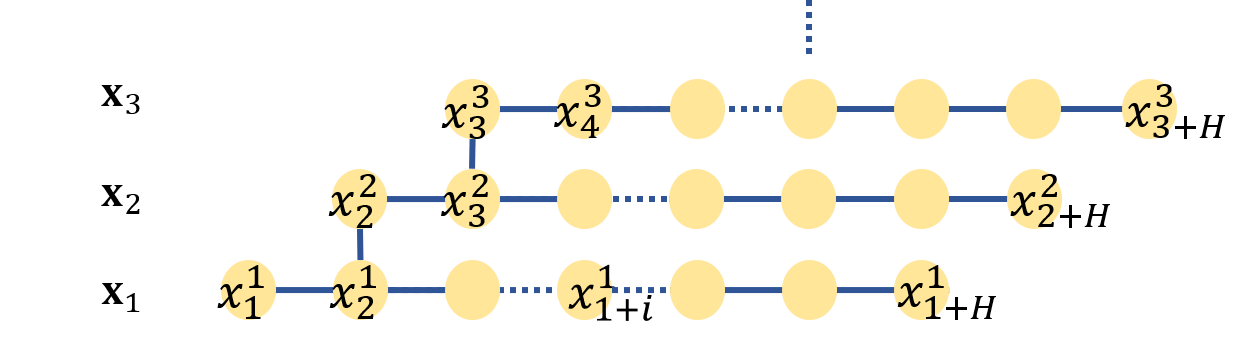
\includegraphics[width=8cm]{src/MPCstruc.png}
\caption{The execution structure of MPC}
\label{fig: mpc}
\end{center}
\end{figure}

\begin{figure}[t]
      \centering
      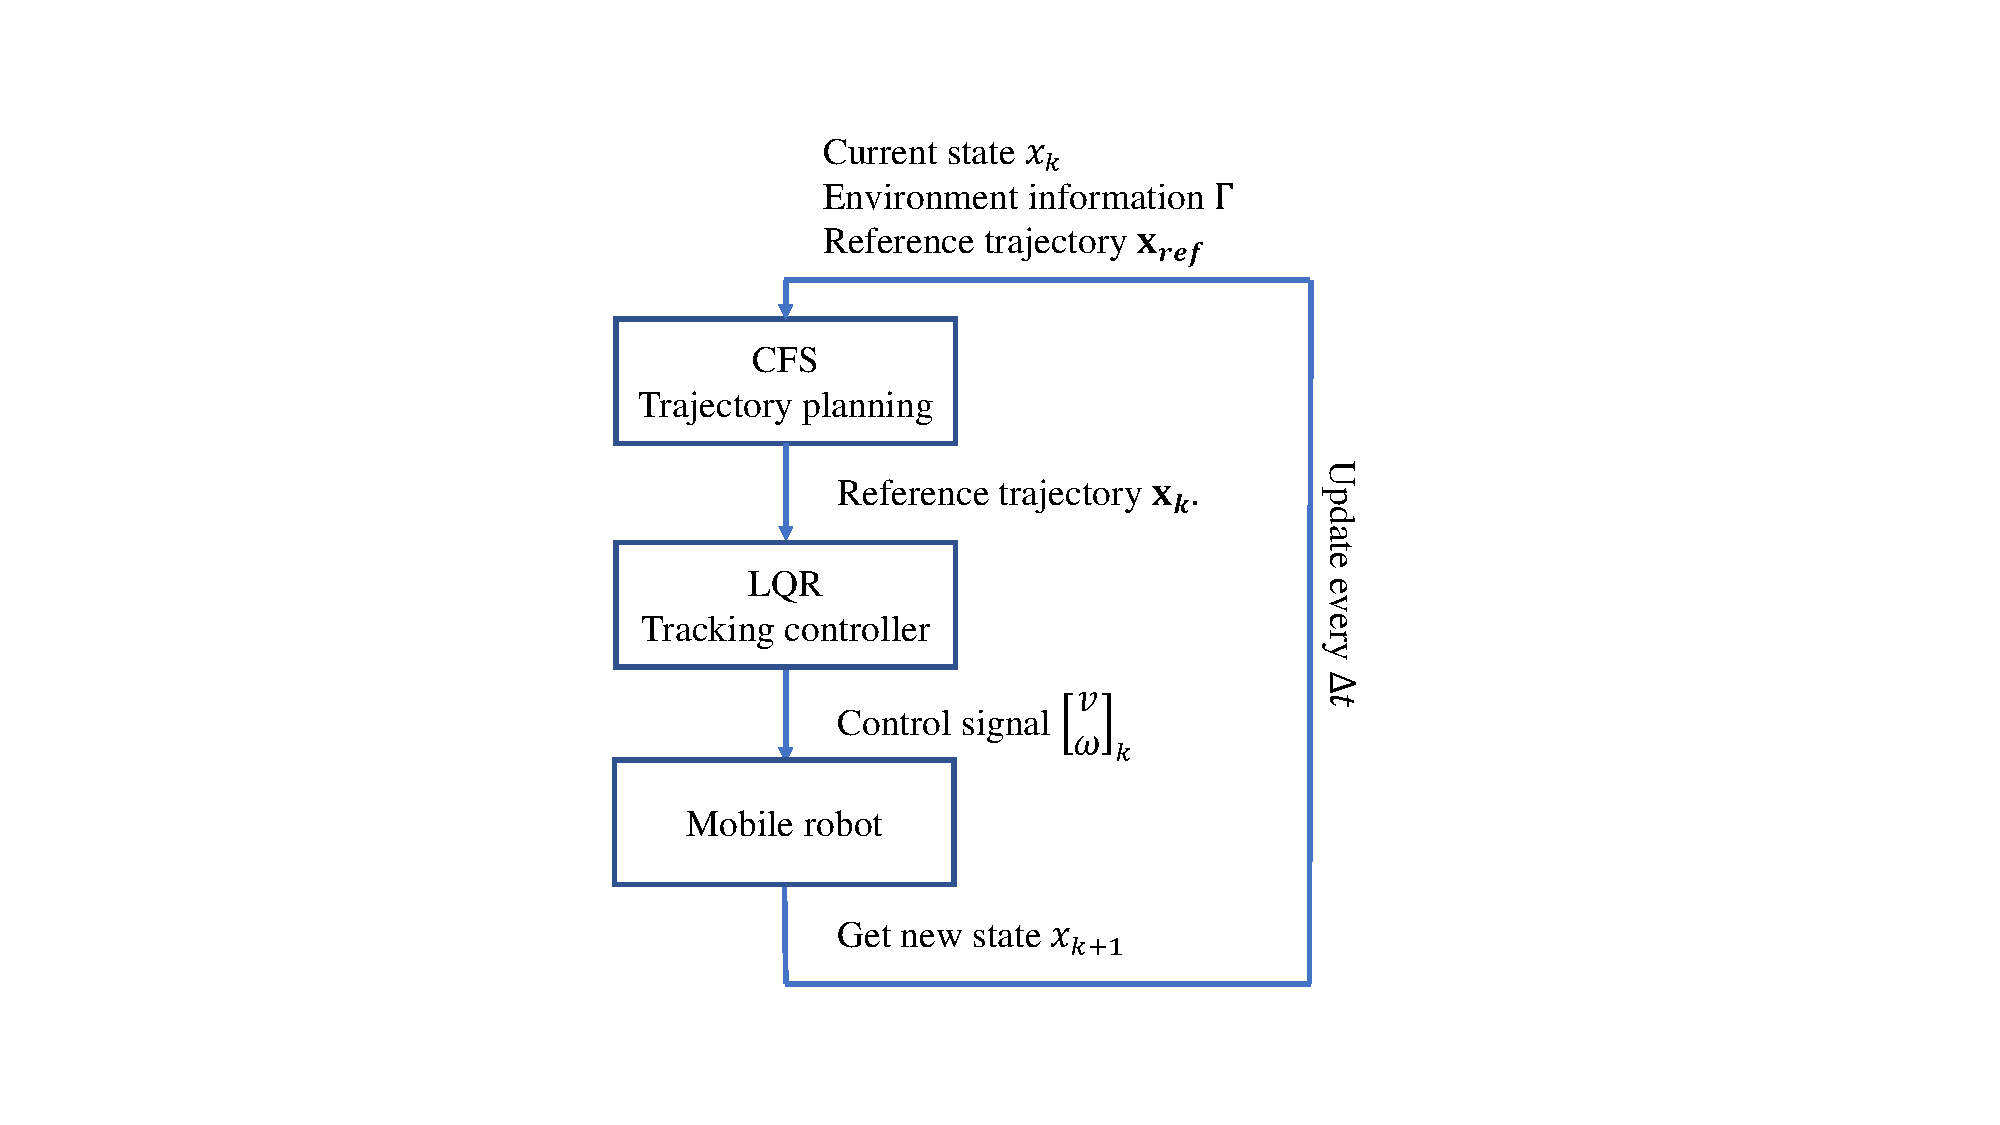
\includegraphics[width=6cm]{plot/MPCsystem.pdf}
      \caption{The overall system control design. }
      \label{fig:MPCsystem}
\end{figure}

\begin{figure}[t]
      \centering
      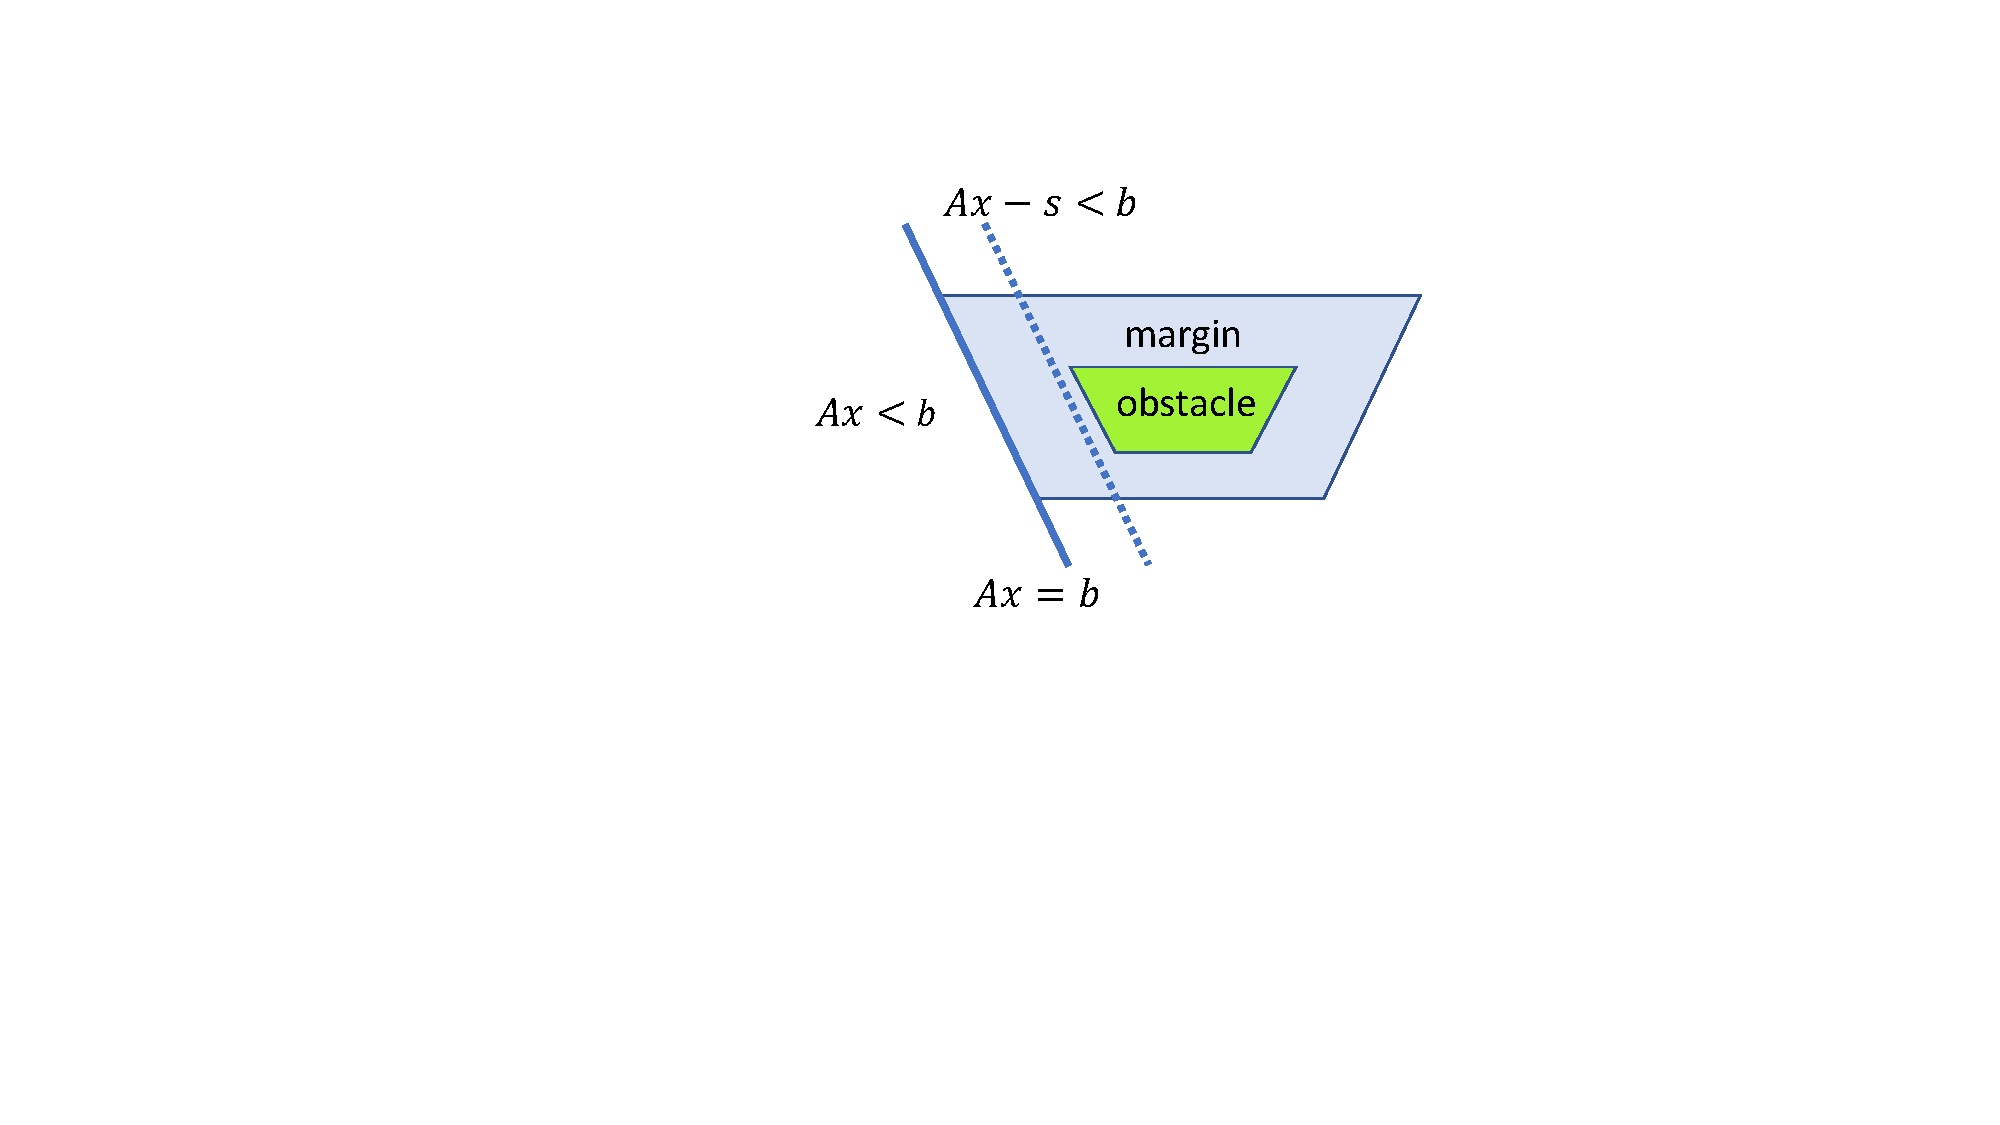
\includegraphics[width=5cm]{plot/slack.pdf}
      \caption{Illustration of the slack variable. }
      \label{fig:slack}
\end{figure}

\subsection{Problem and Notations}
In MPC (Fig.~\ref{fig:MPCsystem}), at each time step $t$, a future trajectory will be planned by solving an optimization problem. This trajectory is denoted as $\mathbf{x}_{k} := [x_k, x_{k+1},x_{k+2},\cdots,x_{k+H}]$ where the state, $x_k$, is called the $k^{th}$ action location. $H$ is the prediction horizon. In this paper, $x_k= [x(k)\quad y(k)]^{\intercal}$ that contains the $x$ and $y$ coordinate of the robot's location in 2-dimensional Cartesian space at time step $t=k$. Note that $x_k$ corresponds to the current position at time step $t=k$. The trajectory will then be executed and the robot will go to $x_{k+1}$, the $k+1^{th}$ action location, which is the planned action location for the robot at time step $t=k+1$. The sampling time between two time steps is a constant, denoted as $\Delta t$. After reaching the next action location, the robot will again solve the optimization problem and plan a new trajectory and repeat the process. To avoid confusion, the current time step can also be marked as superscript in some cases , e.g., $x_{k+1}^k$ means the planned action location $x_{k+1}$ at time step $t=k$.

At time step $k=t$, given the current state, denoted as $x_0(t=k) = (x,y)|_{t=k}$, the following optimization needs to be solved to obtain $\mathbf{x}_k$,


\begin{eqnarray}
&\min_{\mathbf{x}_{k}} & J(\mathbf{x}_k),\\
&s.t.& x_{k+i}\in\Gamma,\forall i=1,\ldots,H,\\
&&         x_{k}=x_0(k).
\end{eqnarray}

The current state is measured and assigned to the first entry of $\mathbf{x}_{k}$. Note that the optimization problem for each time step is time-invariant. There are two assumptions in this formulation: 

\begin{assumption}[Cost]
The cost function is convex and regular, and has the following form
\begin{equation}
J(\mathbf{x}_k) = C_1\|\mathbf{D}\mathbf{x}_k-\mathbf{d}\|_{2}^2 + C_2 \|\mathbf{V}\mathbf{x}_k-\mathbf{v}_{ref}\|_2^2 +C_3\|\mathbf{A}\mathbf{x}_{k}\|_2^2,  
\end{equation}
\end{assumption}
where $C_1$ is the coefficient of the first term, which penalizes the robot's deviation from a reference line so that the robot output trajectory is not too irregular. Matrix $\mathbf{D}$ is a projection matrix that extract all $y$'s from $\mathbf{x}_k$. $C_2$ is the coefficient of the second term, which penalizes the speed profile of the planned trajectory with regard to a constant speed so that the robot will be time efficient. $\mathbf{V}\mathbf{x}_k$ is the velocity vector. Here, the speed reference is set to be a constant speed going along the positive $x$-axis. $C_3$ is the coefficient of the third term, which penalizes the acceleration of the output trajectory so that the motion will be smooth. $\mathbf{A}\mathbf{x}_{k}$ is the acceleration vector.

\begin{assumption}[Constraint]
The state constraint $\Gamma$ is non-convex and its complement is a collection of disjoint convex sets, i.e., each of the obstacle-region is itself convex.
\end{assumption}

Since the robot dynamics is not included in the MPC problem, a tracking controller is needed. The overall system is shown in Fig.~\ref{fig:MPCsystem}. Although the planned trajectory  is feasible, tracking error will occur in real world experiment, causing the state ends up to be infeasible. This results in a violent motion because the control command according to the new planning result will immediately pull the robot out of the infeasible area. In order to avoid such problem, we introduce  $\mathbf{S}$, the slack variable vector. Introducing slack variables allows the states to violate the original constraint, which is the margin boundary of the obstacles (Fig.~\ref{fig:slack}). However these slack variables are also added to the cost function so that the violation is penalized \cite{chen2018foad}. The new problem is shown in the following:

\begin{eqnarray}
&\min_{\mathbf{x}_{k}} & J(\mathbf{x}_k) + \|\mathbf{S}\|_{2}^2 ,\\
&s.t.& x_{k+i} \in\Gamma(s_{k+i}),\forall i=1,\ldots,H,\\
&&         x_{k}=x_0(k).
\end{eqnarray} 

The final trajectory is $[x_k^k,x_{k+1}^{k+1},\ldots]$, which is equivalent to $[x_{k}^{k-1},x_{k+1}^{k},\ldots]$ (Fig.~\ref{fig: mpc}). As the problem is non-convex, it is possible that the planned trajectories calculated at different time steps enter into different local optima, hence the stability is hard to characterize. 

\subsection{$M$-Analysis for analyzing stability properties}
In this paper, we propose a new way, $M$-analysis, to analyzing stability properties.
We say that an action location, $x_{k}$, is $M$-settling if for $k-M< t\leq k$, the last $M$ time steps at $x_{k}$ satisfy: $\|x_{k}^t-x_k^{t-1}\|\leq \|x_k^{t-1}-x_k^{t-2}\|$ or $\bigl|\|x_{k}^t-x_k^{t-1}\|-\|x_k^{t-1}-x_k^{t-2}\|\bigr|\leq \delta$, where $\delta$ is a small threshold. In Fig.~\ref{fig:m-stable}, the pink-orange-color circles are the action location $x_{k}$ planned at different time steps that are  tested for $M$-settling property of $x_{k}$. The notation implies that the planned state $x_k$ would have smaller and smaller change on each predicted action location between consecutive time steps after time step $k-M$. Under the condition that the environment in the future time step is not going to change much, we say that the non-convex MPC is $M$-settling if the above inequalities holds for all $k$. This result can also be expressed as saying the output solutions are all close to one local optimum after time step $k-M$. Note that the problem is always $1$-settling, since $\|x_{k}^t-x_k^{t-1}\|=0$.

Having such property is good for the robot. $M$-analysis guarantees that the action location will not change much, and therefore, guarantees smoothness of the output trajectory. If M is sufficiently large, the robot system will not experience sudden change. Moreover, since the planned trajectory is usually tracked by a low-level tracking controller, the larger the $M$ is, the smoother the control commend would be.

\begin{figure}[t]
\begin{center}
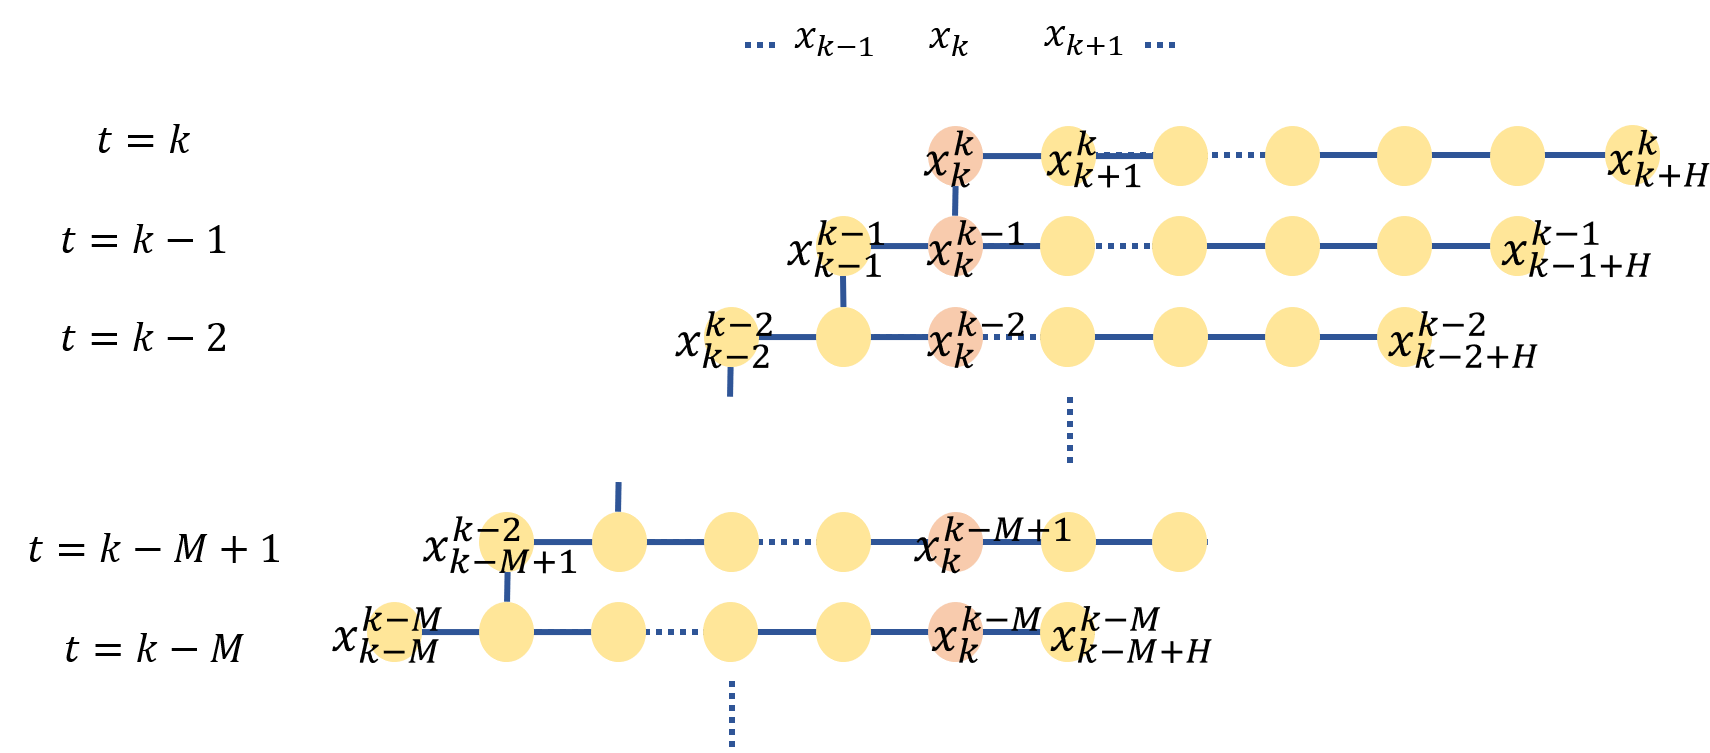
\includegraphics[width=9cm]{src/Mstable.png}
\caption{Illustration of $M$-analysis.}
\label{fig:m-stable}
\end{center}
\end{figure}


\subsection{The Convex Feasible Set Algorithm}
Because the problem we are solving has non-convex state constraints, the problem is a non-convex MPC problem. Here we solve the optimization problem at each MPC time step using the convex feasible set algorithm (CFS), which iteratively solve a sequence of sub-problems of the original non-convex problem using convex constraints, e.g., convex feasible set. The CFS algorithm in the MPC structure uses the previous solution, the planned action locations, as a reference. The convex feasible set for a reference point $x_r$ is computed as $\mathcal{F}(x_r) = \{x:A(x_r)x\leq b(x_r)\}$ where $A(x_r)$ is a matrix and $b(x_r)$ is a column vector. 
At time step $k+1$, the reference is set as $\mathbf{x}_{k+1}^{r}=[x_{k+1}^{k},x_{k+2}^{k},\ldots,x_{k+H}^k, x_{k+H+1}^*]$ where
\begin{equation}
\begin{split}
x_{k+H+1}^* & = \arg\min_{x_{k+H+1}} \|x_{k+H+1}\|_Q^2+\|x_{k+H}^k-x_{k+H+1}\|_R^2 \\
 & +\|x_{k+H-1}^k -2x_{k+H}^k+x_{k+H+1}\|_P^2\text{.}
\end{split}
\end{equation}
If $x_{k+H+1}^*\in\Gamma$, then the optimal solution is $\mathbf{x}_{k+1}^o = \mathbf{x}_{k+1}^r$.  If $x_{k+H+1}^*\notin\Gamma$, denote the feasible solution as 
\begin{equation}
\begin{split}
\bar{x}_{k+H+1} & = \arg\min_{x_{k+H+1}\in\Gamma} \|x_{k+H+1}\|_Q^2+\|x_{k+H}^k-x_{k+H+1}\|_R^2 \\
 & +\|x_{k+H-1}^k -2x_{k+H}^k+x_{k+H+1}\|_P^2 \text{.}
\end{split}
\end{equation}

Moreover, denote \\$\mathbf{x}_{k+1}^{u}:=[x_{k+1}^{k},x_{k+2}^{k},\ldots,x_{k+H}^k, \bar x_{k+H+1}]$. 

Because of the construction above, the optimal solution is $\mathbf{x}_{k+1}^{o}$ at step $k+1$ satisfies that
\begin{eqnarray}
\mathbf{x}_{k+1}^{o} = \arg\min_{x_{k+i}\in \mathcal{F}(x_{k+i}^o)}J(\mathbf{x}_{k+1}).
\end{eqnarray}
Note that $J(\mathbf{x}_{k+1}^{r})\leq J(\mathbf{x}_{k+1}^{o})\leq J(\mathbf{x}_{k+1}^{u})$, therefore, the cost of the trajectory is always bounded. 
The executed trajectory is from those $\mathbf{x}_{k+1}^{o}$ for different $k$.


\subsection{Converging property with CFS}
In this paper, we will show that the system is stable through simulation. Theoretical proof is left as future work. But here we sketch the procedures. First, we can show that at two consecutive time steps, the difference between the early state should be strictly smaller than the difference between any future state, i.e., $\|x_{k+i}^{k+1}-x_{k+i}^k\|<\lambda\|x_{k+i+1}^{k+1}-x_{k+i+1}^k\|$ for some $\lambda<1$ and for $i$ sufficiently small. Then we can show that the state is bounded and the difference between the same state at different time steps keeps decreasing.
%the KKT condition is satisfied, i.e.,
%\begin{eqnarray}
%2Qx_{k+i}^k +2R(2x_{k+i}^k-x_{k+i-1}^k-x_{k+i+1}^k) + \eta_{k+i}^k A(x_{k+i}^k) \nonumber\\
%= 0,\forall i=1,\ldots,H
%\end{eqnarray}
%where $\eta_{k+i}^k$ is the Lagrangian multiplier such that $\eta_{k+i}^k\geq 0$ and $\eta_{k+i}^k= 0$ if and only if $A(x_{k+i}^k)x_{k+i}^k= b(x_{k+i}^k)$.
%
%Hence
%\begin{eqnarray}
%(Q+2R)(x_{k+i}^{k+1}-x_{k+i}^k)=R(x_{k+i-1}^{k+1}-x_{k+i-1}^k)\\+R(x_{k+i+1}^{k+1}-x_{k+i+1}^k)-(\eta_{k+i}^{k+1} A(x_{k+i}^{k+1})-\eta_{k+i}^k A(x_{k+i}^k))
%\end{eqnarray}
%
%Claim that $\|x_{k+i}^{k+1}-x_{k+i}^k\|<\lambda\|x_{k+i+1}^{k+1}-x_{k+i+1}^k\|$ for some $\lambda<1$.


\section{SIMULATION RESULT AND DISCUSSION}
The simulation scenario in this work is similar to that of mobile robots operating in factories. To test our algorithm, three kinds of scenarios will be considered. The first one is a static scenario where the environment  is completely known, while the other two are dynamic scenarios where the robot will observe changes in the environment.
The goal for the robot is to move along a line, $y=0$, in the positive $x$-axis direction, while maintaining a constant speed which also points along the positive $x$-axis. 


\subsection{Result of scenario with single static obstacle}
In this scenario, there is only one static obstacle. This is the scenario as discussed in section 2, where the MPC problem is time invariant. 

The simulation result is shown in Fig.~\ref{fig:1_1}. In the figure, the planned trajectory is marked by gray-star-line of which the gray-color gets darker as time step increases. We can see that the robot successfully track the line while avoiding collision. It is clear from the figure that the last several action locations planned at each time step are one on top of another. This can be taken as an indication of stability. 


Figure~\ref{fig:single_m} shows the number $M$ for $M$-analysis at each action location. The result in Fig.~\ref{fig:single_m} shows that the system is 20-settling once it has run for a sufficient period of time. Note that 20-settling is the highest possible status that a system with prediction horizon of 20 can reach, which is the case in this simulation. If we decrease the sampling time to one fifth of the original, i.e, $\Delta t_{new}=0.2\Delta t_{original}$, it takes less time for the system to reach 20-settling (Fig.~\ref{fig:single_m}). In the figure, the system reaches 20-settling at the $49^{th}$ action location. The run-time at this point is almost equivalent to the run-time at the $10^{th}$ action location in Fig.~\ref{fig:single_m}. This result indicates that decreasing sampling time will increase $M$.

Notice that there is a high peak in $M$ around the $35^{th}$ action location in Fig.~\ref{fig:single_m_0.1Hz} (and a jump at $6^{th}$ in Fig.~\ref{fig:single_m}). This is because these action locations around the peak are close to the obstacle and do not have much space to be adjust. Therefore, these action locations do not change much throughout time and $M$ for $M$-analysis is higher. We call these action locations which are fixed due to the existence of the obstacle critical cation locations. After passing the critical action locations, the robot again has freedom to adjust its planning to best fit the cost function. The adjustment causes $M$ to drop, but soon after, the system reaches to 20-settling and perfectly track the line with constant speed. 

Another way to analyze stability is to look at the cost change. Define path$_k$ as $\mathbf{x}_{k}^{p} := [x_{k}^{k-1},x_{k+1}^{k},\ldots]$ (Fig.~\ref{fig:cost1}). Increase of the index $k$ means the path is starting further and further away from disturbance, i.e., the obstacle, which is located close to the robot's initial location. Therefore, it is expected that the cost will decrease as $k$ increases, which indicates that the robot is stably doing better and better according to what the cost function wants it to do. This expectation meets perfectly with Fig.~\ref{fig:costplot}. 


\begin{figure}[t]
      \centering
      \subfloat[ Simulation result of single static obstacle.\label{fig:1_1}]{% This file was created by matlab2tikz.
%
%The latest updates can be retrieved from
%  http://www.mathworks.com/matlabcentral/fileexchange/22022-matlab2tikz-matlab2tikz
%where you can also make suggestions and rate matlab2tikz.
%
\definecolor{mycolor1}{rgb}{0.96667,0.96667,0.96667}%
\definecolor{mycolor2}{rgb}{0.93333,0.93333,0.93333}%
\definecolor{mycolor3}{rgb}{0.86667,0.86667,0.86667}%
\definecolor{mycolor4}{rgb}{0.83333,0.83333,0.83333}%
%
\begin{tikzpicture}

\begin{axis}[%
width=7.5cm,
height=3cm,
at={(3in,1in)},
scale only axis,
xmin=-10,
xmax=70,
xlabel={$x$ [\si{\meter}]},
ymin=-3,
ymax=3,
font = \footnotesize,
ylabel style={at={(0.08, 0.5)}},
ylabel={$y$ [\si{\meter}]},
axis background/.style={fill=white},
legend style={legend cell align=left, align=left, draw=white!15!black}
]

\addplot[area legend, line width=1.0pt, draw=black, fill=green, forget plot]
table[row sep=crcr] {%
x	y\\
3	2.1\\
6.8	2.1\\
5.8	-1\\
3.8	-1\\
}--cycle;
\addplot [color=mycolor1, mark=asterisk, mark options={solid, mycolor1}, forget plot]
  table[row sep=crcr]{%
-6	0\\
-3.99540735382658	-0.142282650441845\\
-1.98629410632137	-0.404196422928299\\
0.0228547386424788	-0.720973472296906\\
2.03200385952139	-1.10006412633186\\
4.04115242415513	-1.50000000000074\\
6.05023006973479	-1.43350674327495\\
8.05030155169225	-1.09365162332893\\
10.0503021145776	-0.80326108430985\\
12.0503021190101	-0.585658663363307\\
14.0503021190451	-0.426477945853229\\
16.0503021190454	-0.310631702647056\\
18.0503021190454	-0.226466103205833\\
20.0503021190454	-0.165414684492027\\
22.0503021190454	-0.121248835502352\\
24.0503021190454	-0.0894604516082087\\
26.0503021190454	-0.0668043359074983\\
28.0503021190454	-0.0509664066612005\\
30.0503021190454	-0.0403213464486223\\
32.0503021190455	-0.0337249796870791\\
34.0503021190455	-0.0301159248247597\\
};


\addplot [color=blue, mark=o, mark options={solid, blue}, forget plot]
  table[row sep=crcr]{%
-3.99540735382658	-0.142282650441845\\
};
\addplot [color=mycolor2, mark=asterisk, mark options={solid, mycolor2}, forget plot]
  table[row sep=crcr]{%
-3.99540735382658	-0.142282650441845\\
-1.99067285034179	-0.32079027957026\\
0.0187218864350384	-0.660068999493075\\
2.02815331570448	-1.07181206954949\\
4.03758445824284	-1.50000000000015\\
6.04694249344227	-1.43493156830218\\
8.04701618332786	-1.09485799619372\\
10.0470167635992	-0.804107150400007\\
12.0470167681685	-0.586191531123407\\
14.0470167682045	-0.426746195951842\\
16.0470167682047	-0.310661857436718\\
18.0470167682047	-0.22626111343573\\
20.0470167682047	-0.164953605658893\\
22.0470167682047	-0.120484600219115\\
24.0470167682047	-0.0883150720851459\\
26.0470167682047	-0.0651610826452255\\
28.0470167682047	-0.0486588507152643\\
30.0470167682047	-0.0371228413383561\\
32.0470167682047	-0.0293692069652277\\
34.0470167682047	-0.0245645543963268\\
36.0470167682047	-0.0219357959706246\\
};
\addplot [color=blue, mark=o, mark options={solid, blue}, forget plot]
  table[row sep=crcr]{%
-1.99067285034179	-0.32079027957026\\
};
\addplot [color=white!90!black, mark=asterisk, mark options={solid, white!90!black}, forget plot]
  table[row sep=crcr]{%
-1.99067285034179	-0.32079027957026\\
0.0140061078955766	-0.561479022269409\\
2.02329062107169	-1.01787073351998\\
4.03261083179604	-1.50000000000008\\
6.04185907620916	-1.43765381777547\\
8.04193190154681	-1.09721986468783\\
10.0419324750102	-0.805851873755608\\
12.041932479526	-0.587423456431456\\
14.0419324795616	-0.427580155330739\\
16.0419324795619	-0.311181365970303\\
18.0419324795619	-0.226518964903045\\
20.0419324795619	-0.164976087162598\\
22.0419324795619	-0.120274001965129\\
24.0419324795619	-0.0878498976603945\\
26.0419324795619	-0.0643938660792609\\
28.0419324795619	-0.0475114138404029\\
30.0419324795619	-0.0354790112342423\\
32.0419324795619	-0.0270676697944878\\
34.0419324795619	-0.0214142012697563\\
36.0419324795619	-0.0179109470865368\\
38.0419324795619	-0.0159942197440002\\
};
\addplot [color=blue, mark=o, mark options={solid, blue}, forget plot]
  table[row sep=crcr]{%
0.0140061078955766	-0.561479022269409\\
};
\addplot [color=mycolor3, mark=asterisk, mark options={solid, mycolor3}, forget plot]
  table[row sep=crcr]{%
0.0140061078955766	-0.561479022269409\\
2.01824517500908	-0.916891024333778\\
4.02665629556289	-1.5\\
6.03503481384766	-1.44148226839047\\
8.0351007905234	-1.10056062990836\\
10.035101310057	-0.808348641030182\\
12.0351013141481	-0.589227791297892\\
14.0351013141803	-0.428860945467835\\
16.0351013141806	-0.312067092158574\\
18.0351013141806	-0.227099709858738\\
20.0351013141806	-0.165311086024793\\
22.0351013141806	-0.120397445513289\\
24.0351013141806	-0.0877743867805865\\
26.0351013141806	-0.0641116944204091\\
28.0351013141806	-0.0469937914988127\\
30.0351013141807	-0.0346732010645548\\
32.0351013141807	-0.0258921128536789\\
34.0351013141807	-0.0197536271868611\\
36.0351013141807	-0.0156278006782286\\
38.0351013141807	-0.0130711721394044\\
40.0351013141807	-0.0116723698919388\\
};
\addplot [color=blue, mark=o, mark options={solid, blue}, forget plot]
  table[row sep=crcr]{%
2.01824517500908	-0.916891024333778\\
};
\addplot [color=mycolor4, mark=asterisk, mark options={solid, mycolor4}, forget plot]
  table[row sep=crcr]{%
2.01824517500908	-0.916891024333778\\
4.02262790164366	-1.50000000000027\\
6.03125692555926	-1.44331521034021\\
8.03132487484263	-1.10215946862789\\
10.0313254099096	-0.809542631417147\\
12.031325414123	-0.590089343456519\\
14.0313254141561	-0.429470680036722\\
16.0313254141564	-0.312486167424506\\
18.0313254141564	-0.227370745906264\\
20.0313254141564	-0.165461727526063\\
22.0313254141564	-0.120443067065084\\
24.0313254141564	-0.0877196451376091\\
26.0313254141564	-0.0639510014929311\\
28.0313254141564	-0.0467107447255343\\
30.0313254141564	-0.0342389170698569\\
32.0313254141564	-0.0252623339561775\\
34.0313254141564	-0.0188645749898449\\
36.0313254141564	-0.0143921735348608\\
38.0313254141564	-0.0113861630170534\\
40.0313254141564	-0.00952344478070931\\
42.0313254141564	-0.00850430006891008\\
};
\addplot [color=blue, mark=o, mark options={solid, blue}, forget plot]
  table[row sep=crcr]{%
4.02262790164366	-1.50000000000027\\
};
\addplot [color=white!80!black, mark=asterisk, mark options={solid, white!80!black}, forget plot]
  table[row sep=crcr]{%
4.02262790164366	-1.50000000000027\\
6.02709217083431	-1.44620954739367\\
8.02712732473991	-1.10469060073017\\
10.0271276015595	-0.811442557147171\\
12.0271276037393	-0.591474028819655\\
14.0271276037565	-0.430469925626459\\
16.0271276037566	-0.313200268708197\\
18.0271276037566	-0.227872347766933\\
20.0271276037566	-0.165801998035618\\
22.0271276037566	-0.120656736913482\\
24.0271276037566	-0.087828525827847\\
26.0271276037566	-0.0639662079317938\\
28.0271276037566	-0.0466338294123891\\
30.0271276037566	-0.0340620293740457\\
32.0271276037566	-0.024967424620289\\
34.0271276037566	-0.0184215936905541\\
36.0271276037566	-0.0137562719342408\\
38.0271276037566	-0.01049494372258\\
40.0271276037566	-0.00830292518294445\\
42.0271276037566	-0.00694460894154336\\
44.0271276037566	-0.00620143652428602\\
};


\addplot [color=blue, mark=o, mark options={solid, blue}, forget plot]
  table[row sep=crcr]{%
6.02709217083431	-1.44620954739367\\
};
\addplot [color=black!8!mycolor4, mark=asterisk, mark options={solid, black!8!mycolor4}, forget plot]
  table[row sep=crcr]{%
6.02709217083431	-1.44620954739367\\
8.02709217083437	-1.21162151084362\\
10.0270921708344	-0.905073249081907\\
12.0270921708345	-0.661932838169451\\
14.0270921708346	-0.482070983872636\\
16.0270921708346	-0.350784755951799\\
18.0270921708346	-0.255213864111262\\
20.0270921708346	-0.18568232048145\\
22.0270921708346	-0.135103946191281\\
24.0270921708346	-0.0983172488276095\\
26.0270921708345	-0.0715671475144989\\
28.0270921708345	-0.0521229172152845\\
30.0270921708344	-0.037999614205722\\
32.0270921708343	-0.027755472602289\\
34.0270921708343	-0.0203447264492765\\
36.0270921708342	-0.0150108507418865\\
38.0270921708341	-0.0112093094786808\\
40.0270921708341	-0.00855181350802617\\
42.0270921708341	-0.00676564540148995\\
44.0270921708341	-0.0056588202970963\\
46.0270921708341	-0.00505324564279711\\
};
\addplot [color=blue, mark=o, mark options={solid, blue}, forget plot]
  table[row sep=crcr]{%
8.02709217083437	-1.21162151084362\\
};
\addplot [color=black!12!mycolor4, mark=asterisk, mark options={solid, black!12!mycolor4}, forget plot]
  table[row sep=crcr]{%
8.02709217083437	-1.21162151084362\\
10.0270921708338	-1.01508573787531\\
12.0270921708325	-0.758262327511277\\
14.0270921708313	-0.554561451280546\\
16.0270921708301	-0.403874787622836\\
18.0270921708289	-0.293884352202541\\
20.0270921708277	-0.213815908059347\\
22.0270921708265	-0.155562998516528\\
24.0270921708254	-0.113188885868714\\
26.0270921708244	-0.0823693176262817\\
28.0270921708235	-0.0599583203910789\\
30.0270921708226	-0.0436681169868297\\
32.0270921708218	-0.0318357391953659\\
34.0270921708212	-0.023253288367945\\
36.0270921708206	-0.0170446310773274\\
38.0270921708201	-0.0125759573953628\\
40.0270921708197	-0.00939105989762989\\
42.0270921708194	-0.00716463338239732\\
44.0270921708192	-0.00566819761092024\\
46.0270921708191	-0.00474090937141255\\
48.027092170819	-0.00423356430592784\\
};


\addplot [color=blue, mark=o, mark options={solid, blue}, forget plot]
  table[row sep=crcr]{%
10.0270921708338	-1.01508573787531\\
};
\addplot [color=white!70!black, mark=asterisk, mark options={solid, white!70!black}, forget plot]
  table[row sep=crcr]{%
10.0270921708338	-1.01508573787531\\
12.0270921708332	-0.85042981328417\\
14.027092170832	-0.63526544167151\\
16.0270921708309	-0.464606657221156\\
18.0270921708297	-0.338362709092185\\
20.0270921708286	-0.246213699439784\\
22.0270921708274	-0.179133068255699\\
24.0270921708264	-0.130329298153021\\
26.0270921708253	-0.094828643023511\\
28.0270921708243	-0.0690082825475464\\
30.0270921708234	-0.050232548160637\\
32.0270921708226	-0.0365847604688608\\
34.0270921708218	-0.0266716994726631\\
36.0270921708212	-0.0194813984149648\\
38.0270921708206	-0.0142798404938954\\
40.0270921708202	-0.0105360253823455\\
42.0270921708198	-0.00786774655302809\\
44.0270921708195	-0.0060024661979049\\
46.0270921708194	-0.00474876560274523\\
48.0270921708192	-0.00397189175362465\\
50.0270921708192	-0.00354684256496818\\
};
\addplot [color=blue, mark=o, mark options={solid, blue}, forget plot]
  table[row sep=crcr]{%
12.0270921708332	-0.85042981328417\\
};
\addplot [color=black!20!mycolor4, mark=asterisk, mark options={solid, black!20!mycolor4}, forget plot]
  table[row sep=crcr]{%
12.0270921708332	-0.85042981328417\\
14.0270921708325	-0.712482542446397\\
16.0270921708314	-0.532219743405386\\
18.0270921708302	-0.389243329906362\\
20.0270921708291	-0.283477271700997\\
22.0270921708279	-0.206275650055698\\
24.0270921708268	-0.150076093186482\\
26.0270921708257	-0.109188728161674\\
28.0270921708246	-0.0794465946779907\\
30.0270921708236	-0.0578145260563892\\
32.0270921708227	-0.0420843825885281\\
34.0270921708218	-0.0306503873057492\\
36.0270921708211	-0.0223453128696389\\
38.0270921708204	-0.0163213425213174\\
40.0270921708199	-0.0119635235051009\\
42.0270921708194	-0.00882698846428367\\
44.0270921708191	-0.006591528165783\\
46.0270921708188	-0.00502881285521743\\
48.0270921708187	-0.00397847363434414\\
50.0270921708186	-0.003327615625225\\
52.0270921708185	-0.00297151319106767\\
};


\addplot [color=blue, mark=o, mark options={solid, blue}, forget plot]
  table[row sep=crcr]{%
14.0270921708325	-0.712482542446397\\
};
\addplot [color=black!24!mycolor4, mark=asterisk, mark options={solid, black!24!mycolor4}, forget plot]
  table[row sep=crcr]{%
14.0270921708325	-0.712482542446397\\
16.0270921708319	-0.596911544446537\\
18.0270921708307	-0.445888972844418\\
20.0270921708295	-0.326104603801337\\
22.0270921708283	-0.237494739850683\\
24.0270921708272	-0.17281590708681\\
26.0270921708261	-0.12573241761235\\
28.0270921708249	-0.0914773464333292\\
30.0270921708239	-0.0665596512264677\\
32.0270921708228	-0.0484364963121448\\
34.0270921708219	-0.0352579218595819\\
36.027092170821	-0.0256786221899833\\
38.0270921708202	-0.0187207046087462\\
40.0270921708196	-0.013673875767192\\
42.027092170819	-0.010022933709781\\
44.0270921708186	-0.00739517251721642\\
46.0270921708182	-0.00552232373872311\\
48.027092170818	-0.00421309473453418\\
50.0270921708178	-0.00333312986639852\\
52.0270921708177	-0.00278784680852218\\
54.0270921708177	-0.00248950735276915\\
};
\addplot [color=blue, mark=o, mark options={solid, blue}, forget plot]
  table[row sep=crcr]{%
16.0270921708319	-0.596911544446537\\
};
\addplot [color=white!60!black, mark=asterisk, mark options={solid, white!60!black}, forget plot]
  table[row sep=crcr]{%
16.0270921708319	-0.596911544446537\\
18.0270921708312	-0.500087189042005\\
20.02709217083	-0.373561820221298\\
22.0270921708287	-0.273207539987887\\
24.0270921708275	-0.198970983170123\\
26.0270921708263	-0.144783631680056\\
28.0270921708251	-0.1053375024828\\
30.0270921708239	-0.0766389081672282\\
32.0270921708228	-0.055763084488923\\
34.0270921708218	-0.0405796663057666\\
36.0270921708208	-0.0295387737063714\\
38.0270921708198	-0.0215133215445907\\
40.027092170819	-0.0156840400083781\\
42.0270921708183	-0.0114558516403793\\
44.0270921708177	-0.00839712481924047\\
46.0270921708172	-0.0061956098368522\\
48.0270921708169	-0.00462655376842085\\
50.0270921708166	-0.00352969333977021\\
52.0270921708164	-0.00279246659077144\\
54.0270921708163	-0.00233563328913033\\
56.0270921708163	-0.00208568714352468\\
};
\addplot [color=blue, mark=o, mark options={solid, blue}, forget plot]
  table[row sep=crcr]{%
18.0270921708312	-0.500087189042005\\
};
\addplot [color=black!32!mycolor4, mark=asterisk, mark options={solid, black!32!mycolor4}, forget plot]
  table[row sep=crcr]{%
18.0270921708312	-0.500087189042005\\
20.0270921708305	-0.418968604260778\\
22.0270921708292	-0.312966774299948\\
24.0270921708279	-0.228890849856554\\
26.0270921708266	-0.166696122063879\\
28.0270921708254	-0.121298440379863\\
30.0270921708242	-0.0882508237733982\\
32.027092170823	-0.0642073964109087\\
34.0270921708218	-0.0467178167916972\\
36.0270921708207	-0.0339972839256235\\
38.0270921708197	-0.024747322191889\\
40.0270921708187	-0.0180236696679531\\
42.0270921708179	-0.0131399493835873\\
44.0270921708171	-0.00959761073162367\\
46.0270921708165	-0.00703503657426002\\
48.027092170816	-0.0051906268800338\\
50.0270921708156	-0.00387608564523176\\
52.0270921708154	-0.00295714572250831\\
54.0270921708152	-0.00233950370165293\\
56.0270921708151	-0.00195677282000802\\
58.027092170815	-0.0017473701597232\\
};
\addplot [color=blue, mark=o, mark options={solid, blue}, forget plot]
  table[row sep=crcr]{%
20.0270921708305	-0.418968604260778\\
};
\addplot [color=black!36!mycolor4, mark=asterisk, mark options={solid, black!36!mycolor4}, forget plot]
  table[row sep=crcr]{%
20.0270921708305	-0.418968604260778\\
22.0270921708298	-0.351008174579456\\
24.0270921708284	-0.262200783146619\\
26.0270921708271	-0.191762720569019\\
28.0270921708258	-0.139656530155305\\
30.0270921708246	-0.101622755748359\\
32.0270921708234	-0.0739357561467917\\
34.0270921708222	-0.0537923863016144\\
36.027092170821	-0.0391397718721008\\
38.0270921708199	-0.0284826224446839\\
40.0270921708189	-0.0207330866797727\\
42.0270921708179	-0.0151000703273825\\
44.0270921708171	-0.0110085328595546\\
46.0270921708164	-0.00804079300667354\\
48.0270921708157	-0.00589389114325601\\
50.0270921708153	-0.00434866108696828\\
52.0270921708149	-0.00324735011869925\\
54.0270921708146	-0.00247747041521544\\
56.0270921708145	-0.00196001541722106\\
58.0270921708144	-0.00163936688473132\\
60.0270921708144	-0.00146393119626454\\
};
\addplot [color=blue, mark=o, mark options={solid, blue}, forget plot]
  table[row sep=crcr]{%
22.0270921708298	-0.351008174579456\\
};
\addplot [color=gray, mark=asterisk, mark options={solid, gray}, forget plot]
  table[row sep=crcr]{%
22.0270921708298	-0.351008174579456\\
24.0270921708291	-0.294071530345262\\
26.0270921708276	-0.219669486757717\\
28.0270921708262	-0.160657103694045\\
30.0270921708248	-0.117003000270992\\
32.0270921708235	-0.0851386419606483\\
34.0270921708223	-0.0619427196626638\\
36.027092170821	-0.0450667833578179\\
38.0270921708198	-0.0327909531609537\\
40.0270921708186	-0.0238624880475777\\
42.0270921708175	-0.0173699958297319\\
44.0270921708165	-0.0126507047727741\\
46.0270921708156	-0.00922285103097878\\
48.0270921708149	-0.00673650494729788\\
50.0270921708142	-0.00493784963896211\\
52.0270921708137	-0.00364326962546044\\
54.0270921708133	-0.00272060108017848\\
56.027092170813	-0.00207560270413894\\
58.0270921708128	-0.00164208350384693\\
60.0270921708127	-0.0013734470119466\\
62.0270921708127	-0.00122646855071015\\
};
\addplot [color=blue, mark=o, mark options={solid, blue}, forget plot]
  table[row sep=crcr]{%
24.0270921708291	-0.294071530345262\\
};
\addplot [color=black!50!mycolor2, mark=asterisk, mark options={solid, black!50!mycolor2}, forget plot]
  table[row sep=crcr]{%
24.0270921708291	-0.294071530345262\\
26.0270921708283	-0.246370515624603\\
28.0270921708268	-0.184037144486355\\
30.0270921708253	-0.134597094215\\
32.0270921708239	-0.0980240741853319\\
34.0270921708226	-0.0713283978723223\\
36.0270921708213	-0.0518950602410534\\
38.02709217082	-0.0377565507287851\\
40.0270921708187	-0.0274719692469512\\
42.0270921708176	-0.0199917804944425\\
44.0270921708164	-0.0145524281928951\\
46.0270921708154	-0.0105986480710182\\
48.0270921708145	-0.00772682265880167\\
50.0270921708137	-0.00564378399830841\\
52.027092170813	-0.00413688656003654\\
54.0270921708125	-0.00305229892563378\\
56.0270921708121	-0.00227929541529072\\
58.0270921708118	-0.00173892150595193\\
60.0270921708117	-0.00137572297129854\\
62.0270921708116	-0.00115066170493481\\
64.0270921708115	-0.00102752445586111\\
};
\addplot [color=blue, mark=o, mark options={solid, blue}, forget plot]
  table[row sep=crcr]{%
26.0270921708283	-0.246370515624603\\
};
\addplot [color=black!50!mycolor3, mark=asterisk, mark options={solid, black!50!mycolor3}, forget plot]
  table[row sep=crcr]{%
26.0270921708283	-0.246370515624603\\
28.0270921708275	-0.206407029262091\\
30.0270921708259	-0.154184684685135\\
32.0270921708244	-0.112764249787656\\
34.027092170823	-0.0821236985174162\\
36.0270921708217	-0.0597582980637833\\
38.0270921708203	-0.0434772204399095\\
40.0270921708191	-0.0316321027754709\\
42.0270921708178	-0.0230157717770603\\
44.0270921708166	-0.0167489360933623\\
46.0270921708155	-0.0121918950577137\\
48.0270921708145	-0.00887945319653496\\
50.0270921708135	-0.00647346337914635\\
52.0270921708127	-0.00472831209486173\\
54.0270921708121	-0.00346584680818493\\
56.0270921708115	-0.00255718892344208\\
58.0270921708112	-0.00190957344976303\\
60.0270921708109	-0.00145685298915374\\
62.0270921708107	-0.00115256848345126\\
64.0270921708107	-0.000964014153924572\\
66.0270921708106	-0.000860850860598165\\
};
\addplot [color=blue, mark=o, mark options={solid, blue}, forget plot]
  table[row sep=crcr]{%
28.0270921708275	-0.206407029262091\\
};
\addplot [color=white!40!black, mark=asterisk, mark options={solid, white!40!black}, forget plot]
  table[row sep=crcr]{%
28.0270921708275	-0.206407029262091\\
30.0270921708266	-0.172925975418701\\
32.027092170825	-0.129174559069575\\
34.0270921708235	-0.0944728866869671\\
36.027092170822	-0.068802505039991\\
38.0270921708206	-0.0500649712316597\\
40.0270921708193	-0.036424829037658\\
42.0270921708179	-0.0265010946890961\\
44.0270921708167	-0.0192824091251481\\
46.0270921708154	-0.014032109863208\\
48.0270921708143	-0.0102142613677757\\
50.0270921708132	-0.00743912700383315\\
52.0270921708122	-0.00542341010936038\\
54.0270921708114	-0.00396133786710969\\
56.0270921708107	-0.00290365566553109\\
58.0270921708102	-0.00214239016211271\\
60.0270921708098	-0.00159982367161706\\
62.0270921708095	-0.00122053849164957\\
64.0270921708093	-0.000965611636016265\\
66.0270921708092	-0.000807642493847992\\
68.0270921708092	-0.000721213203200248\\
};
\addplot [color=blue, mark=o, mark options={solid, blue}, forget plot]
  table[row sep=crcr]{%
30.0270921708266	-0.172925975418701\\
};
\addplot [color=black!56!mycolor4, mark=asterisk, mark options={solid, black!56!mycolor4}, forget plot]
  table[row sep=crcr]{%
30.0270921708266	-0.172925975418701\\
32.0270921708257	-0.144875845950633\\
34.0270921708241	-0.108221298016008\\
36.0270921708226	-0.0791485451796295\\
38.0270921708211	-0.0576421274885957\\
40.0270921708197	-0.0419439881261388\\
42.0270921708183	-0.0305163981735105\\
44.027092170817	-0.022202381697637\\
46.0270921708157	-0.0161546310621572\\
48.0270921708145	-0.0117559769835709\\
50.0270921708134	-0.00855741743142888\\
52.0270921708123	-0.00623243451529153\\
54.0270921708113	-0.00454368480849687\\
56.0270921708105	-0.00331877367281957\\
58.0270921708098	-0.00243265692066594\\
60.0270921708093	-0.00179487544490337\\
62.0270921708088	-0.00134031805927492\\
64.0270921708086	-0.00102255630503794\\
66.0270921708084	-0.000808980850144505\\
68.0270921708083	-0.0006766357062296\\
70.0270921708083	-0.000604226014362994\\
};
\addplot [color=blue, mark=o, mark options={solid, blue}, forget plot]
  table[row sep=crcr]{%
32.0270921708257	-0.144875845950633\\
};
\addplot [color=black!60!mycolor4, mark=asterisk, mark options={solid, black!60!mycolor4}, forget plot]
  table[row sep=crcr]{%
32.0270921708257	-0.144875845950633\\
34.0270921708249	-0.121375696676483\\
36.0270921708232	-0.0906668420517427\\
38.0270921708216	-0.0663099480045037\\
40.0270921708201	-0.0482920623235687\\
42.0270921708187	-0.0351403006262253\\
44.0270921708173	-0.0255663672853535\\
46.027092170816	-0.0186009581426655\\
48.0270921708147	-0.0135342063878023\\
50.0270921708134	-0.00984905307791012\\
52.0270921708123	-0.00716932830076357\\
54.0270921708112	-0.00522147826850279\\
56.0270921708102	-0.00380665876680509\\
58.0270921708094	-0.00278043909930218\\
60.0270921708087	-0.00203805835650823\\
62.0270921708081	-0.00150373070209698\\
64.0270921708077	-0.00112290656266276\\
66.0270921708074	-0.00085668858793513\\
68.0270921708073	-0.000677756969219988\\
70.0270921708072	-0.000566879383400804\\
72.0270921708072	-0.00050621518684438\\
};
\addlegendentry{Path planned at each time step}


\addplot [color=blue, mark=o, mark options={solid, blue}, forget plot]
  table[row sep=crcr]{%
34.0270921708249	-0.121375696676483\\
};
\addplot [color=white!30!black, mark=asterisk, mark options={solid, white!30!black}, forget plot]
  table[row sep=crcr]{%
34.0270921708249	-0.121375696676483\\
36.0270921708239	-0.101687480387287\\
38.0270921708221	-0.0759598747966967\\
40.0270921708205	-0.0555538853478396\\
42.0270921708189	-0.0404586607932391\\
44.0270921708174	-0.029440231681995\\
46.027092170816	-0.0214192753827761\\
48.0270921708146	-0.0155837174829552\\
50.0270921708133	-0.0113388378751892\\
52.027092170812	-0.00825144917064878\\
54.0270921708108	-0.006006399558724\\
56.0270921708097	-0.00437450810616906\\
58.0270921708086	-0.00318918489673648\\
60.0270921708077	-0.0023294271761172\\
62.027092170807	-0.00170746718502989\\
64.0270921708064	-0.00125981222307422\\
66.027092170806	-0.000940761142263203\\
68.0270921708057	-0.000717726088098975\\
70.0270921708055	-0.000567818767561777\\
72.0270921708054	-0.000474926511199651\\
74.0270921708054	-0.00042410258626837\\
};
\addplot [color=blue, mark=o, mark options={solid, blue}, forget plot]
  table[row sep=crcr]{%
36.0270921708239	-0.101687480387287\\
};
\addplot [color=black!68!mycolor4, mark=asterisk, mark options={solid, black!68!mycolor4}, forget plot]
  table[row sep=crcr]{%
36.0270921708239	-0.101687480387287\\
38.027092170823	-0.0851928676881003\\
40.0270921708212	-0.0636385082854652\\
42.0270921708195	-0.0465425516097403\\
44.0270921708179	-0.03389590658219\\
46.0270921708164	-0.024664764559293\\
48.0270921708149	-0.0179448786290976\\
50.0270921708135	-0.0130559000630796\\
52.0270921708122	-0.00949957763873228\\
54.0270921708109	-0.0069129908100824\\
56.0270921708097	-0.00503210818997544\\
58.0270921708085	-0.00366492402855773\\
60.0270921708075	-0.00267187077396558\\
62.0270921708066	-0.00195157339361599\\
64.0270921708058	-0.00143050083850375\\
66.0270921708052	-0.00105545948829647\\
68.0270921708048	-0.000788161327214622\\
70.0270921708045	-0.000601304540265803\\
72.0270921708044	-0.000475713518893191\\
74.0270921708043	-0.00039788921177037\\
76.0270921708043	-0.00035530937898669\\
};
\addplot [color=blue, mark=o, mark options={solid, blue}, forget plot]
  table[row sep=crcr]{%
38.027092170823	-0.0851928676881003\\
};
\addplot [color=black!75!mycolor2, mark=asterisk, mark options={solid, black!75!mycolor2}, forget plot]
  table[row sep=crcr]{%
38.027092170823	-0.0851928676881003\\
40.027092170822	-0.0713738277050089\\
42.0270921708201	-0.0533157768839928\\
44.0270921708184	-0.0389929362596389\\
46.0270921708167	-0.028397689406946\\
48.0270921708152	-0.0206639206286088\\
50.0270921708137	-0.0150340598950184\\
52.0270921708123	-0.0109381170855565\\
54.0270921708109	-0.00795866175241302\\
56.0270921708096	-0.00579164228631703\\
58.0270921708083	-0.00421585553673672\\
60.0270921708072	-0.00307044079220412\\
62.0270921708061	-0.00223846959767259\\
64.0270921708052	-0.00163501085145076\\
66.0270921708044	-0.00119846089392544\\
68.0270921708038	-0.000884254582549373\\
70.0270921708033	-0.000660314557849044\\
72.027092170803	-0.000503767601769236\\
74.0270921708029	-0.000398548559813143\\
76.0270921708028	-0.000333348046700858\\
78.0270921708028	-0.000297675041078764\\
};
\addplot [color=blue, mark=o, mark options={solid, blue}, forget plot]
  table[row sep=crcr]{%
40.027092170822	-0.0713738277050089\\
};
\addplot [color=white!20!black, mark=asterisk, mark options={solid, white!20!black}, forget plot]
  table[row sep=crcr]{%
40.027092170822	-0.0713738277050089\\
42.027092170821	-0.0597963587739749\\
44.0270921708191	-0.044667484221827\\
46.0270921708173	-0.0326679355892605\\
48.0270921708156	-0.0237913319030724\\
50.0270921708141	-0.0173120491265317\\
52.0270921708126	-0.012595401818996\\
54.0270921708111	-0.00916385732113632\\
56.0270921708097	-0.00666769611218143\\
58.0270921708084	-0.00485218645504414\\
60.0270921708071	-0.0035320063153539\\
62.0270921708059	-0.0025723880181132\\
64.0270921708048	-0.00187536994246552\\
66.0270921708038	-0.00136979756593443\\
68.027092170803	-0.00100405988977783\\
70.0270921708024	-0.000740820633482476\\
72.0270921708019	-0.000553205670253332\\
74.0270921708016	-0.000422052021206049\\
76.0270921708014	-0.000333900442622432\\
78.0270921708013	-0.000279276031983614\\
80.0270921708013	-0.000249389504797928\\
};
\addplot [color=blue, mark=o, mark options={solid, blue}, forget plot]
  table[row sep=crcr]{%
42.027092170821	-0.0597963587739749\\
};
\addplot [color=black!80!mycolor4, mark=asterisk, mark options={solid, black!80!mycolor4}, forget plot]
  table[row sep=crcr]{%
42.027092170821	-0.0597963587739749\\
44.0270921708199	-0.0500968581564896\\
46.027092170818	-0.0374220214599267\\
48.0270921708162	-0.0273689062182149\\
50.0270921708145	-0.0199321665086917\\
52.0270921708129	-0.0145038809597436\\
54.0270921708114	-0.0105523157476711\\
56.0270921708099	-0.00767739825283223\\
58.0270921708085	-0.00558613656759215\\
60.0270921708071	-0.00406511870562714\\
62.0270921708059	-0.00295908351292266\\
64.0270921708047	-0.00215512382862849\\
66.0270921708036	-0.00157116827707332\\
68.0270921708026	-0.00114760423145742\\
70.0270921708018	-0.000841192455542852\\
72.0270921708012	-0.000620652945208114\\
74.0270921708007	-0.000463470795771326\\
76.0270921708004	-0.000353591433764208\\
78.0270921708002	-0.000279738824368314\\
80.0270921708001	-0.000233974978424665\\
82.0270921708001	-0.000208936311466477\\
};
\addplot [color=blue, mark=o, mark options={solid, blue}, forget plot]
  table[row sep=crcr]{%
44.0270921708199	-0.0500968581564896\\
};
\addplot [color=black!84!mycolor4, mark=asterisk, mark options={solid, black!84!mycolor4}, forget plot]
  table[row sep=crcr]{%
44.0270921708199	-0.0500968581564896\\
46.0270921708189	-0.041970702708436\\
48.0270921708169	-0.0313518371258859\\
50.0270921708151	-0.0229294264871367\\
52.0270921708134	-0.0166989920256736\\
54.0270921708117	-0.0121512226170614\\
56.0270921708102	-0.0088406363876647\\
58.0270921708087	-0.00643205605094513\\
60.0270921708073	-0.00468001558959174\\
62.027092170806	-0.00340572033739036\\
64.0270921708047	-0.00247909387883114\\
66.0270921708034	-0.00180554359761007\\
68.0270921708023	-0.0013163108243048\\
70.0270921708014	-0.000961452629776662\\
72.0270921708006	-0.000704743566039908\\
74.0270921707999	-0.000519977523530817\\
76.0270921707994	-0.000388291715127134\\
78.0270921707991	-0.000296235761803494\\
80.0270921707989	-0.000234362701762329\\
82.0270921707988	-0.000196022158203826\\
84.0270921707988	-0.000175044985476288\\
};
\addplot [color=blue, mark=o, mark options={solid, blue}, forget plot]
  table[row sep=crcr]{%
46.0270921708189	-0.041970702708436\\
};
\addplot [color=white!10!black, mark=asterisk, mark options={solid, white!10!black}, forget plot]
  table[row sep=crcr]{%
46.0270921708189	-0.041970702708436\\
48.0270921708178	-0.0351626818659107\\
50.0270921708158	-0.0262662906176643\\
52.0270921708139	-0.0192100698082807\\
54.0270921708121	-0.0139902671669621\\
56.0270921708105	-0.0101801863583169\\
58.0270921708089	-0.00740660662622093\\
60.0270921708074	-0.00538871941768702\\
62.0270921708059	-0.00392087548410295\\
64.0270921708045	-0.00285328224250588\\
66.0270921708032	-0.00207696282756675\\
68.0270921708019	-0.00151266838569794\\
70.0270921708008	-0.00110279351450388\\
72.0270921707998	-0.000805496471641812\\
74.0270921707989	-0.000590427898614001\\
76.0270921707982	-0.000435632549641366\\
78.0270921707977	-0.000325307349248162\\
80.0270921707974	-0.000248183689377988\\
82.0270921707972	-0.000196346989360929\\
84.0270921707971	-0.000164225622592712\\
86.0270921707971	-0.000146651133649645\\
};
\addplot [color=blue, mark=o, mark options={solid, blue}, forget plot]
  table[row sep=crcr]{%
48.0270921708178	-0.0351626818659107\\
};
\addplot [color=black!92!mycolor4, mark=asterisk, mark options={solid, black!92!mycolor4}, forget plot]
  table[row sep=crcr]{%
48.0270921708178	-0.0351626818659107\\
50.0270921708167	-0.0294589824857375\\
52.0270921708147	-0.0220056649325024\\
54.0270921708128	-0.0160940258250844\\
56.0270921708111	-0.0117209215443433\\
58.0270921708095	-0.0085288696912078\\
60.0270921708079	-0.00620518923184515\\
62.0270921708064	-0.00451462125523155\\
64.027092170805	-0.00328487464784287\\
66.0270921708036	-0.00239045451441293\\
68.0270921708023	-0.00174006100530803\\
70.0270921708011	-0.00126730013503204\\
72.0270921708	-0.000923910609220033\\
74.027092170799	-0.000674837787856811\\
76.0270921707981	-0.000494655248015206\\
78.0270921707975	-0.000364969079830756\\
80.027092170797	-0.00027253960706308\\
82.0270921707967	-0.00020792608999102\\
84.0270921707965	-0.000164497763239957\\
86.0270921707964	-0.000137586767535969\\
88.0270921707964	-0.000122863016838363\\
};
\addplot [color=blue, mark=o, mark options={solid, blue}, forget plot]
  table[row sep=crcr]{%
50.0270921708167	-0.0294589824857375\\
};
\addplot [color=black!96!mycolor4, mark=asterisk, mark options={solid, black!96!mycolor4}, forget plot]
  table[row sep=crcr]{%
50.0270921708167	-0.0294589824857375\\
52.0270921708156	-0.0246804738160548\\
54.0270921708135	-0.0184361505843953\\
56.0270921708116	-0.0134834318585485\\
58.0270921708098	-0.00981968394232602\\
60.0270921708081	-0.00714541125761663\\
62.0270921708065	-0.00519865241209539\\
64.027092170805	-0.0037823095801175\\
66.0270921708035	-0.00275203879738565\\
68.0270921708021	-0.00200270155552794\\
70.0270921708007	-0.00145780765161957\\
72.0270921707994	-0.00106173279445019\\
74.0270921707982	-0.000774044100350893\\
76.0270921707972	-0.000565373103340671\\
78.0270921707963	-0.000414417772178583\\
80.0270921707955	-0.000305767852590962\\
82.027092170795	-0.00022833126144392\\
84.0270921707946	-0.00017419863086904\\
86.0270921707944	-0.00013781476454088\\
88.0270921707943	-0.000115268971425945\\
90.0270921707943	-0.000102933543904635\\
};
\addplot [color=blue, mark=o, mark options={solid, blue}, forget plot]
  table[row sep=crcr]{%
52.0270921708156	-0.0246804738160548\\
};
\addplot [color=black, mark=asterisk, mark options={solid, black}, forget plot]
  table[row sep=crcr]{%
52.0270921708156	-0.0246804738160548\\
54.0270921708145	-0.0206770817043293\\
56.0270921708123	-0.0154456431747143\\
58.0270921708104	-0.0112962994256056\\
60.0270921708085	-0.00822684396973361\\
62.0270921708068	-0.00598636207243916\\
64.0270921708052	-0.00435538480646475\\
66.0270921708036	-0.0031687853644773\\
68.0270921708021	-0.00230563365552231\\
70.0270921708007	-0.00167784557132394\\
72.0270921707993	-0.0012213382994028\\
74.027092170798	-0.000889510302744345\\
76.0270921707968	-0.000648487270614038\\
78.0270921707958	-0.000473664563121362\\
80.0270921707949	-0.000347195527739478\\
82.0270921707942	-0.000256169590342266\\
84.0270921707937	-0.000191293902221527\\
86.0270921707933	-0.000145942065242593\\
88.0270921707931	-0.000115459985274229\\
90.027092170793	-9.65713201082115e-05\\
92.027092170793	-8.62368085262814e-05\\
};
\addplot [color=blue, mark=o, mark options={solid, blue}, forget plot]
  table[row sep=crcr]{%
54.0270921708145	-0.0206770817043293\\
};
\addplot [color=red, mark=*, mark options={solid, red}]
  table[row sep=crcr]{%
-6	0\\
-3.99540735382658	-0.142282650441845\\
-1.99067285034179	-0.32079027957026\\
0.0140061078955766	-0.561479022269409\\
2.01824517500908	-0.916891024333778\\
4.02262790164366	-1.50000000000027\\
6.02709217083431	-1.44620954739367\\
8.02709217083437	-1.21162151084362\\
10.0270921708338	-1.01508573787531\\
12.0270921708332	-0.85042981328417\\
14.0270921708325	-0.712482542446397\\
16.0270921708319	-0.596911544446537\\
18.0270921708312	-0.500087189042005\\
20.0270921708305	-0.418968604260778\\
22.0270921708298	-0.351008174579456\\
24.0270921708291	-0.294071530345262\\
26.0270921708283	-0.246370515624603\\
28.0270921708275	-0.206407029262091\\
30.0270921708266	-0.172925975418701\\
32.0270921708257	-0.144875845950633\\
34.0270921708249	-0.121375696676483\\
36.0270921708239	-0.101687480387287\\
38.027092170823	-0.0851928676881003\\
40.027092170822	-0.0713738277050089\\
42.027092170821	-0.0597963587739749\\
44.0270921708199	-0.0500968581564896\\
46.0270921708189	-0.041970702708436\\
48.0270921708178	-0.0351626818659107\\
50.0270921708167	-0.0294589824857375\\
52.0270921708156	-0.0246804738160548\\
54.0270921708145	-0.0206770817043293\\
};\label{plot_two}

\legend{path implemented};
\end{axis}
\end{tikzpicture}%}\\
      \subfloat[ $M$-analysis for scenario that has known static obstacle.\label{fig:single_m}]{% This file was created by matlab2tikz.
%
%The latest updates can be retrieved from
%  http://www.mathworks.com/matlabcentral/fileexchange/22022-matlab2tikz-matlab2tikz
%where you can also make suggestions and rate matlab2tikz.
%
\definecolor{mycolor1}{rgb}{0.00000,0.44700,0.74100}%
%
\begin{tikzpicture}

\begin{axis}[%
width=7.5cm,
height=2.5cm,
at={(3in,1in)},
scale only axis,
bar shift auto,
xmin=-0.2,
xmax=31.2,
%xlabel style={font=\color{white!15!black}},
xlabel={$\text{k}^{\text{th}}\text{ action location}$},
ymin=0,
ymax=20,
font = \footnotesize,
ylabel style={at={(0.08, 0.5)}},
ylabel={$M$-stable},
axis background/.style={fill=white},
legend style={legend cell align=left, align=left, draw=white!15!black}
]
\addplot[ybar, bar width=3.5, fill=mycolor1, draw=black, area legend] table[row sep=crcr] {%
1	0\\
2	1\\
3	2\\
4	2\\
5	2\\
6	5\\
7	6\\
8	6\\
9	6\\
10	7\\
11	7\\
12	7\\
13	7\\
14	10\\
15	12\\
16	14\\
17	16\\
18	17\\
19	18\\
20	19\\
21	20\\
22	20\\
23	20\\
24	20\\
25	20\\
26	20\\
27	20\\
28	20\\
29	20\\
30	20\\
};
\addplot[forget plot, color=white!15!black] table[row sep=crcr] \\
      \subfloat[$M$-analysis for scenario that has known static obstacle with increased sampling rate.\label{fig:single_m_0.1Hz}]{% This file was created by matlab2tikz.
%
%The latest updates can be retrieved from
%  http://www.mathworks.com/matlabcentral/fileexchange/22022-matlab2tikz-matlab2tikz
%where you can also make suggestions and rate matlab2tikz.
%
\definecolor{mycolor1}{rgb}{0.00000,0.44700,0.74100}%
%
\begin{tikzpicture}

\begin{axis}[%
width=7.5cm,
height=2.5cm,
at={(3in,1in)},
scale only axis,
bar shift auto,
xmin=-0.2,
xmax=151.2,
%xlabel style={font=\color{white!15!black}},
xlabel={$\text{k}^{\text{th}}\text{ action location}$},
ymin=0,
ymax=20,
font = \footnotesize,
ylabel style={at={(0.08, 0.5)}},
ylabel={$M$-stable},
axis background/.style={fill=white},
%title style={font=\bfseries},
%title={M-analysis for each action location},
legend style={legend cell align=left, align=left, draw=white!15!black}
]
\addplot[ybar, bar width=1.5, fill=mycolor1, draw=black, area legend] table[row sep=crcr] {%
1	0\\
2	1\\
3	2\\
4	3\\
5	4\\
6	4\\
7	5\\
8	5\\
9	6\\
10	7\\
11	8\\
12	9\\
13	10\\
14	11\\
15	12\\
16	13\\
17	14\\
18	14\\
19	15\\
20	14\\
21	13\\
22	13\\
23	13\\
24	12\\
25	16\\
26	18\\
27	17\\
28	17\\
29	16\\
30	16\\
31	17\\
32	18\\
33	17\\
34	17\\
35	16\\
36	15\\
37	14\\
38	15\\
39	17\\
40	17\\
41	19\\
42	20\\
43	20\\
44	20\\
45	20\\
46	20\\
47	20\\
48	20\\
49	20\\
50	20\\
51	20\\
52	20\\
53	20\\
54	20\\
55	20\\
56	20\\
57	20\\
58	20\\
59	20\\
60	20\\
61	20\\
62	20\\
63	20\\
64	20\\
65	20\\
66	20\\
67	20\\
68	20\\
69	20\\
70	20\\
71	20\\
72	20\\
73	20\\
74	20\\
75	20\\
76	20\\
77	20\\
78	20\\
79	20\\
80	20\\
81	20\\
82	20\\
83	20\\
84	20\\
85	20\\
86	20\\
87	20\\
88	20\\
89	20\\
90	20\\
91	20\\
92	20\\
93	20\\
94	20\\
95	20\\
96	20\\
97	20\\
98	20\\
99	20\\
100	20\\
101	20\\
102	20\\
103	20\\
104	20\\
105	20\\
106	20\\
107	20\\
108	20\\
109	20\\
110	20\\
111	20\\
112	20\\
113	20\\
114	20\\
115	20\\
116	20\\
117	20\\
118	20\\
119	20\\
120	20\\
121	20\\
122	20\\
123	20\\
124	20\\
125	20\\
126	20\\
127	20\\
128	20\\
129	20\\
130	20\\
131	20\\
132	20\\
133	20\\
134	20\\
135	20\\
136	20\\
137	20\\
138	20\\
139	20\\
140	20\\
141	20\\
142	20\\
143	20\\
144	20\\
145	20\\
146	20\\
147	20\\
148	20\\
149	20\\
150	20\\
};
\addplot[forget plot, color=white!15!black] table[row sep=crcr] 
      
      \caption{Scenario that has known static obstacle.}
      
\end{figure}



\begin{figure}[t]
      \centering
      \subfloat[ Illustration of path$_k$ (the diagonal lines).\label{fig:cost1}]{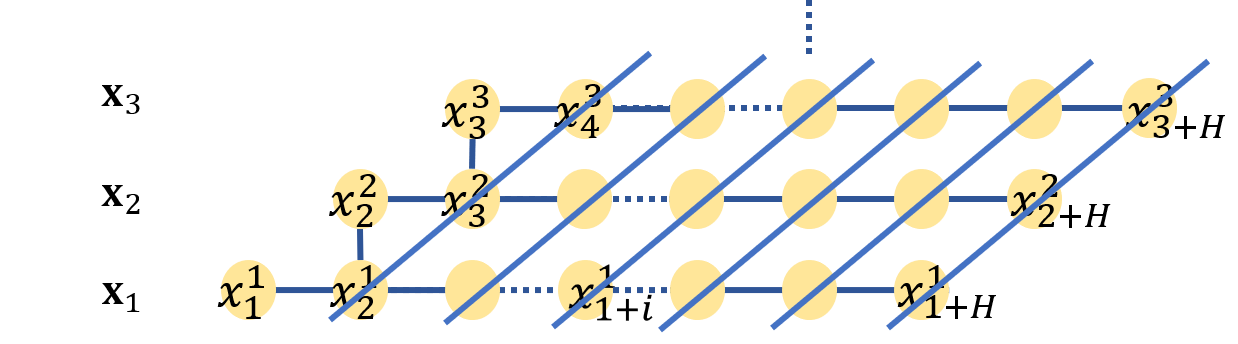
\includegraphics[width=8cm]{src/1_3_path.png}}\\
      \subfloat[Cost VS path.\label{fig:costplot}]{% This file was created by matlab2tikz.
%
%The latest updates can be retrieved from
%  http://www.mathworks.com/matlabcentral/fileexchange/22022-matlab2tikz-matlab2tikz
%where you can also make suggestions and rate matlab2tikz.
%
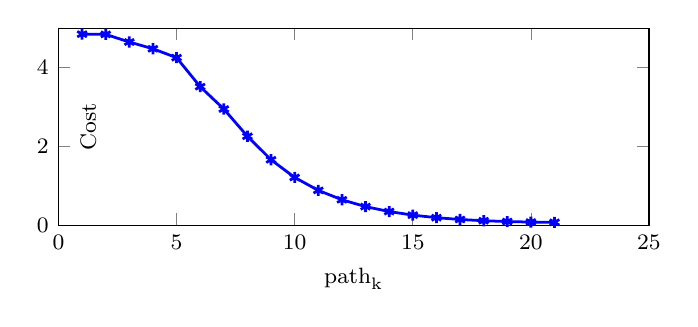
\begin{tikzpicture}

\begin{axis}[%
width=7.5cm,
height=2.5cm,
at={(3in,1in)},
scale only axis,
xmin=0,
xmax=25,
%xlabel style={font=\color{white!15!black}},
xlabel={$\text{path}_{\text{k}}$},
ymin=0,
ymax=5,
font = \footnotesize,
ylabel style={at={(0.08, 0.5)}},
ylabel={Cost},
axis background/.style={fill=white},
%title style={font=\bfseries},
%title={ Cost VS path},
legend style={legend cell align=left, align=left, draw=white!15!black}
]
\addplot [color=blue, line width=1.0pt, mark=asterisk, mark options={solid, blue}]
  table[row sep=crcr]
      
      \caption{Convergence of path cost.}
      
\end{figure}



\subsection{Result of scenario with initially unknown static obstacle}
In this scenario, the robot does not know all the obstacle location at the beginning, and has only limited ``eye sight," i.e., only the information of the environment within the range starting from 20 meters ahead to its current position. The robot is expected to execute this MPC motion planning and adjust it's planned trajectory to avoid collision once it ``sees" the obstacle.

The result of this scenario is shown in Fig.~\ref{fig:2_1}. At the beginning, the third obstacle on the right is unknown to the robot. After detecting the third obstacle, the robot corrects its planned trajectory to avoid the obstacle and completes its intention successfully.

The $M$-analysis discussed previously can also be applied to this scenario even though the environment is changing. Since the analysis strategy of this work focus on local conversions at each action locations, i.e., every point in the trajectories, the analysis can still be done although the planned locations change a lot due to environment changes. This directly demonstrate the strength of the proposed $M$-analysis. The result of $M$-analysis is shown in Fig.~\ref{fig:2_2}. From the plot we can see that $M$ begins to increase slower after the $16^{th}$ action location, this is exactly where the robot detects the obstacle and plans the new trajectory to avoid collision. The $26^{th}$ to the $30^{th}$ are the critical action locations, therefore, have higher $M$. After passing by the obstacle, the robot adjusts its planning to best lower the cost and then track the line with constant speed steadily. Throughout the process from detection to reaching 20-settling, the system is at least 14-settling. Once the environment stops changing, the robot system reaches to 20-settling, which agrees with the result from the static-obstacle-scenario.     




\begin{figure}[t]
      \centering
      \subfloat[Simulation result of scenario that has initially unknown static obstacle.\label{fig:2_1}]{% This file was created by matlab2tikz.
%
%The latest updates can be retrieved from
%  http://www.mathworks.com/matlabcentral/fileexchange/22022-matlab2tikz-matlab2tikz
%where you can also make suggestions and rate matlab2tikz.
%
\definecolor{mycolor1}{rgb}{0.98333,0.98333,0.98333}%
\definecolor{mycolor2}{rgb}{0.96667,0.96667,0.96667}%
\definecolor{mycolor3}{rgb}{0.93333,0.93333,0.93333}%
\definecolor{mycolor4}{rgb}{0.91667,0.91667,0.91667}%
\definecolor{mycolor5}{rgb}{0.33333,0.33333,0.33333}%
%
\begin{tikzpicture}

\begin{axis}[%
width=7.5cm,
height=3cm,
at={(3in,1in)},
scale only axis,
xmin=-10,
xmax=65,
%xlabel style={font=\color{white!15!black}},
xlabel={$x$[\si{\meter}]},
font = \footnotesize,
ymin=-11,
ymax=11,
ylabel style={at={(0.08, 0.5)}},
ylabel={$y$[\si{\meter}]},
axis background/.style={fill=white},
legend style={legend cell align=left, align=left, draw=white!15!black}
]

\addplot[area legend, line width=1.0pt, draw=black, fill=green, forget plot]
table[row sep=crcr] {%
x	y\\
3	2.1\\
6.8	2.1\\
5.8	-1\\
3.8	-1\\
}--cycle;

\addplot[area legend, line width=1.0pt, draw=black, fill=green, forget plot]
table[row sep=crcr] {%
x	y\\
23	0.1\\
26.8	0.1\\
26.8	-10\\
23	-10\\
}--cycle;
\addplot [color=mycolor1, mark=asterisk, mark options={solid, mycolor1}, forget plot]
  table[row sep=crcr]{%
-6	0\\
-4.30573668770685	-0.121230126216136\\
-2.87630513826835	-0.28418834756381\\
-1.46522555388652	-0.484790237321453\\
-0.0554176999716383	-0.723563785594289\\
1.35430202722899	-0.995883299879068\\
2.76401564753985	-1.2777178813988\\
4.17372884466345	-1.5\\
5.58344201246159	-1.5\\
6.99315517822756	-1.29295766765565\\
8.4028683438527	-1.03555026771578\\
9.81258150946808	-0.794624647748671\\
11.2222946750828	-0.59349103192322\\
12.6320078406974	-0.435624414091703\\
14.0417210063121	-0.316458735507208\\
15.4514341719267	-0.228997186341746\\
16.8611473375414	-0.166272084701486\\
18.2708605031561	-0.12223411313811\\
19.6805736687707	-0.0918639150066664\\
21.0902868343854	-0.0708643147212668\\
22.5	-0.0550302398687101\\
};


\addplot [color=blue, mark=o, mark options={solid, blue}, forget plot]
  table[row sep=crcr]{%
-4.30573668770685	-0.121230126216136\\
};
\addplot [color=mycolor2, mark=asterisk, mark options={solid, mycolor2}, forget plot]
  table[row sep=crcr]{%
-4.30573668770685	-0.121230126216136\\
-2.65651671917057	-0.266952161175341\\
-1.31114544737889	-0.464964150352054\\
0.013170114912306	-0.70749239953417\\
1.33602658619104	-0.985773136994679\\
2.65878194728953	-1.27354421516906\\
3.98153030178702	-1.5\\
5.30427817075024	-1.5\\
6.62702600606755	-1.29282873264247\\
7.94977383905331	-1.03520785774391\\
9.2725216718775	-0.793992794718195\\
10.5952695046905	-0.592481476028427\\
11.9180173375027	-0.434124066569769\\
13.2407651703149	-0.314323612051515\\
14.563513003127	-0.226055432324677\\
15.8862608359392	-0.162344804033397\\
17.2090086687514	-0.117193007923362\\
18.5317565015635	-0.0857635006292117\\
19.8545043343757	-0.0642212327973607\\
21.1772521671878	-0.0493865997739125\\
22.5	-0.0382227526693035\\
};
\addplot [color=blue, mark=o, mark options={solid, blue}, forget plot]
  table[row sep=crcr]{%
-2.65651671917057	-0.266952161175341\\
};
\addplot [color=white!95!black, mark=asterisk, mark options={solid, white!95!black}, forget plot]
  table[row sep=crcr]{%
-2.65651671917057	-0.266952161175341\\
-1.05114258111082	-0.44613497572038\\
0.21240322267365	-0.687325900883055\\
1.45226145371996	-0.971638946531279\\
2.69047821433809	-1.26738288773159\\
3.92858122648582	-1.5\\
5.16667635624085	-1.5\\
6.40477093977214	-1.29276530604793\\
7.64286548545193	-1.03503894564045\\
8.88096002850875	-0.793679847744095\\
10.1190545713838	-0.59197862529895\\
11.3571491142463	-0.433370836583504\\
12.5952436571078	-0.313239825476144\\
13.8333381999694	-0.224538782830126\\
15.0714327428309	-0.160273892455568\\
16.3095272856924	-0.114442475156813\\
17.5476218285539	-0.0822448936533275\\
18.7857163714154	-0.0599763048043718\\
20.023810914277	-0.0447841171138046\\
21.2619054571385	-0.0343551244244603\\
22.5	-0.0265185122240942\\
};
\addplot [color=blue, mark=o, mark options={solid, blue}, forget plot]
  table[row sep=crcr]{%
-1.05114258111082	-0.44613497572038\\
};
\addplot [color=mycolor3, mark=asterisk, mark options={solid, mycolor3}, forget plot]
  table[row sep=crcr]{%
-1.05114258111082	-0.44613497572038\\
0.947814819670018	-0.81134502698654\\
2.945869111991	-1.21686777768904\\
4.94386082188336	-1.5\\
6.94184819502056	-1.37599981301129\\
8.93983526763667	-1.10380804161612\\
10.9378223194521	-0.799469727853893\\
12.9358093701787	-0.507766240499674\\
14.9337964259187	-0.239822875139846\\
16.9317835554403	0.00674332366700078\\
18.9297717497832	0.235617871842776\\
20.9277753102518	0.441303293810504\\
22.9260006147228	0.594926657297048\\
24.927425841103	0.61951883609815\\
26.9289724786052	0.583602733701758\\
28.9290796554676	0.494471171211914\\
30.9290870824696	0.398992678773523\\
32.9290875971363	0.316138762996624\\
34.929087632801	0.251243584883324\\
36.9290876352733	0.202813736117701\\
38.9290876354565	0.165026293813502\\
};
\addplot [color=blue, mark=o, mark options={solid, blue}, forget plot]
  table[row sep=crcr]{%
0.947814819670018	-0.81134502698654\\
};
\addplot [color=mycolor4, mark=asterisk, mark options={solid, mycolor4}, forget plot]
  table[row sep=crcr]{%
0.947814819670018	-0.81134502698654\\
2.94723374530955	-1.19056291357689\\
4.94614933931302	-1.5\\
6.94503005409931	-1.38584799703101\\
8.94390835187264	-1.11578298813507\\
10.9427864821751	-0.810232153962354\\
12.941664601163	-0.516090613117848\\
14.9405427235599	-0.245446523172548\\
16.9394209067027	0.00366776350884273\\
18.9382999672517	0.234727319088293\\
20.9371916894455	0.44199646200136\\
22.9362661280816	0.596107938395995\\
24.9379772934867	0.619015838060864\\
26.9397561252479	0.580393907341798\\
28.9398793924043	0.4882001855657\\
30.9398879344105	0.389244711143201\\
32.9398885263432	0.302546636883444\\
34.9398885673622	0.233791580119787\\
36.9398885702047	0.182509335089464\\
38.9398885704017	0.145276522890386\\
40.9398885704163	0.116569014281613\\
};


\addplot [color=blue, mark=o, mark options={solid, blue}, forget plot]
  table[row sep=crcr]{%
2.94723374530955	-1.19056291357689\\
};
\addplot [color=white!90!black, mark=asterisk, mark options={solid, white!90!black}, forget plot]
  table[row sep=crcr]{%
2.94723374530955	-1.19056291357689\\
4.94695163354805	-1.5\\
6.94642515413918	-1.38578448503687\\
8.94588174086197	-1.11561753906816\\
10.9453371541412	-0.80993539271986\\
12.9447924863577	-0.515635799474801\\
14.9442478166075	-0.244811019731421\\
16.9437031994023	0.00449106933474043\\
18.943159346068	0.235701796196104\\
20.942626516316	0.442982254755956\\
22.9422527646352	0.59674331495702\\
24.9441746214064	0.618487034824828\\
26.9461293302121	0.578324508381646\\
28.9462647850658	0.484489354832561\\
30.9462741716391	0.383648368383868\\
32.9462748220975	0.294740959050428\\
34.9462748671721	0.223490906985536\\
36.9462748702956	0.169713623024239\\
38.9462748705121	0.130786356704104\\
40.9462748705271	0.103025685232069\\
42.9462748705282	0.0817921654039152\\
};
\addplot [color=blue, mark=o, mark options={solid, blue}, forget plot]
  table[row sep=crcr]{%
4.94695163354805	-1.5\\
};
\addplot [color=darkgray!5!mycolor4, mark=asterisk, mark options={solid, darkgray!5!mycolor4}, forget plot]
  table[row sep=crcr]{%
4.94695163354805	-1.5\\
6.94664469025044	-1.21470383616901\\
8.9460718700153	-0.905050683170402\\
10.9454806254061	-0.616417947359808\\
12.9448881043103	-0.359440709528344\\
14.9442954985333	-0.129760902088701\\
16.9437029413654	0.081302862826938\\
18.9431111737102	0.279611996928819\\
20.942530805381	0.460585453378963\\
22.9421149377656	0.596993746667083\\
24.9440729311739	0.616295537032931\\
26.9460666682596	0.578683000281083\\
28.946204827644	0.485076372836287\\
30.9462144016323	0.383301058378714\\
32.946215065078	0.292844298440329\\
34.9462151110526	0.219687558893756\\
36.9462151142384	0.16382010088551\\
38.9462151144592	0.122891448386582\\
40.9462151144745	0.0938295230783457\\
42.9462151144756	0.0733510378181918\\
44.9462151144757	0.0577729493336347\\
};
\addplot [color=blue, mark=o, mark options={solid, blue}, forget plot]
  table[row sep=crcr]{%
6.94664469025044	-1.21470383616901\\
};
\addplot [color=gray!12!mycolor4, mark=asterisk, mark options={solid, gray!12!mycolor4}, forget plot]
  table[row sep=crcr]{%
6.94664469025044	-1.21470383616901\\
8.94641692202166	-0.965267894629919\\
10.9459918590008	-0.689785927415296\\
12.9455531243545	-0.425643472049886\\
14.9451134459312	-0.18140652561228\\
16.9446737543677	0.0456883339575248\\
18.9442348160474	0.258903811566242\\
20.9438068128941	0.452278504442167\\
22.9435366164178	0.596985426868887\\
24.9455436815925	0.617249782683278\\
26.9475772704741	0.577984984343555\\
28.9477181914561	0.483477378654109\\
30.947727956814	0.38107573216735\\
32.947728633521	0.290007922104333\\
34.9477286804145	0.216114957289613\\
36.9477286836641	0.159324873066676\\
38.9477286838893	0.117311397210423\\
40.9477286839049	0.087170318025758\\
42.947728683906	0.0660680522928613\\
44.947728683906	0.0513319076165083\\
46.947728683906	0.0401688495151028\\
};
\addplot [color=blue, mark=o, mark options={solid, blue}, forget plot]
  table[row sep=crcr]{%
8.94641692202166	-0.965267894629919\\
};
\addplot [color=white!85!black, mark=asterisk, mark options={solid, white!85!black}, forget plot]
  table[row sep=crcr]{%
8.94641692202166	-0.965267894629919\\
10.9461678406125	-0.740314302686911\\
12.9457030029846	-0.48609261853155\\
14.945223217798	-0.234161784682464\\
16.9447424492299	0.00707846211515625\\
18.944262369187	0.235591180824513\\
20.9437932561426	0.442621743258917\\
22.9434824760509	0.596894884052978\\
24.9454565567754	0.618625539858187\\
26.9474596431353	0.577904987296564\\
28.9475984503935	0.482667622153166\\
30.9476080692773	0.37984235177019\\
32.9476087358342	0.288430749762385\\
34.9476087820243	0.214149106343575\\
36.9476087852252	0.156857153533965\\
38.947608785447	0.11420201334118\\
40.9476087854623	0.0833063564045567\\
42.9476087854634	0.0614624943244575\\
44.9476087854635	0.0463233183092771\\
46.9476087854635	0.035820937883647\\
48.9476087854635	0.0278896944515099\\
};
\addplot [color=blue, mark=o, mark options={solid, blue}, forget plot]
  table[row sep=crcr]{%
10.9461678406125	-0.740314302686911\\
};
\addplot [color=gray!20!mycolor4, mark=asterisk, mark options={solid, gray!20!mycolor4}, forget plot]
  table[row sep=crcr]{%
10.9461678406125	-0.740314302686911\\
12.9458715905997	-0.52870641406243\\
14.9453187299428	-0.283377346233429\\
16.9447481401062	-0.0331139540022462\\
18.9441770878074	0.209932937341541\\
20.9436170589878	0.431659949764771\\
22.9432173330777	0.596807118906925\\
24.945130975877	0.62024156127871\\
26.9470791171054	0.577940807717131\\
28.9472141168477	0.482002713279988\\
30.9472234718833	0.378872393852647\\
32.9472241201563	0.287298717161373\\
34.9472241650795	0.212865252607834\\
36.9472241681925	0.155360739804499\\
38.9472241684082	0.112395131608544\\
40.9472241684232	0.0810797961906124\\
42.9472241684242	0.0587314815299306\\
44.9472241684243	0.0430964561748202\\
46.9472241684243	0.0323410592498915\\
48.9472241684243	0.0249166212861049\\
50.9472241684243	0.0193228993324973\\
};


\addplot [color=blue, mark=o, mark options={solid, blue}, forget plot]
  table[row sep=crcr]{%
12.9458715905997	-0.52870641406243\\
};
\addplot [color=darkgray!15!mycolor4, mark=asterisk, mark options={solid, darkgray!15!mycolor4}, forget plot]
  table[row sep=crcr]{%
12.9458715905997	-0.52870641406243\\
14.9451985365373	-0.3196306618581\\
16.9439425389186	-0.0723631852295447\\
18.9426470355146	0.181827259450315\\
20.9413616417801	0.418751559095684\\
22.9402623440377	0.596496165131011\\
24.9418513285124	0.622620104220936\\
26.9435186897847	0.579263116929798\\
28.9436342324049	0.482693476192677\\
30.9436422391263	0.379162423096829\\
32.9436427939656	0.287305818740509\\
34.9436428324142	0.212638627436899\\
36.9436428350785	0.154905229088508\\
38.9436428352632	0.111684968703611\\
40.943642835276	0.0800684988178036\\
42.9436428352768	0.0573641187810465\\
44.9436428352769	0.0413327479269348\\
46.9436428352769	0.0302036042413337\\
48.9436428352769	0.0225903818980173\\
50.9436428352769	0.0173545555298355\\
52.9436428352769	0.013416778662304\\
};
\addplot [color=blue, mark=o, mark options={solid, blue}, forget plot]
  table[row sep=crcr]{%
14.9451985365373	-0.3196306618581\\
};
\addplot [color=white!80!black, mark=asterisk, mark options={solid, white!80!black}, forget plot]
  table[row sep=crcr]{%
14.9451985365373	-0.3196306618581\\
16.944326279901	-0.102833315855688\\
18.9426994458641	0.153297750382067\\
20.9410344474729	0.404506109999756\\
22.9395706433443	0.596409095312835\\
24.9410623203771	0.624746045984467\\
26.9426555593661	0.579355192905859\\
28.9427659655573	0.481973563314904\\
30.9427736163411	0.378200059370587\\
32.9427741465151	0.286338967889468\\
34.9427741832544	0.211740778951174\\
36.9427741858004	0.154070485512274\\
38.9427741859768	0.110869989331473\\
40.942774185989	0.0792125665209127\\
42.9427741859898	0.0563995304112827\\
44.9427741859899	0.0401937593576906\\
46.9427741859899	0.0288417877226991\\
48.9427741859899	0.0210073616102868\\
50.9427741859899	0.0156709104995867\\
52.9427741859899	0.0120114832900739\\
54.9427741859899	0.00926309530683742\\
};
\addplot [color=blue, mark=o, mark options={solid, blue}, forget plot]
  table[row sep=crcr]{%
16.944326279901	-0.102833315855688\\
};
\addplot [color=darkgray!20!mycolor4, mark=asterisk, mark options={solid, darkgray!20!mycolor4}, forget plot]
  table[row sep=crcr]{%
16.944326279901	-0.102833315855688\\
18.9431407569108	0.128673991815372\\
20.9409440501817	0.388361229479561\\
22.9389042166147	0.596310938700271\\
24.9401502276384	0.62731883534518\\
26.9415340274567	0.579797846445256\\
28.9416299202062	0.48153051605228\\
30.9416365652565	0.377464414998988\\
32.9416370257365	0.28557120298535\\
34.9416370576463	0.211035763481208\\
36.9416370598575	0.153443306061891\\
38.9416370600108	0.110298743171075\\
40.9416370600214	0.0786587692135949\\
42.9416370600221	0.0558174359023984\\
44.9416370600222	0.0395351768128955\\
46.9416370600222	0.0280610908362228\\
48.9416370600222	0.0200716045792873\\
50.9416370600222	0.0145823899670535\\
52.9416370600222	0.0108556745178722\\
54.9416370600222	0.00830581583326776\\
56.9416370600222	0.0063928161711595\\
};
\addplot [color=blue, mark=o, mark options={solid, blue}, forget plot]
  table[row sep=crcr]{%
18.9431407569108	0.128673991815372\\
};
\addplot [color=gray!36!mycolor4, mark=asterisk, mark options={solid, gray!36!mycolor4}, forget plot]
  table[row sep=crcr]{%
18.9431407569108	0.128673991815372\\
20.9417923449589	0.372509100660308\\
22.9395169944582	0.596330426847445\\
24.9406561844006	0.629574286934603\\
26.9419479462995	0.579519708764522\\
28.9420374611257	0.480317787369886\\
30.9420436642071	0.376054745064965\\
32.9420440940601	0.284270354340394\\
34.9420441238475	0.209940976223734\\
36.9420441259117	0.152556960329485\\
38.9420441260547	0.109584288572163\\
40.9420441260647	0.0780667669182742\\
42.9420441260654	0.0552965619574338\\
44.9420441260654	0.0390361602798664\\
46.9420441260654	0.0275381220195619\\
48.9420441260654	0.0194843810051483\\
50.9420441260655	0.0139021135872207\\
52.9420441260655	0.01008001386436\\
54.9420441260655	0.00749175410331937\\
56.9420441260655	0.00572392585854391\\
58.9420441260655	0.0043987487374454\\
};
\addplot [color=blue, mark=o, mark options={solid, blue}, forget plot]
  table[row sep=crcr]{%
20.9417923449589	0.372509100660308\\
};
\addplot [color=lightgray, mark=asterisk, mark options={solid, lightgray}, forget plot]
  table[row sep=crcr]{%
20.9417923449589	0.372509100660308\\
22.9398853455116	0.596381601037896\\
24.9410307402831	0.629579059476723\\
26.9423048635693	0.579457984110389\\
28.942393156098	0.480236664937572\\
30.9423992744781	0.375973800464111\\
32.9423996984616	0.28419548329865\\
34.9423997278422	0.209871389680634\\
36.9423997298782	0.152488533458297\\
38.9423997300193	0.109510977693679\\
40.9423997300291	0.0779810090047666\\
42.9423997300297	0.0551891586627134\\
44.9423997300297	0.0388959666618652\\
46.9423997300297	0.0273518442340341\\
48.9423997300297	0.0192369390644474\\
50.9423997300297	0.0135784152557529\\
52.9423997300297	0.00966978063782195\\
54.9423997300296	0.00700056687311991\\
56.9423997300296	0.00519652701883541\\
58.9423997300296	0.00396597274370978\\
60.9423997300296	0.00304413215512191\\
};
\addplot [color=blue, mark=o, mark options={solid, blue}, forget plot]
  table[row sep=crcr]{%
22.9398853455116	0.596381601037896\\
};

\addplot[area legend, line width=1.0pt, draw=black, fill=green, forget plot]
table[row sep=crcr] {%
x	y\\
43	10\\
49.8	10\\
49.8	-1\\
43.5	-1\\
}--cycle;
\addplot [color=black!20!mycolor4, mark=asterisk, mark options={solid, black!20!mycolor4}, forget plot]
  table[row sep=crcr]{%
22.9398853455116	0.596381601037896\\
24.9427030343211	0.60314119204023\\
26.9476333084854	0.577804756588279\\
28.9479749601747	0.438691417926482\\
30.9479986355066	0.255612658346385\\
32.9480002761287	0.054462678784065\\
34.9480003898184	-0.160680562732834\\
36.9480003976967	-0.395458873093158\\
38.9480003982426	-0.657297565470826\\
40.9480003982804	-0.947379200393772\\
42.948000398283	-1.24814293138903\\
44.9480003982832	-1.50000000000009\\
46.9480003982833	-1.55650117000911\\
48.9480003982833	-1.5000000000001\\
50.9480003982833	-1.27852382004827\\
52.9480003982833	-1.02721088669519\\
54.9480003982833	-0.802354888779395\\
56.9480003982833	-0.622117438523328\\
58.9480003982833	-0.486851677540312\\
60.9480003982833	-0.388290720154033\\
62.9480003982833	-0.312177498609529\\
};
\addplot [color=blue, mark=o, mark options={solid, blue}, forget plot]
  table[row sep=crcr]{%
24.9427030343211	0.60314119204023\\
};
\addplot [color=darkgray!30!mycolor4, mark=asterisk, mark options={solid, darkgray!30!mycolor4}, forget plot]
  table[row sep=crcr]{%
24.9427030343211	0.60314119204023\\
26.9457172580495	0.578295798015645\\
28.9459261337206	0.439319476250036\\
30.9459406080519	0.256229389332701\\
32.9459416110135	0.055019843464577\\
34.9459416804537	-0.160186054095426\\
36.9459416852039	-0.395014364107568\\
38.9459416854714	-0.656893050853408\\
40.9459416854285	-0.947024548775977\\
42.9459416853681	-1.247893045364\\
44.9459416853639	-1.50000000000013\\
46.9459416853637	-1.5570714491935\\
48.9459416853637	-1.5000000000002\\
50.9459416853637	-1.27475323782431\\
52.9459416853637	-1.01782004506852\\
54.9459416853637	-0.786108426954408\\
56.9459416853637	-0.598246173770949\\
58.9459416853637	-0.455480336924727\\
60.9459416853637	-0.351693867302397\\
62.9459416853637	-0.277485382556323\\
64.9459416853637	-0.220657799411877\\
};
\addplot [color=blue, mark=o, mark options={solid, blue}, forget plot]
  table[row sep=crcr]{%
26.9457172580495	0.578295798015645\\
};
\addplot [color=white!70!black, mark=asterisk, mark options={solid, white!70!black}, forget plot]
  table[row sep=crcr]{%
26.9457172580495	0.578295798015645\\
28.9457172580495	0.418496727815201\\
30.9457172580495	0.230615840272563\\
32.9457172580495	0.031505108083899\\
34.9457172580495	-0.17912921039126\\
36.9457172580495	-0.40891790534083\\
38.9457172580495	-0.666112494670364\\
40.9457172580495	-0.952221548208361\\
42.9457172580495	-1.24990524315403\\
44.9457172580495	-1.5\\
46.9457172580495	-1.55705250803135\\
48.9457172580495	-1.5\\
50.9457172580495	-1.27287457522497\\
52.9457172580495	-1.0129336535084\\
54.9457172580495	-0.777383177420373\\
56.9457172580495	-0.584977629669864\\
58.9457172580495	-0.437174798263567\\
60.9457172580495	-0.328484947896797\\
62.9457172580495	-0.251116093871448\\
64.9457172580495	-0.19651250226529\\
66.9457172580495	-0.154945265672115\\
};
\addplot [color=blue, mark=o, mark options={solid, blue}, forget plot]
  table[row sep=crcr]{%
28.9457172580495	0.418496727815201\\
};
\addplot [color=darkgray!35!mycolor4, mark=asterisk, mark options={solid, darkgray!35!mycolor4}, forget plot]
  table[row sep=crcr]{%
28.9457172580495	0.418496727815201\\
30.9457172580496	0.26103075814587\\
32.9457172580496	0.0685822198501429\\
34.9457172580496	-0.145641293084201\\
36.9457172580496	-0.3827487849812\\
38.9457172580496	-0.648009184992007\\
40.9457172580496	-0.941630437075622\\
42.9457172580496	-1.24560045197784\\
44.9457172580496	-1.5\\
46.9457172580496	-1.55784459540449\\
48.9457172580496	-1.5\\
50.9457172580496	-1.27159515043971\\
52.9457172580496	-1.01000054196475\\
54.9457172580496	-0.772412032836895\\
56.9457172580496	-0.577528503893271\\
58.9457172580496	-0.426780724421257\\
60.9457172580496	-0.314790913249377\\
62.9457172580496	-0.234221237135159\\
64.9457172580496	-0.177704384702491\\
66.9457172580496	-0.138188394559281\\
68.9457172580496	-0.10823651722304\\
};
\addplot [color=blue, mark=o, mark options={solid, blue}, forget plot]
  table[row sep=crcr]{%
30.9457172580496	0.26103075814587\\
};
\addplot [color=gray!60!mycolor4, mark=asterisk, mark options={solid, gray!60!mycolor4}, forget plot]
  table[row sep=crcr]{%
30.9457172580496	0.26103075814587\\
32.9457172580496	0.0962876021708383\\
34.9457172580496	-0.112495528512046\\
36.9457172580496	-0.353821398085587\\
38.9457172580496	-0.626839363752318\\
40.9457172580496	-0.928853760857085\\
42.9457172580496	-1.24032517227614\\
44.9457172580496	-1.50000000000001\\
46.9457172580496	-1.55871009555787\\
48.9457172580496	-1.50000000000002\\
50.9457172580497	-1.27076865415868\\
52.9457172580497	-1.00828334222462\\
54.9457172580497	-0.769645932634311\\
56.9457172580497	-0.573468077884848\\
58.9457172580497	-0.421108911262053\\
60.9457172580497	-0.307163506220837\\
62.9457172580497	-0.224378371443793\\
64.9457172580497	-0.165721975434564\\
66.9457172580497	-0.125008237508507\\
68.9457172580497	-0.0967363072508379\\
70.9457172580497	-0.0753758262055403\\
};


\addplot [color=blue, mark=o, mark options={solid, blue}, forget plot]
  table[row sep=crcr]{%
32.9457172580496	0.0962876021708383\\
};
\addplot [color=white!65!black, mark=asterisk, mark options={solid, white!65!black}, forget plot]
  table[row sep=crcr]{%
32.9457172580496	0.0962876021708383\\
34.9457172580496	-0.0862172385143777\\
36.9457172580496	-0.323479944471226\\
38.9457172580496	-0.602074031338828\\
40.9457172580495	-0.91306470798812\\
42.9457172580495	-1.23361177661394\\
44.9457172580495	-1.5\\
46.9457172580495	-1.55975412947941\\
48.9457172580495	-1.5\\
50.9457172580495	-1.27012161055854\\
52.9457172580495	-1.00713044113224\\
54.9457172580496	-0.767975501177934\\
56.9457172580496	-0.571167392831865\\
58.9457172580496	-0.417991358975491\\
60.9457172580496	-0.302990310093519\\
62.9457172580496	-0.218895081209088\\
64.9457172580496	-0.158739901839429\\
66.9457172580496	-0.116584272198706\\
68.9457172580496	-0.087550472273578\\
70.9457172580496	-0.0674924832985665\\
72.9457172580496	-0.0523746683695731\\
};
\addplot [color=blue, mark=o, mark options={solid, blue}, forget plot]
  table[row sep=crcr]{%
34.9457172580496	-0.0862172385143777\\
};
\addplot [color=gray!68!mycolor4, mark=asterisk, mark options={solid, gray!68!mycolor4}, forget plot]
  table[row sep=crcr]{%
34.9457172580496	-0.0862172385143777\\
36.9457172580495	-0.29755714363535\\
38.9457172580495	-0.574128688481032\\
40.9457172580495	-0.893231522896236\\
42.9457172580495	-1.22472450708648\\
44.9457172580495	-1.5\\
46.9457172580495	-1.56110538959235\\
48.9457172580495	-1.5\\
50.9457172580495	-1.26948249631751\\
52.9457172580495	-1.0061618995294\\
54.9457172580495	-0.766771559251552\\
56.9457172580495	-0.569701858378487\\
58.9457172580495	-0.416164921544543\\
60.9457172580495	-0.300654162484696\\
62.9457172580495	-0.215867837743744\\
64.9457172580495	-0.154833712901695\\
66.9457172580495	-0.111662261600824\\
68.9457172580495	-0.0816536086089081\\
70.9457172580495	-0.0611061647681606\\
72.9457172580495	-0.0469662650659349\\
74.9457172580495	-0.0363287083204365\\
};
\addplot [color=blue, mark=o, mark options={solid, blue}, forget plot]
  table[row sep=crcr]{%
36.9457172580495	-0.29755714363535\\
};
\addplot [color=darkgray!50!mycolor1, mark=asterisk, mark options={solid, darkgray!50!mycolor1}, forget plot]
  table[row sep=crcr]{%
36.9457172580495	-0.29755714363535\\
38.9457172580496	-0.548103995874345\\
40.9457172580496	-0.868896439509084\\
42.9457172580496	-1.21262423571996\\
44.9457172580496	-1.5\\
46.9457172580496	-1.56292912009079\\
48.9457172580496	-1.5\\
50.9457172580496	-1.26872546763997\\
52.9457172580496	-1.0051345666749\\
54.9457172580496	-0.765661883084489\\
56.9457172580497	-0.56854438320201\\
58.9457172580497	-0.414913531060478\\
60.9457172580497	-0.299216895403285\\
62.9457172580497	-0.214123476662963\\
64.9457172580497	-0.152643038960321\\
66.9457172580497	-0.108885663101855\\
68.9457172580497	-0.0781908088681367\\
70.9457172580497	-0.0569849136970165\\
72.9457172580497	-0.0425293541142381\\
74.9457172580497	-0.0326114287548648\\
76.9457172580497	-0.025160785659951\\
};
\addplot [color=blue, mark=o, mark options={solid, blue}, forget plot]
  table[row sep=crcr]{%
38.9457172580496	-0.548103995874345\\
};
\addplot [color=white!60!black, mark=asterisk, mark options={solid, white!60!black}, forget plot]
  table[row sep=crcr]{%
38.9457172580496	-0.548103995874345\\
40.9457172580495	-0.843959297554692\\
42.9457172580495	-1.1963603136356\\
44.9457172580495	-1.5\\
46.9457172580495	-1.56537263199079\\
48.9457172580495	-1.5\\
50.9457172580495	-1.26776263082935\\
52.9457172580495	-1.00389498022226\\
54.9457172580495	-0.764428231662428\\
56.9457172580495	-0.567399270646097\\
58.9457172580495	-0.413842464858124\\
60.9457172580495	-0.298158296065245\\
62.9457172580495	-0.212991441288835\\
64.9457172580495	-0.151337319755243\\
66.9457172580495	-0.107298145247786\\
68.9457172580495	-0.076216739075082\\
70.9457172580495	-0.0545498994507411\\
72.9457172580495	-0.0396508709087984\\
74.9457172580495	-0.0295293085519518\\
76.9457172580495	-0.0226010570300069\\
78.9457172580495	-0.0174021509826229\\
};
\addplot [color=blue, mark=o, mark options={solid, blue}, forget plot]
  table[row sep=crcr]{%
40.9457172580495	-0.843959297554692\\
};
\addplot [color=darkgray!50!mycolor4, mark=asterisk, mark options={solid, darkgray!50!mycolor4}, forget plot]
  table[row sep=crcr]{%
40.9457172580495	-0.843959297554692\\
42.9457172580496	-1.17766400642021\\
44.9457172580496	-1.5\\
46.9457172580496	-1.56817865061168\\
48.9457172580496	-1.5\\
50.9457172580496	-1.2666765067678\\
52.9457172580496	-1.00252361836127\\
54.9457172580496	-0.763108259301063\\
56.9457172580496	-0.566239937862917\\
58.9457172580496	-0.412846268168552\\
60.9457172580497	-0.29728019331843\\
62.9457172580497	-0.21216614042671\\
64.9457172580497	-0.150490537920829\\
66.9457172580497	-0.106350732399807\\
68.9457172580497	-0.075087442059055\\
70.9457172580497	-0.0531621060641259\\
72.9457172580497	-0.0379507686505322\\
74.9457172580497	-0.0275283680412478\\
76.9457172580497	-0.0204667724288746\\
78.9457172580497	-0.0156418341024076\\
80.9457172580497	-0.0120243953723512\\
};
\addplot [color=blue, mark=o, mark options={solid, blue}, forget plot]
  table[row sep=crcr]{%
42.9457172580496	-1.17766400642021\\
};
\addplot [color=gray!84!mycolor4, mark=asterisk, mark options={solid, gray!84!mycolor4}, forget plot]
  table[row sep=crcr]{%
42.9457172580496	-1.17766400642021\\
44.9457172580496	-1.5\\
46.9457172580496	-1.56817968627602\\
48.9457172580496	-1.5\\
50.9457172580496	-1.26666920533388\\
52.9457172580496	-1.00250463890986\\
54.9457172580495	-0.763073291214543\\
56.9457172580495	-0.566183530153349\\
58.9457172580495	-0.41276085238805\\
60.9457172580495	-0.297155119720696\\
62.9457172580495	-0.211986623882907\\
64.9457172580495	-0.150236519035052\\
66.9457172580495	-0.105995823638318\\
68.9457172580495	-0.0745984349277023\\
70.9457172580495	-0.0525001122993462\\
72.9457172580495	-0.0370762264441343\\
74.9457172580495	-0.0264143608245566\\
76.9457172580495	-0.0191292976987131\\
78.9457172580495	-0.0142035025303436\\
80.9457172580495	-0.0108426098769887\\
82.9457172580495	-0.00832453042717946\\
};
\addplot [color=blue, mark=o, mark options={solid, blue}, forget plot]
  table[row sep=crcr]{%
44.9457172580496	-1.5\\
};
\addplot [color=white!55!black, mark=asterisk, mark options={solid, white!55!black}, forget plot]
  table[row sep=crcr]{%
44.9457172580496	-1.5\\
46.9457172580496	-1.5214479496814\\
48.9457172580496	-1.5\\
50.9457172580496	-1.28451592958693\\
52.9457172580496	-1.02469723793357\\
54.9457172580496	-0.783852317431852\\
56.9457172580496	-0.583541584152807\\
58.9457172580496	-0.426399931907231\\
60.9457172580496	-0.307469715815008\\
62.9457172580496	-0.219579012477341\\
64.9457172580497	-0.155702169081957\\
66.9457172580497	-0.109841512163857\\
68.9457172580497	-0.0772223530425895\\
70.9457172580497	-0.0541986763279236\\
72.9457172580497	-0.0380610901808007\\
74.9457172580497	-0.0268333142295375\\
76.9457172580497	-0.0190909186913404\\
78.9457172580497	-0.0138104982784718\\
80.9457172580497	-0.0102450893312917\\
82.9457172580497	-0.00781470900908038\\
84.9457172580497	-0.00599463431703825\\
};
\addplot [color=blue, mark=o, mark options={solid, blue}, forget plot]
  table[row sep=crcr]{%
46.9457172580496	-1.5214479496814\\
};
\addplot [color=gray!92!mycolor4, mark=asterisk, mark options={solid, gray!92!mycolor4}, forget plot]
  table[row sep=crcr]{%
46.9457172580496	-1.5214479496814\\
48.9457172580495	-1.50000000001292\\
50.9457172580495	-1.28451425722739\\
52.9457172580495	-1.02469275235459\\
54.9457172580495	-0.783843922519279\\
56.9457172580495	-0.583527904747255\\
58.9457172580495	-0.426379045969976\\
60.9457172580495	-0.307438877378917\\
62.9457172580494	-0.219534322960164\\
64.9457172580494	-0.155638169917009\\
66.9457172580494	-0.109750689992534\\
68.9457172580494	-0.0770945829933127\\
70.9457172580494	-0.0540207006889178\\
72.9457172580494	-0.0378162780466697\\
74.9457172580494	-0.0265022448305165\\
76.9457172580493	-0.0186539116151203\\
78.9457172580493	-0.0132543267339956\\
80.9457172580493	-0.00957821710703694\\
82.9457172580493	-0.00709933094452191\\
84.9457172580493	-0.00541111733359818\\
86.9457172580493	-0.00414739508998293\\
};
\addplot [color=blue, mark=o, mark options={solid, blue}, forget plot]
  table[row sep=crcr]{%
48.9457172580495	-1.50000000001292\\
};
\addplot [color=darkgray!60!mycolor4, mark=asterisk, mark options={solid, darkgray!60!mycolor4}, forget plot]
  table[row sep=crcr]{%
48.9457172580495	-1.50000000001292\\
50.9457172580496	-1.24377024594653\\
52.9457172580496	-0.974015343637389\\
54.9457172580496	-0.736373935457746\\
56.9457172580496	-0.543840643662734\\
58.9457172580496	-0.39514545192691\\
60.9457172580496	-0.283745361771292\\
62.9457172580496	-0.201987652910655\\
64.9457172580496	-0.142853527618699\\
66.9457172580496	-0.100536597307932\\
68.9457172580496	-0.0704963945005217\\
70.9457172580496	-0.0493039856049175\\
72.9457172580496	-0.0344295142604457\\
74.9457172580496	-0.0240368936017532\\
76.9457172580496	-0.0168094863933541\\
78.9457172580496	-0.0118114174448213\\
80.9457172580496	-0.00838100637599359\\
82.9457172580496	-0.00604983087432089\\
84.9457172580496	-0.00448003609203111\\
86.9457172580496	-0.00341196599732752\\
88.9457172580496	-0.00261282509760496\\
};
\addplot [color=blue, mark=o, mark options={solid, blue}, forget plot]
  table[row sep=crcr]{%
50.9457172580496	-1.24377024594653\\
};
\addplot [color=gray, mark=asterisk, mark options={solid, gray}, forget plot]
  table[row sep=crcr]{%
50.9457172580496	-1.24377024594653\\
52.9457172580532	-1.03130961645886\\
54.9457172580595	-0.807634202333864\\
56.9457172580651	-0.610586660536463\\
58.9457172580696	-0.450941874078691\\
60.9457172580735	-0.327646770615573\\
62.9457172580769	-0.235276025595526\\
64.94571725808	-0.167484155157726\\
66.945717258083	-0.118451311452697\\
68.9457172580859	-0.0833629522394646\\
70.9457172580887	-0.0584542119503189\\
72.9457172580913	-0.0408818868676205\\
74.9457172580939	-0.028548270279439\\
76.9457172580963	-0.019930915377722\\
78.9457172580984	-0.0139380926836776\\
80.9457172580998	-0.00979379305346474\\
82.9457172581006	-0.00694936424097424\\
84.945717258101	-0.00501639975628485\\
86.9457172581011	-0.00371475706132717\\
88.9457172581011	-0.00282913452508353\\
90.9457172581011	-0.00216650274282709\\
};
\addplot [color=blue, mark=o, mark options={solid, blue}, forget plot]
  table[row sep=crcr]{%
52.9457172580532	-1.03130961645886\\
};
\addplot [color=black!50!mycolor2, mark=asterisk, mark options={solid, black!50!mycolor2}, forget plot]
  table[row sep=crcr]{%
52.9457172580532	-1.03130961645886\\
54.9457172580589	-0.855141476865846\\
56.9457172580695	-0.669674260308516\\
58.9457172580801	-0.506286347293614\\
60.9457172580898	-0.373912057083673\\
62.9457172580981	-0.271678202979025\\
64.9457172581051	-0.195086213478469\\
66.9457172581111	-0.1388745392339\\
68.9457172581165	-0.0982174778512837\\
70.9457172581215	-0.0691229064058715\\
72.9457172581261	-0.0484690730489532\\
74.9457172581304	-0.0338984496557739\\
76.9457172581342	-0.0236716594310012\\
78.9457172581374	-0.0165263196807186\\
80.9457172581396	-0.011557189976705\\
82.9457172581409	-0.00812081892983778\\
84.9457172581415	-0.00576227498073282\\
86.9457172581417	-0.00415949917239512\\
88.9457172581419	-0.00308020286917688\\
90.9457172581419	-0.00234586222937059\\
92.9457172581419	-0.00179642109951628\\
};
\addplot [color=blue, mark=o, mark options={solid, blue}, forget plot]
  table[row sep=crcr]{%
54.9457172580589	-0.855141476865846\\
};
\addplot [color=black!50!mycolor3, mark=asterisk, mark options={solid, black!50!mycolor3}, forget plot]
  table[row sep=crcr]{%
54.9457172580589	-0.855141476865846\\
56.9457172580561	-0.70906634999357\\
58.9457172580509	-0.55528061295935\\
60.9457172580456	-0.419802596456574\\
62.9457172580405	-0.310040460796222\\
64.9457172580361	-0.225270176887494\\
66.9457172580322	-0.161761618475435\\
68.9457172580283	-0.115152013208897\\
70.9457172580245	-0.081439984385571\\
72.9457172580208	-0.0573153428641627\\
74.9457172580172	-0.0401895939349147\\
76.9457172580138	-0.0281079220408015\\
78.9457172580105	-0.0196280704454803\\
80.9457172580072	-0.0137032964598286\\
82.9457172580041	-0.00958299267714982\\
84.9457172580013	-0.00673362196911062\\
86.9457172579994	-0.00477796411070953\\
88.9457172579978	-0.00344897420318038\\
90.9457172579966	-0.00255404311753089\\
92.9457172579958	-0.0019451424254241\\
94.9457172579953	-0.00148955673929286\\
};
\addplot [color=blue, mark=o, mark options={solid, blue}, forget plot]
  table[row sep=crcr]{%
56.9457172580561	-0.70906634999357\\
};
\addplot [color=white!45!black, mark=asterisk, mark options={solid, white!45!black}, forget plot]
  table[row sep=crcr]{%
56.9457172580561	-0.70906634999357\\
58.9457172580552	-0.587943752343709\\
60.9457172580536	-0.460427669695565\\
62.9457172580519	-0.348091985759341\\
64.9457172580503	-0.257079400116307\\
66.9457172580487	-0.186789562206245\\
68.945717258047	-0.134129525329495\\
70.9457172580456	-0.09548176519263\\
72.9457172580441	-0.0675284196055818\\
74.9457172580422	-0.0475247453934479\\
76.9457172580399	-0.0333244140883939\\
78.9457172580373	-0.0233065314063427\\
80.9457172580347	-0.0162752066701882\\
82.9457172580321	-0.0113625016053448\\
84.94571725803	-0.00794602743926172\\
86.9457172580284	-0.00558338576839085\\
88.945717258027	-0.00396179306471742\\
90.9457172580258	-0.00285982099529776\\
92.9457172580249	-0.00211776189097312\\
94.9457172580242	-0.00161287351526337\\
96.9457172580238	-0.00123511090134512\\
};
\addplot [color=blue, mark=o, mark options={solid, blue}, forget plot]
  table[row sep=crcr]{%
58.9457172580552	-0.587943752343709\\
};
\addplot [color=darkgray!75!mycolor1, mark=asterisk, mark options={solid, darkgray!75!mycolor1}, forget plot]
  table[row sep=crcr]{%
58.9457172580552	-0.587943752343709\\
60.9457172580575	-0.487511296965882\\
62.9457172580618	-0.381777490648941\\
64.9457172580662	-0.288630969824832\\
66.9457172580706	-0.213165139139471\\
68.9457172580749	-0.15488219981691\\
70.9457172580792	-0.111217541805624\\
72.9457172580833	-0.079171585718883\\
74.9457172580871	-0.0559932260419497\\
76.9457172580905	-0.039406576179047\\
78.9457172580932	-0.0276319431393168\\
80.9457172580951	-0.0193253135345358\\
82.9457172580964	-0.0134950785369897\\
84.9457172580971	-0.00942156094585527\\
86.9457172580975	-0.00658868833666598\\
88.9457172580978	-0.00462963272863513\\
90.945717258098	-0.00328504022472217\\
92.9457172580981	-0.00237130684351394\\
94.9457172580981	-0.00175600615371381\\
96.9457172580981	-0.00133736272755383\\
98.9457172580981	-0.0010241294614008\\
};
\addplot [color=blue, mark=o, mark options={solid, blue}, forget plot]
  table[row sep=crcr]{%
60.9457172580575	-0.487511296965882\\
};
\addplot [color=darkgray!75!mycolor4, mark=asterisk, mark options={solid, darkgray!75!mycolor4}, forget plot]
  table[row sep=crcr]{%
60.9457172580575	-0.487511296965882\\
62.9457172580576	-0.404234697149085\\
64.9457172580577	-0.316562322291398\\
66.9457172580579	-0.239327074882433\\
68.945717258058	-0.176752305021589\\
70.9457172580582	-0.128425247838207\\
72.9457172580583	-0.0922193795492787\\
74.9457172580584	-0.0656475084271139\\
76.9457172580586	-0.0464284723499389\\
78.9457172580587	-0.0326751512971196\\
80.9457172580587	-0.0229118591427028\\
82.9457172580588	-0.0160241666450807\\
84.9457172580589	-0.011189851433908\\
86.9457172580589	-0.00781217144980982\\
88.9457172580589	-0.00546320967525312\\
90.9457172580589	-0.00383879962498524\\
92.945717258059	-0.00272389019213523\\
94.945717258059	-0.0019662405972918\\
96.945717258059	-0.00145604547044024\\
98.945717258059	-0.00110891464569716\\
100.945717258059	-0.000849187834711404\\
};
\addplot [color=blue, mark=o, mark options={solid, blue}, forget plot]
  table[row sep=crcr]{%
62.9457172580576	-0.404234697149085\\
};
\addplot [color=white!40!black, mark=asterisk, mark options={solid, white!40!black}, forget plot]
  table[row sep=crcr]{%
62.9457172580576	-0.404234697149085\\
64.9457172580638	-0.335183392459228\\
66.9457172580754	-0.262487198300253\\
68.9457172580872	-0.198445263190448\\
70.9457172580989	-0.146559505257679\\
72.9457172581104	-0.106487668058815\\
74.9457172581215	-0.0764664802547995\\
76.9457172581321	-0.0544336118010744\\
78.9457172581418	-0.0384975683154956\\
80.9457172581504	-0.0270935873099491\\
82.9457172581576	-0.0189980591205702\\
84.9457172581632	-0.0132869211260863\\
86.9457172581674	-0.00927840284664723\\
88.9457172581703	-0.00647769760362197\\
90.9457172581724	-0.00452998509425312\\
92.9457172581738	-0.0031830565024287\\
94.9457172581748	-0.00225859571609398\\
96.9457172581755	-0.00163036770081525\\
98.9457172581759	-0.00120732402187975\\
100.945717258176	-0.000919490027703292\\
102.945717258176	-0.000704129707985209\\
};
\addplot [color=blue, mark=o, mark options={solid, blue}, forget plot]
  table[row sep=crcr]{%
64.9457172580638	-0.335183392459228\\
};
\addplot [color=darkgray!80!mycolor4, mark=asterisk, mark options={solid, darkgray!80!mycolor4}, forget plot]
  table[row sep=crcr]{%
64.9457172580638	-0.335183392459228\\
66.9457172580693	-0.277927420315026\\
68.9457172580794	-0.217649178123211\\
70.9457172580899	-0.164546875868715\\
72.9457172581003	-0.121524234598969\\
74.9457172581107	-0.0882974620603421\\
76.9457172581208	-0.0634044886348181\\
78.9457172581307	-0.0451352711579155\\
80.94571725814	-0.0319214200077242\\
82.9457172581486	-0.0224654651677948\\
84.9457172581561	-0.0157528137764227\\
86.9457172581624	-0.0110172514377925\\
88.9457172581674	-0.00769346759363883\\
90.9457172581713	-0.00537117836104591\\
92.9457172581743	-0.00375617378319733\\
94.9457172581763	-0.00263932731259778\\
96.9457172581776	-0.0018727827662179\\
98.9457172581784	-0.0013518685575094\\
100.945717258179	-0.00100108913044978\\
102.945717258179	-0.000762422891966315\\
104.945717258179	-0.00058385038675246\\
};
\addplot [color=blue, mark=o, mark options={solid, blue}, forget plot]
  table[row sep=crcr]{%
66.9457172580693	-0.277927420315026\\
};
\addplot [color=black!60!mycolor4, mark=asterisk, mark options={solid, black!60!mycolor4}]
  table[row sep=crcr]{%
66.9457172580693	-0.277927420315026\\
68.9457172580871	-0.23045190394498\\
70.9457172581205	-0.180470381201335\\
72.9457172581548	-0.136439005511463\\
74.9457172581891	-0.100765484769559\\
76.945717258223	-0.0732145040682289\\
78.9457172582561	-0.0525737442818912\\
80.945717258288	-0.0374252715390475\\
82.9457172583179	-0.0264686082758524\\
84.9457172583449	-0.0186279180913342\\
86.9457172583682	-0.0130619207100729\\
88.9457172583868	-0.00913528635371832\\
90.9457172584015	-0.00637927072088039\\
92.9457172584152	-0.00445367455425367\\
94.9457172584286	-0.00311454479360765\\
96.9457172584402	-0.00218847785400319\\
98.9457172584482	-0.00155287432135496\\
100.945717258453	-0.00112094259236827\\
102.945717258456	-0.000830083249523282\\
104.945717258458	-0.000632185938763574\\
106.945717258458	-0.000484117159609428\\
};
\addlegendentry{Path planned at each time step}
\addplot [color=blue, mark=o, mark options={solid, blue}, forget plot]
  table[row sep=crcr]{%
68.9457172580871	-0.23045190394498\\
};
\addplot [color=white!35!black, mark=asterisk, mark options={solid, white!35!black}, forget plot]
  table[row sep=crcr]{%
68.9457172580871	-0.23045190394498\\
70.9457172581135	-0.191086147497319\\
72.9457172581627	-0.149642460273919\\
74.9457172582135	-0.113132516960135\\
76.9457172582642	-0.0835527411824353\\
78.9457172583145	-0.0607080144873264\\
80.9457172583642	-0.0435931059034895\\
82.9457172584128	-0.0310322927908755\\
84.9457172584596	-0.0219472449498723\\
86.9457172585036	-0.0154459001771313\\
88.9457172585439	-0.0108306855559458\\
90.9457172585795	-0.00757479823653727\\
92.9457172586096	-0.00528956474222575\\
94.9457172586339	-0.00369289859706145\\
96.9457172586525	-0.0025825187625652\\
98.9457172586659	-0.00181464242574666\\
100.945717258675	-0.00128761258433337\\
102.945717258681	-0.000929463362474955\\
104.945717258684	-0.000688288564888127\\
106.945717258686	-0.000524196040307809\\
108.945717258686	-0.000401420345733833\\
};
\addplot [color=blue, mark=o, mark options={solid, blue}, forget plot]
  table[row sep=crcr]{%
70.9457172581135	-0.191086147497319\\
};
\addplot [color=mycolor5, mark=asterisk, mark options={solid, mycolor5}, forget plot]
  table[row sep=crcr]{%
70.9457172581135	-0.191086147497319\\
72.9457172581647	-0.158444843111769\\
74.9457172582602	-0.124080559744906\\
76.9457172583586	-0.0938072389619466\\
78.9457172584569	-0.0692802756328145\\
80.9457172585545	-0.0503378814062502\\
82.9457172586507	-0.0361465387006386\\
84.9457172587444	-0.0257313616245338\\
86.9457172588341	-0.0181982201662213\\
88.9457172589181	-0.01280743404167\\
90.9457172589941	-0.00898058962543365\\
92.9457172590601	-0.00628087244415793\\
94.9457172591144	-0.00438600216072051\\
96.9457172591592	-0.00306207826473912\\
98.9457172591987	-0.00214137333155823\\
100.945717259232	-0.00150466550472574\\
102.945717259255	-0.00106766281442942\\
104.94571725927	-0.000770692583933755\\
106.945717259278	-0.00057071522572633\\
108.945717259283	-0.00043465295928428\\
110.945717259284	-0.000332849788719984\\
};
\addplot [color=blue, mark=o, mark options={solid, blue}, forget plot]
  table[row sep=crcr]{%
72.9457172581647	-0.158444843111769\\
};
\addplot [color=black!5!mycolor5, mark=asterisk, mark options={solid, black!5!mycolor5}, forget plot]
  table[row sep=crcr]{%
72.9457172581647	-0.158444843111769\\
74.9457172582132	-0.131379320989579\\
76.9457172583036	-0.102885138873168\\
78.9457172583969	-0.0777831017828179\\
80.9457172584902	-0.0574458303081874\\
82.9457172585829	-0.0417391727576518\\
84.9457172586746	-0.0299719928862258\\
86.9457172587644	-0.0213359346506009\\
88.9457172588514	-0.0150896031810653\\
90.9457172589341	-0.0106196702584313\\
92.9457172590107	-0.00744652677791779\\
94.9457172590796	-0.00520797484289161\\
96.9457172591392	-0.00363678599057895\\
98.9457172591884	-0.00253901455743238\\
100.945717259227	-0.0017755842899762\\
102.945717259256	-0.00124763878972958\\
104.945717259276	-0.000885284827342184\\
106.945717259289	-0.000639043002933338\\
108.945717259296	-0.000473225744271683\\
110.945717259299	-0.000360405611879116\\
112.945717259301	-0.00027599244222296\\
};
\addplot [color=blue, mark=o, mark options={solid, blue}, forget plot]
  table[row sep=crcr]{%
74.9457172582132	-0.131379320989579\\
};
\addplot [color=white!30!black, mark=asterisk, mark options={solid, white!30!black}, forget plot]
  table[row sep=crcr]{%
74.9457172582132	-0.131379320989579\\
76.9457172582425	-0.108937126918714\\
78.9457172582973	-0.0853103163196001\\
80.9457172583537	-0.0644962050893623\\
82.9457172584101	-0.0476329429935831\\
84.9457172584662	-0.0346092941106063\\
86.9457172585218	-0.0248521819754986\\
88.9457172585763	-0.017691333791734\\
90.9457172586292	-0.0125119996396879\\
92.9457172586796	-0.00880561992601485\\
94.9457172587266	-0.00617451229457716\\
96.9457172587691	-0.00431834943405995\\
98.9457172588062	-0.00301555080388672\\
100.945717258837	-0.00210530050695876\\
102.945717258862	-0.00147227927261682\\
104.945717258881	-0.00103451733616047\\
106.945717258894	-0.000734060618217391\\
108.945717258902	-0.00052988178188175\\
110.945717258907	-0.000392389400159111\\
112.94571725891	-0.000298841184285702\\
114.945717258911	-0.000228847458431509\\
};
\addplot [color=blue, mark=o, mark options={solid, blue}, forget plot]
  table[row sep=crcr]{%
76.9457172582425	-0.108937126918714\\
};
\addplot [color=black!15!mycolor5, mark=asterisk, mark options={solid, black!15!mycolor5}, forget plot]
  table[row sep=crcr]{%
76.9457172582425	-0.108937126918714\\
78.9457172582614	-0.0903285047594752\\
80.9457172582967	-0.0707376220731168\\
82.9457172583331	-0.0534789739106047\\
84.9457172583695	-0.0394962914811724\\
86.9457172584057	-0.0286973401650632\\
88.9457172584415	-0.0206069363251238\\
90.9457172584768	-0.0146693030540349\\
92.945717258511	-0.0103747019126496\\
94.9457172585438	-0.00730144537397571\\
96.9457172585744	-0.00511978311674835\\
98.9457172586023	-0.00358068969173072\\
100.945717258627	-0.00250043490995804\\
102.945717258648	-0.00174567341950731\\
104.945717258664	-0.00122078476862599\\
106.945717258677	-0.000857801254380314\\
108.945717258686	-0.000608668503734312\\
110.945717258692	-0.000439367462745508\\
112.945717258696	-0.000325361507126715\\
114.945717258697	-0.000247793182151809\\
116.945717258698	-0.0001897557730729\\
};
\addplot [color=blue, mark=o, mark options={solid, blue}, forget plot]
  table[row sep=crcr]{%
78.9457172582614	-0.0903285047594752\\
};
\addplot [color=black!20!mycolor5, mark=asterisk, mark options={solid, black!20!mycolor5}, forget plot]
  table[row sep=crcr]{%
78.9457172582614	-0.0903285047594752\\
80.9457172582744	-0.0748986043864613\\
82.9457172582987	-0.0586542330685215\\
84.9457172583237	-0.0443437043554509\\
86.9457172583487	-0.0327495414460531\\
88.9457172583736	-0.0237952652231957\\
90.9457172583983	-0.0170868628407143\\
92.9457172584225	-0.0121634951114743\\
94.9457172584461	-0.00860249703292876\\
96.9457172584688	-0.00605421367230761\\
98.94571725849	-0.00424522260415954\\
100.94571725851	-0.002969036865657\\
102.945717258527	-0.0020733110285904\\
104.945717258541	-0.00144747777218936\\
106.945717258553	-0.00101225051459214\\
108.945717258562	-0.000711271784736312\\
110.945717258569	-0.000504695849709\\
112.945717258573	-0.000364314784784409\\
114.945717258576	-0.000269783307813009\\
116.945717258577	-0.000205465191393078\\
118.945717258578	-0.000157341723017942\\
};
\addplot [color=blue, mark=o, mark options={solid, blue}, forget plot]
  table[row sep=crcr]{%
80.9457172582744	-0.0748986043864613\\
};
\addplot [color=darkgray, mark=asterisk, mark options={solid, darkgray}, forget plot]
  table[row sep=crcr]{%
80.9457172582744	-0.0748986043864613\\
82.9457172582837	-0.0621044370653237\\
84.945717258301	-0.048634926592534\\
86.9457172583189	-0.0367689200479169\\
88.9457172583368	-0.0271552701457565\\
90.9457172583546	-0.0197305619191698\\
92.9457172583723	-0.014168087731773\\
94.9457172583896	-0.0100857288708199\\
96.9457172584066	-0.00713301990019977\\
98.9457172584228	-0.00502003388543001\\
100.945717258438	-0.00352005437494537\\
102.945717258452	-0.00246186647505355\\
104.945717258465	-0.00171914837861365\\
106.945717258476	-0.00120021985646105\\
108.945717258484	-0.000839338047648045\\
110.945717258491	-0.000589772455078876\\
112.945717258496	-0.000418483787403793\\
114.9457172585	-0.000302082592973694\\
116.945717258502	-0.000223698967399993\\
118.945717258503	-0.000170367661081994\\
120.945717258503	-0.000130464635684936\\
};
\addplot [color=blue, mark=o, mark options={solid, blue}, forget plot]
  table[row sep=crcr]{%
82.9457172582837	-0.0621044370653237\\
};
\addplot [color=black!75!mycolor3, mark=asterisk, mark options={solid, black!75!mycolor3}, forget plot]
  table[row sep=crcr]{%
82.9457172582837	-0.0621044370653237\\
84.9457172582905	-0.0514957673082881\\
86.9457172583032	-0.0403271164060382\\
88.9457172583163	-0.0304880591538563\\
90.9457172583294	-0.0225166113517566\\
92.9457172583424	-0.0163601905671014\\
94.9457172583553	-0.0117478973083882\\
96.9457172583681	-0.00836288631873096\\
98.9457172583805	-0.00591455861035415\\
100.945717258392	-0.00416251252018787\\
102.945717258404	-0.00291875926375153\\
104.945717258414	-0.00204133084742151\\
106.945717258424	-0.0014254837344414\\
108.945717258432	-0.000995198497360871\\
110.945717258438	-0.000695962459960321\\
112.945717258443	-0.000489027620996074\\
114.945717258447	-0.000346998455449673\\
116.94571725845	-0.000250480893967787\\
118.945717258451	-0.000185486746463487\\
120.945717258452	-0.000141265485147078\\
122.945717258453	-0.000108178688006293\\
};
\addplot [color=blue, mark=o, mark options={solid, blue}, forget plot]
  table[row sep=crcr]{%
84.9457172582905	-0.0514957673082881\\
};
\addplot [color=black!35!mycolor5, mark=asterisk, mark options={solid, black!35!mycolor5}, forget plot]
  table[row sep=crcr]{%
84.9457172582905	-0.0514957673082881\\
86.9457172582955	-0.0426992687797826\\
88.9457172583049	-0.0334384449934756\\
90.9457172583145	-0.0252800938879282\\
92.9457172583242	-0.0186703274924077\\
94.9457172583338	-0.0135655454967984\\
96.9457172583433	-0.0097411234163203\\
98.9457172583527	-0.00693433944891965\\
100.945717258362	-0.00490423467826696\\
102.945717258371	-0.00345147281396239\\
104.945717258379	-0.00242017728486826\\
106.945717258387	-0.00169263104675508\\
108.945717258394	-0.00118198283664177\\
110.9457172584	-0.000825198853211164\\
112.945717258405	-0.000577078266657746\\
114.945717258409	-0.000405492002957267\\
116.945717258412	-0.000287724236183204\\
118.945717258414	-0.000207693788729323\\
120.945717258415	-0.000153801930845835\\
122.945717258416	-0.000117134538137429\\
124.945717258416	-8.96996222596884e-05\\
};
\addplot [color=blue, mark=o, mark options={solid, blue}, forget plot]
  table[row sep=crcr]{%
86.9457172582955	-0.0426992687797826\\
};
\addplot [color=white!20!black, mark=asterisk, mark options={solid, white!20!black}, forget plot]
  table[row sep=crcr]{%
86.9457172582955	-0.0426992687797826\\
88.9457172582991	-0.0354053866876683\\
90.9457172583058	-0.0277264953021608\\
92.9457172583128	-0.0209617523948438\\
94.9457172583197	-0.0154810652112883\\
96.9457172583266	-0.0112482812392042\\
98.9457172583334	-0.00807714631147252\\
100.94571725834	-0.00574981672119146\\
102.945717258347	-0.00406649411461194\\
104.945717258353	-0.00286189279377759\\
106.945717258359	-0.00200676299787539\\
108.945717258365	-0.00140349608887059\\
110.94571725837	-0.000980076722284663\\
112.945717258374	-0.000684238520406621\\
114.945717258378	-0.000478501851767349\\
116.945717258381	-0.000336225925499647\\
118.945717258383	-0.000238575229337335\\
120.945717258385	-0.000172215569796242\\
122.945717258386	-0.000127529510240723\\
124.945717258386	-9.71256355431187e-05\\
126.945717258387	-7.4377147497662e-05\\
};
\addplot [color=blue, mark=o, mark options={solid, blue}, forget plot]
  table[row sep=crcr]{%
88.9457172582991	-0.0354053866876683\\
};
\addplot [color=black!80!mycolor4, mark=asterisk, mark options={solid, black!80!mycolor4}, forget plot]
  table[row sep=crcr]{%
88.9457172582991	-0.0354053866876683\\
90.9457172583018	-0.0293574443386451\\
92.9457172583066	-0.0229902599206009\\
94.9457172583117	-0.0173810692875839\\
96.9457172583167	-0.0128365921901254\\
98.9457172583217	-0.00932685168215721\\
100.945717258327	-0.00669740950285009\\
102.945717258332	-0.00476763397159808\\
104.945717258336	-0.00337185625668119\\
106.945717258341	-0.00237302473596821\\
108.945717258346	-0.00166396807159678\\
110.94571725835	-0.00116375111707765\\
112.945717258353	-0.000812660177268698\\
114.945717258357	-0.00056735700853013\\
116.945717258359	-0.000396764243895371\\
118.945717258362	-0.000278791868025235\\
120.945717258363	-0.000197821847770645\\
122.945717258364	-0.000142797734392149\\
124.945717258365	-0.000105744940203323\\
126.945717258366	-8.05346503967001e-05\\
128.945717258366	-6.1672055349473e-05\\
};
\addplot [color=blue, mark=o, mark options={solid, blue}, forget plot]
  table[row sep=crcr]{%
90.9457172583018	-0.0293574443386451\\
};
\addplot [color=black!50!mycolor5, mark=asterisk, mark options={solid, black!50!mycolor5}, forget plot]
  table[row sep=crcr]{%
90.9457172583018	-0.0293574443386451\\
92.9457172583037	-0.0243426105100788\\
94.9457172583073	-0.0190630674903798\\
96.945717258311	-0.0144120378816279\\
98.9457172583147	-0.0106438476168578\\
100.945717258318	-0.00773364040701359\\
102.945717258322	-0.0055533591096597\\
104.945717258326	-0.00395322751825543\\
106.945717258329	-0.00279587632375263\\
108.945717258333	-0.00196766503964195\\
110.945717258336	-0.00137972931842319\\
112.945717258339	-0.000964959342060504\\
114.945717258342	-0.000673841699025498\\
116.945717258344	-0.000470441177351332\\
118.945717258346	-0.00032898904080133\\
120.945717258348	-0.000231168686834745\\
122.945717258349	-0.000164029952164345\\
124.94571725835	-0.000118405048811554\\
126.945717258351	-8.76816068510328e-05\\
128.945717258351	-6.67777346158355e-05\\
130.945717258351	-5.11372449619881e-05\\
};
\addplot [color=blue, mark=o, mark options={solid, blue}, forget plot]
  table[row sep=crcr]{%
92.9457172583037	-0.0243426105100788\\
};
\addplot [color=white!15!black, mark=asterisk, mark options={solid, white!15!black}, forget plot]
  table[row sep=crcr]{%
92.9457172583037	-0.0243426105100788\\
94.9457172583052	-0.0201844097738906\\
96.9457172583079	-0.015806717427198\\
98.9457172583107	-0.0119501759336437\\
100.945717258314	-0.00882566731207999\\
102.945717258316	-0.00641258122067212\\
104.945717258319	-0.00460473521705946\\
106.945717258322	-0.00327793784174574\\
108.945717258325	-0.00231828518853176\\
110.945717258327	-0.00163154882018151\\
112.94571725833	-0.00114404418246486\\
114.945717258332	-0.000800125145459732\\
116.945717258334	-0.000558736170476944\\
118.945717258336	-0.000390080492566016\\
120.945717258337	-0.000272791186789267\\
122.945717258339	-0.000191680489648834\\
124.94571725834	-0.000136010382626935\\
126.94571725834	-9.81791177843626e-05\\
128.945717258341	-7.27038491422629e-05\\
130.945717258341	-5.53707729350072e-05\\
132.945717258341	-4.24019891595225e-05\\
};
\addplot [color=blue, mark=o, mark options={solid, blue}, forget plot]
  table[row sep=crcr]{%
94.9457172583052	-0.0201844097738906\\
};
\addplot [color=black!60!mycolor5, mark=asterisk, mark options={solid, black!60!mycolor5}, forget plot]
  table[row sep=crcr]{%
94.9457172583052	-0.0201844097738906\\
96.9457172583061	-0.0167365122056915\\
98.9457172583078	-0.013106616547907\\
100.94571725831	-0.00990884883997418\\
102.945717258311	-0.00731806826886039\\
104.945717258313	-0.00531718514794395\\
106.945717258315	-0.00381815510225892\\
108.945717258317	-0.00271800103705814\\
110.945717258318	-0.00192227609272398\\
112.94571725832	-0.00135284791821969\\
114.945717258322	-0.000948618742787581\\
116.945717258323	-0.000663447899295273\\
118.945717258325	-0.000463292949441142\\
120.945717258326	-0.000323447006778177\\
122.945717258327	-0.000226193040983327\\
124.945717258328	-0.000158937659829324\\
126.945717258328	-0.000112777111361051\\
128.945717258329	-8.14081769759308e-05\\
130.945717258329	-6.02845895462617e-05\\
132.945717258329	-4.59123465747566e-05\\
134.945717258329	-3.51588883174209e-05\\
};
\addplot [color=blue, mark=o, mark options={solid, blue}, forget plot]
  table[row sep=crcr]{%
96.9457172583061	-0.0167365122056915\\
};
\addplot [color=black!65!mycolor5, mark=asterisk, mark options={solid, black!65!mycolor5}, forget plot]
  table[row sep=crcr]{%
96.9457172583061	-0.0167365122056915\\
98.9457172583067	-0.0138775839347848\\
100.945717258308	-0.0108677464581159\\
102.945717258309	-0.00821622090575527\\
104.94571725831	-0.0060679970470221\\
106.945717258311	-0.00440890445276142\\
108.945717258312	-0.00316593847370348\\
110.945717258313	-0.00225371254554201\\
112.945717258314	-0.00159391320573404\\
114.945717258315	-0.00112175465863654\\
116.945717258316	-0.000786575844675219\\
118.945717258317	-0.000550117837912154\\
120.945717258318	-0.000384153323774904\\
122.945717258319	-0.000268195842108485\\
124.94571725832	-0.000187554782804823\\
126.94571725832	-0.000131787954832168\\
128.945717258321	-9.35125436845697e-05\\
130.945717258321	-6.7502045527705e-05\\
132.945717258321	-4.99867858392365e-05\\
134.945717258321	-3.80696070555833e-05\\
136.945717258321	-2.91530527745867e-05\\
};
\addplot [color=blue, mark=o, mark options={solid, blue}, forget plot]
  table[row sep=crcr]{%
98.9457172583067	-0.0138775839347848\\
};
\addplot [color=white!10!black, mark=asterisk, mark options={solid, white!10!black}, forget plot]
  table[row sep=crcr]{%
98.9457172583067	-0.0138775839347848\\
100.945717258307	-0.0115070173223729\\
102.945717258308	-0.00901131978998426\\
104.945717258308	-0.00681272739774143\\
106.945717258309	-0.00503146278634046\\
108.94571725831	-0.00365577611701129\\
110.945717258311	-0.00262513338270283\\
112.945717258311	-0.00186873373802388\\
114.945717258312	-0.00132164121326301\\
116.945717258313	-0.000930136711766834\\
118.945717258313	-0.000652213087851289\\
120.945717258314	-0.00045614679903434\\
122.945717258314	-0.000318532315990744\\
124.945717258315	-0.000222382672330301\\
126.945717258315	-0.000155516705554982\\
128.945717258315	-0.000109275957993029\\
130.945717258316	-7.75387463019498e-05\\
132.945717258316	-5.59713571754884e-05\\
134.945717258316	-4.14480512751507e-05\\
136.945717258316	-3.15665630173497e-05\\
138.945717258316	-2.41731330766562e-05\\
};
\addplot [color=blue, mark=o, mark options={solid, blue}, forget plot]
  table[row sep=crcr]{%
100.945717258307	-0.0115070173223729\\
};
\addplot [color=black!75!mycolor5, mark=asterisk, mark options={solid, black!75!mycolor5}, forget plot]
  table[row sep=crcr]{%
100.945717258307	-0.0115070173223729\\
102.945717258307	-0.00954139051002191\\
104.945717258308	-0.00747200762092863\\
106.945717258308	-0.0056489784206539\\
108.945717258308	-0.00417198913812145\\
110.945717258309	-0.00303129704009346\\
112.945717258309	-0.00217670852867834\\
114.94571725831	-0.0015495169472863\\
116.94571725831	-0.00109587867790532\\
118.94571725831	-0.000771250911164721\\
120.945717258311	-0.000540802155118799\\
122.945717258311	-0.000378227877611003\\
124.945717258311	-0.000264120677997927\\
126.945717258312	-0.000184395300703015\\
128.945717258312	-0.000128951367408973\\
130.945717258312	-9.06094567639283e-05\\
132.945717258312	-6.42935903702698e-05\\
134.945717258312	-4.64103391181794e-05\\
136.945717258312	-3.4367901950479e-05\\
138.945717258312	-2.61743678966974e-05\\
140.945717258312	-2.0043882446242e-05\\
};
\addplot [color=blue, mark=o, mark options={solid, blue}, forget plot]
  table[row sep=crcr]{%
102.945717258307	-0.00954139051002191\\
};
\addplot [color=black!80!mycolor5, mark=asterisk, mark options={solid, black!80!mycolor5}, forget plot]
  table[row sep=crcr]{%
102.945717258307	-0.00954139051002191\\
104.945717258307	-0.00791153174747834\\
106.945717258308	-0.00619564050421\\
108.945717258308	-0.00468402085302765\\
110.945717258308	-0.00345933063757453\\
112.945717258309	-0.00251349137670712\\
114.945717258309	-0.00180488353469605\\
116.945717258309	-0.00128482871640487\\
118.945717258309	-0.000908680861822309\\
120.94571725831	-0.000639505956971276\\
122.94571725831	-0.000448422419649366\\
124.94571725831	-0.000313619053570191\\
126.94571725831	-0.000219003627086272\\
128.945717258311	-0.000152896925669266\\
130.945717258311	-0.000106923915970015\\
132.945717258311	-7.51315642148616e-05\\
134.945717258311	-5.33109698038375e-05\\
136.945717258311	-3.84825325984991e-05\\
138.945717258311	-2.84971825733117e-05\\
140.945717258311	-2.17032666631897e-05\\
142.945717258311	-1.66199897322318e-05\\
};
\addplot [color=blue, mark=o, mark options={solid, blue}, forget plot]
  table[row sep=crcr]{%
104.945717258307	-0.00791153174747834\\
};
\addplot [color=white!5!black, mark=asterisk, mark options={solid, white!5!black}, forget plot]
  table[row sep=crcr]{%
104.945717258307	-0.00791153174747834\\
106.945717258307	-0.00656008519152558\\
108.945717258308	-0.00513730220909983\\
110.945717258308	-0.00388389717889172\\
112.945717258308	-0.00286840834524566\\
114.945717258308	-0.00208413719184257\\
116.945717258308	-0.00149657362522255\\
118.945717258309	-0.00106535448572518\\
120.945717258309	-0.000753460145990292\\
122.945717258309	-0.000530265654252761\\
124.945717258309	-0.000371822975446656\\
126.945717258309	-0.000260046698259128\\
128.94571725831	-0.000181593463414284\\
130.94571725831	-0.000126779097894626\\
132.94571725831	-8.86591901745576e-05\\
134.94571725831	-6.22976027335974e-05\\
136.94571725831	-4.42043986821884e-05\\
138.94571725831	-3.19089526890115e-05\\
140.94571725831	-2.36292985179392e-05\\
142.94571725831	-1.79959182096621e-05\\
144.94571725831	-1.37809658106034e-05\\
};
\addplot [color=blue, mark=o, mark options={solid, blue}, forget plot]
  table[row sep=crcr]{%
106.945717258307	-0.00656008519152558\\
};
\addplot [color=black!90!mycolor5, mark=asterisk, mark options={solid, black!90!mycolor5}, forget plot]
  table[row sep=crcr]{%
106.945717258307	-0.00656008519152558\\
108.945717258466	-0.00543949251481064\\
110.94571725876	-0.0042597490883316\\
112.945717259064	-0.00322045050006404\\
114.945717259368	-0.00237842730267576\\
116.945717259671	-0.00172812521928505\\
118.945717259972	-0.00124092916492073\\
120.945717260271	-0.000883370808233016\\
122.945717260565	-0.000624754208557199\\
124.945717260854	-0.000439685763413361\\
126.945717261132	-0.000308308237205401\\
128.945717261397	-0.000215625565645985\\
130.945717261642	-0.000150573699915121\\
132.945717261864	-0.000105122715833037\\
134.945717262056	-7.35144450813237e-05\\
136.945717262216	-5.16559402937699e-05\\
138.945717262341	-3.66534149739245e-05\\
140.945717262432	-2.64582755567361e-05\\
142.945717262492	-1.95929509575002e-05\\
144.945717262527	-1.49218640495997e-05\\
146.945717262541	-1.14269093572617e-05\\
};
\addplot [color=blue, mark=o, mark options={solid, blue}, forget plot]
  table[row sep=crcr]{%
108.945717258466	-0.00543949251481064\\
};
\addplot [color=black!95!mycolor5, mark=asterisk, mark options={solid, black!95!mycolor5}, forget plot]
  table[row sep=crcr]{%
108.945717258466	-0.00543949251481064\\
110.945717258579	-0.00451031929537561\\
112.94571725879	-0.00353209944754982\\
114.945717259008	-0.00267033367369988\\
116.945717259226	-0.00197214474080589\\
118.945717259443	-0.00143292715265357\\
120.945717259659	-0.0010289538483956\\
122.945717259873	-0.000732473551556208\\
124.945717260084	-0.000518033797021172\\
126.945717260291	-0.0003645787133199\\
128.945717260492	-0.000255643074581176\\
130.945717260683	-0.000178792441758562\\
132.945717260861	-0.000124852725037202\\
134.945717261021	-8.71656705704594e-05\\
136.945717261161	-6.09567194105789e-05\\
138.945717261277	-4.28320807926492e-05\\
140.945717261369	-3.03922843582132e-05\\
142.945717261436	-2.1938676961277e-05\\
144.94571726148	-1.62460859681755e-05\\
146.945717261505	-1.23729133497614e-05\\
148.945717261516	-9.474966238124e-06\\
};
\addplot [color=blue, mark=o, mark options={solid, blue}, forget plot]
  table[row sep=crcr]{%
110.945717258579	-0.00451031929537561\\
};
\addplot [color=black, mark=asterisk, mark options={solid, black}, forget plot]
  table[row sep=crcr]{%
110.945717258579	-0.00451031929537561\\
112.945717258661	-0.00373986729291897\\
114.945717258815	-0.00292874679908944\\
116.945717258973	-0.00221418771341343\\
118.945717259132	-0.0016352632995426\\
120.945717259289	-0.00118815477137167\\
122.945717259447	-0.000853188120697547\\
124.945717259602	-0.000607352539542114\\
126.945717259756	-0.000429543348708094\\
128.945717259908	-0.000302301437235288\\
130.945717260054	-0.000211974166433503\\
132.945717260194	-0.000148251146094155\\
134.945717260324	-0.000103525402920216\\
136.945717260442	-7.22760448963384e-05\\
138.945717260546	-5.05441024531257e-05\\
140.945717260632	-3.55155116098586e-05\\
142.9457172607	-2.52006791433507e-05\\
144.945717260749	-1.81911155608884e-05\\
146.945717260782	-1.34709320175673e-05\\
148.945717260801	-1.02593741044181e-05\\
150.945717260809	-7.85645383909466e-06\\
};
\addplot [color=blue, mark=o, mark options={solid, blue}, forget plot]
  table[row sep=crcr]{%
112.945717258661	-0.00373986729291897\\
};
\addplot [color=red, mark=*, mark options={solid, red}]
  table[row sep=crcr]{%
-4.30573668770685	-0.121230126216136\\
-2.65651671917057	-0.266952161175341\\
-1.05114258111082	-0.44613497572038\\
0.947814819670018	-0.81134502698654\\
2.94723374530955	-1.19056291357689\\
4.94695163354805	-1.5\\
6.94664469025044	-1.21470383616901\\
8.94641692202166	-0.965267894629919\\
10.9461678406125	-0.740314302686911\\
12.9458715905997	-0.52870641406243\\
14.9451985365373	-0.3196306618581\\
16.944326279901	-0.102833315855688\\
18.9431407569108	0.128673991815372\\
20.9417923449589	0.372509100660308\\
22.9398853455116	0.596381601037896\\
24.9427030343211	0.60314119204023\\
26.9457172580495	0.578295798015645\\
28.9457172580495	0.418496727815201\\
30.9457172580496	0.26103075814587\\
32.9457172580496	0.0962876021708383\\
34.9457172580496	-0.0862172385143777\\
36.9457172580495	-0.29755714363535\\
38.9457172580496	-0.548103995874345\\
40.9457172580495	-0.843959297554692\\
42.9457172580496	-1.17766400642021\\
44.9457172580496	-1.5\\
46.9457172580496	-1.5214479496814\\
48.9457172580495	-1.50000000001292\\
50.9457172580496	-1.24377024594653\\
52.9457172580532	-1.03130961645886\\
54.9457172580589	-0.855141476865846\\
56.9457172580561	-0.70906634999357\\
58.9457172580552	-0.587943752343709\\
60.9457172580575	-0.487511296965882\\
62.9457172580576	-0.404234697149085\\
64.9457172580638	-0.335183392459228\\
66.9457172580693	-0.277927420315026\\
68.9457172580871	-0.23045190394498\\
70.9457172581135	-0.191086147497319\\
72.9457172581647	-0.158444843111769\\
74.9457172582132	-0.131379320989579\\
76.9457172582425	-0.108937126918714\\
78.9457172582614	-0.0903285047594752\\
80.9457172582744	-0.0748986043864613\\
82.9457172582837	-0.0621044370653237\\
84.9457172582905	-0.0514957673082881\\
86.9457172582955	-0.0426992687797826\\
88.9457172582991	-0.0354053866876683\\
90.9457172583018	-0.0293574443386451\\
92.9457172583037	-0.0243426105100788\\
94.9457172583052	-0.0201844097738906\\
96.9457172583061	-0.0167365122056915\\
98.9457172583067	-0.0138775839347848\\
100.945717258307	-0.0115070173223729\\
102.945717258307	-0.00954139051002191\\
104.945717258307	-0.00791153174747834\\
106.945717258307	-0.00656008519152558\\
108.945717258466	-0.00543949251481064\\
110.945717258579	-0.00451031929537561\\
112.945717258661	-0.00373986729291897\\
};
\addlegendentry{Path implemented}

\end{axis}
\end{tikzpicture}%}\\
      \subfloat[$M$-analysis for scenario that has initially unknown static obstacle.\label{fig:2_2}]{% This file was created by matlab2tikz.
%
%The latest updates can be retrieved from
%  http://www.mathworks.com/matlabcentral/fileexchange/22022-matlab2tikz-matlab2tikz
%where you can also make suggestions and rate matlab2tikz.
%
\definecolor{mycolor1}{rgb}{0.00000,0.44700,0.74100}%
%
\begin{tikzpicture}

\begin{axis}[%
width=7.5cm,
height=2.5cm,
at={(3in,1in)},
scale only axis,
bar shift auto,
xmin=-0.2,
xmax=61.2,
%xlabel style={font=\color{white!15!black}},
xlabel={$\text{k}^{\text{th}}\text{ action location}$},
ymin=0,
ymax=20,
font = \footnotesize,
ylabel style={at={(0.08, 0.5)}},
ylabel={M-stable},
axis background/.style={fill=white},
%title style={font=\bfseries},
%title={M-analysis for each action location},
legend style={legend cell align=left, align=left, draw=white!15!black}
]
\addplot[ybar, bar width=3.5, fill=mycolor1, draw=black, area legend] table[row sep=crcr] {%
1	0\\
2	1\\
3	2\\
4	2\\
5	2\\
6	3\\
7	5\\
8	5\\
9	6\\
10	7\\
11	8\\
12	9\\
13	10\\
14	11\\
15	12\\
16	14\\
17	14\\
18	15\\
19	15\\
20	16\\
21	16\\
22	16\\
23	17\\
24	17\\
25	18\\
26	19\\
27	19\\
28	18\\
29	19\\
30	17\\
31	16\\
32	16\\
33	16\\
34	16\\
35	17\\
36	17\\
37	17\\
38	18\\
39	18\\
40	20\\
41	20\\
42	20\\
43	20\\
44	20\\
45	20\\
46	20\\
47	20\\
48	20\\
49	20\\
50	20\\
51	20\\
52	20\\
53	20\\
54	20\\
55	20\\
56	20\\
57	20\\
58	20\\
59	20\\
60	20\\
};
\addplot[forget plot, color=white!15!black] table[row sep=crcr] 
      
      \caption{Scenario that has initially unknown static obstacle.}
      
\end{figure}





\subsection{Result of scenario with initially unknown moving obstacle}
In this scenario, there exists a moving obstacle, which is not observed by the robot at the beginning. Once the robot sees this obstacle, it also gets the information of the obstacle's dynamics, and therefore, is able to predict the future position of the obstacle and conduct planning accordingly. 


In Fig.~\ref{fig:3_3}, the existence of the third obstacle on the right is unknown to the robot at the beginning. The obstacle is assumed to be moving in constant speed once detected. However, the obstacle will change its speed at some point after detection. In the simulation, after time step $t=20$, the obstacle changes its speed and from moving along negative $x$-axis to positive $y$-axis. From Fig.~\ref{fig:3_3} (b), we can see that the robot adjusts the planned trajectory to best utilize the space once it detects the speed change and avoids the obstacles successfully. From the $M$-analysis plot of this scenario (Fig.~\ref{fig:3_4}), we can also see that the system maintains $15$-settling even though the environment is changing though out time. The result indicates that as long as there is no sudden change accruing close before an action location is executed, the robot can best utilize the new information and successfully plan a smooth trajectory.



\begin{figure}[t]
      \centering
      \subfloat[Simulation result of scenario that has initially unknown moving obstacles (with speed change).\label{fig:3_3}]{% This file was created by matlab2tikz.
%
%The latest updates can be retrieved from
%  http://www.mathworks.com/matlabcentral/fileexchange/22022-matlab2tikz-matlab2tikz
%where you can also make suggestions and rate matlab2tikz.
%
\definecolor{mycolor1}{rgb}{0.98333,0.98333,0.98333}%
\definecolor{mycolor2}{rgb}{0.96667,0.96667,0.96667}%
\definecolor{mycolor3}{rgb}{0.93333,0.93333,0.93333}%
\definecolor{mycolor4}{rgb}{0.91667,0.91667,0.91667}%
\definecolor{mycolor5}{rgb}{0.33333,0.33333,0.33333}%
%
\begin{tikzpicture}

\begin{axis}[%
width=7.5cm,
height=3cm,
at={(3in,1in)},
scale only axis,
xmin=-10,
xmax=90,
%xlabel style={font=\color{white!15!black}},
xlabel={$x$ [\si{\meter}]},
font = \footnotesize,
ymin=-11,
ymax=11,
ylabel style={at={(0.08, 0.5)}},
ylabel={$y$ [\si{\meter}]},
axis background/.style={fill=white},
legend style={legend cell align=left, align=left, draw=white!15!black}
]

\addplot[area legend, line width=1.0pt, draw=black, fill=green, forget plot]
table[row sep=crcr] {%
x	y\\
3	2.1\\
6.8	2.1\\
5.8	-1\\
3.8	-1\\
}--cycle;



\addplot[area legend, line width=1.0pt, draw=black, fill=green, forget plot]
table[row sep=crcr] {%
x	y\\
23	0.1\\
26.8	0.1\\
26.8	-10\\
23	-10\\
}--cycle;


\addplot [color=mycolor1, mark=asterisk, mark options={solid, mycolor1}, forget plot]
  table[row sep=crcr]{%
-6	0\\
-4.32434674695592	-0.177804185117004\\
-2.9296454510249	-0.416809576426931\\
-1.55441319628427	-0.711025681404811\\
-0.180530081691185	-1.06122688553831\\
1.19325954195286	-1.46062883982266\\
2.56704268698342	-1.87398622605159\\
3.94082538306751	-2.20000000000001\\
5.31460804804104	-2.20000000000001\\
6.68839071085818	-1.89633791260546\\
8.062173373518	-1.51880705937103\\
9.43595603616693	-1.16544948341588\\
10.8097386988151	-0.870453513530245\\
12.1835213614632	-0.638915807368351\\
13.5573040241113	-0.464139478769764\\
14.9310866867594	-0.335862539987291\\
16.3048693494076	-0.24386572424331\\
17.6786520120557	-0.179276699280077\\
19.0524346747038	-0.134733742018062\\
20.4262173373519	-0.103934328264335\\
21.8	-0.0807110184792097\\
};


\addplot [color=blue, mark=o, mark options={solid, blue}]
  table[row sep=crcr, forget plot]{%
-4.32434674695592	-0.177804185117004\\
};


\addplot [color=mycolor2, mark=asterisk, mark options={solid, mycolor2}, forget plot]
  table[row sep=crcr]{%
-4.32434674695592	-0.177804185117004\\
-2.6882249688854	-0.391529836390503\\
-1.36729765351658	-0.681947420516348\\
-0.0682122732037449	-1.03765551931678\\
1.22935951149917	-1.44580060092553\\
2.52682609491412	-1.86786484891462\\
3.82428085526359	-2.2\\
5.12166938245166	-2.20000000000001\\
6.41810935186472	-2.02905581145844\\
7.70086146670168	-1.6836596166565\\
8.9826650584983	-1.31948962145739\\
10.2644029207861	-0.99865415069293\\
11.5461362282364	-0.738954310339385\\
12.8278692200515	-0.538826314043829\\
14.1096021899941	-0.389544581965363\\
15.3913351584211	-0.28086535066944\\
16.673068126743	-0.203368878014517\\
17.9548010950577	-0.149183533646081\\
19.2365340633718	-0.111924807452133\\
20.5182670316859	-0.0862123217256183\\
21.8	-0.0668425786205887\\
};


\addplot [color=blue, mark=o, mark options={solid, blue}, forget plot]
  table[row sep=crcr]{%
-2.6882249688854	-0.391529836390503\\
};


\addplot [color=white!95!black, mark=asterisk, mark options={solid, white!95!black}, forget plot]
  table[row sep=crcr]{%
-2.6882249688854	-0.391529836390503\\
-1.09690598715816	-0.647765487829048\\
0.140409990636154	-0.994356191150161\\
1.35319513981259	-1.40632842406697\\
2.56428627796281	-1.84168161953295\\
3.77534508485063	-2.19978927057281\\
4.98762909945989	-2.24931801702153\\
6.19925106090951	-2.13170497217156\\
7.40004804382301	-1.79235045283729\\
8.60009489153484	-1.4152654048696\\
9.80008975735878	-1.07597798716083\\
11.0000810210099	-0.798151903489288\\
12.2000720350423	-0.582382625293845\\
13.4000630317769	-0.420386431576968\\
14.6000540273129	-0.301647012315712\\
15.8000450227658	-0.216257123136094\\
17.000036018213	-0.155901934089165\\
18.2000270136598	-0.113971109135516\\
19.4000180091065	-0.0852713975779182\\
20.6000090045533	-0.0655265499603948\\
21.8	-0.0506741789181089\\
};


\addplot [color=blue, mark=o, mark options={solid, blue}, forget plot]
  table[row sep=crcr]{%
-1.09690598715816	-0.647765487829048\\
};


\addplot [color=mycolor3, mark=asterisk, mark options={solid, mycolor3}, forget plot]
  table[row sep=crcr]{%
-1.09690598715816	-0.647765487829048\\
0.90053494537338	-1.18985921712286\\
2.89580955133368	-1.78895142414836\\
4.89166076536673	-2.2\\
6.88755193643185	-2.00361066573253\\
8.88344587638931	-1.58277384660691\\
10.8793400082536	-1.10807569216841\\
12.8752341538741	-0.644032991975508\\
14.871128307053	-0.205086478101072\\
16.8670225560741	0.213976673821582\\
18.8629181872467	0.618681931088297\\
20.8588337637748	0.996676979975869\\
22.8550371658049	1.2913203060171\\
24.8553940922604	1.35446068432285\\
26.8559986634094	1.29881506045989\\
28.85604055819	1.10998434469449\\
30.8560434613597	0.90016383333581\\
32.8560436625398	0.715554707661647\\
34.8560436764809	0.569955650125255\\
36.8560436774473	0.460892641865696\\
38.8560436775189	0.375661906154183\\
};


\addplot [color=blue, mark=o, mark options={solid, blue}, forget plot]
  table[row sep=crcr]{%
0.90053494537338	-1.18985921712286\\
};


\addplot [color=mycolor4, mark=asterisk, mark options={solid, mycolor4}, forget plot]
  table[row sep=crcr]{%
0.90053494537338	-1.18985921712286\\
2.88890704297831	-1.78096788571895\\
4.8836105925081	-2.2\\
6.8787528907109	-2.00676869015332\\
8.8739255927477	-1.58684960747016\\
10.8691004017043	-1.11213608231586\\
12.8642753571639	-0.647781743446707\\
14.8594503299969	-0.208513008645737\\
16.8546254082427	0.21078998944224\\
18.8498019975989	0.615689900248211\\
20.8450003926445	0.994008330090042\\
22.8405134590749	1.28949164979113\\
24.8405674548954	1.35476825859997\\
26.8409124727913	1.29945063582346\\
28.8409363813901	1.10511573206699\\
30.8409380381769	0.886751287769244\\
32.8409381529868	0.692074486494907\\
34.8409381609427	0.536308768931905\\
36.8409381614941	0.419529393299088\\
38.8409381615323	0.334489350333802\\
40.8409381615351	0.268834827442205\\
};


\addplot [color=blue, mark=o, mark options={solid, blue}, forget plot]
  table[row sep=crcr]{%
2.88890704297831	-1.78096788571895\\
};


\addplot [color=white!90!black, mark=asterisk, mark options={solid, white!90!black}, forget plot]
  table[row sep=crcr]{%
2.88890704297831	-1.78096788571895\\
4.88679559655514	-2.2\\
6.88285519698092	-2.00671453111775\\
8.87878805700601	-1.58670730972059\\
10.8747121343722	-1.11187756364357\\
12.8706356035855	-0.647377892895767\\
14.866559037239	-0.207932056968712\\
16.8624825634304	0.211578161880494\\
18.8584074669807	0.616699775704255\\
20.854352249696	0.995206585948229\\
22.8505839029462	1.29073000348297\\
24.8509552997861	1.355649413527\\
26.851572575459	1.29897055970472\\
28.8516153506211	1.10111758304737\\
30.8516183147983	0.87790701131526\\
32.851618520206	0.677420695578955\\
34.8516185344401	0.515207264341155\\
36.8516185354265	0.392080753574865\\
38.8516185354948	0.302638296271786\\
40.8516185354996	0.238715014476483\\
42.8516185354999	0.18977370317382\\
};


\addplot [color=blue, mark=o, mark options={solid, blue}, forget plot]
  table[row sep=crcr]{%
4.88679559655514	-2.2\\
};


\addplot [color=darkgray!5!mycolor4, mark=asterisk, mark options={solid, darkgray!5!mycolor4}, forget plot]
  table[row sep=crcr]{%
4.88679559655514	-2.2\\
6.88477711298663	-1.76600958684187\\
8.88101020149763	-1.29042470726501\\
10.8771221297679	-0.839548388878315\\
12.8732256624678	-0.427516704522517\\
14.8693286196383	-0.0459106246098706\\
16.865431627203	0.31985191345192\\
18.8615359410131	0.678726732560213\\
20.857659144988	1.02023320046303\\
22.8540549501049	1.29127017267762\\
24.854384581618	1.35249009685399\\
26.8549492664001	1.29894347651427\\
28.8549883971875	1.1006730380999\\
30.8549911088216	0.875177696654529\\
32.8549912967289	0.671310263801339\\
34.8549913097502	0.504978620626855\\
36.8549913106525	0.377293029866894\\
38.8549913107151	0.283437849433189\\
40.8549913107194	0.21664799090726\\
42.8549913107197	0.169519134352852\\
44.8549913107197	0.13364506127411\\
};


\addplot [color=blue, mark=o, mark options={solid, blue}, forget plot]
  table[row sep=crcr]{%
6.88477711298663	-1.76600958684187\\
};


\addplot [color=gray!12!mycolor4, mark=asterisk, mark options={solid, gray!12!mycolor4}, forget plot]
  table[row sep=crcr]{%
6.88477711298663	-1.76600958684187\\
8.88288670060344	-1.38097260132924\\
10.8793587966955	-0.949863438889788\\
12.8757174204677	-0.52704369682311\\
14.8720681871275	-0.123526510670713\\
16.8684184979777	0.266375890909917\\
18.8647700567013	0.647720212508942\\
20.8611401653978	1.00796532418023\\
22.8577780008275	1.29163448038832\\
24.8582793239175	1.35456469165716\\
26.859000786332	1.29866153816654\\
28.8590507812906	1.09868568317406\\
30.8590542457758	0.871653896740571\\
32.8590544858531	0.666120699047672\\
34.8590545024897	0.497807209810248\\
36.8590545036426	0.367738368018532\\
38.8590545037224	0.271171075895102\\
40.859054503728	0.201726092095748\\
42.8590545037284	0.153026775643547\\
44.8590545037284	0.118983014630364\\
46.8590545037284	0.093181136085396\\
};


\addplot [color=blue, mark=o, mark options={solid, blue}, forget plot]
  table[row sep=crcr]{%
8.88288670060344	-1.38097260132924\\
};


\addplot [color=white!85!black, mark=asterisk, mark options={solid, white!85!black}, forget plot]
  table[row sep=crcr]{%
8.88288670060344	-1.38097260132924\\
10.8811423921013	-1.02646976845533\\
12.8778871489068	-0.618619693509158\\
14.8745272089483	-0.20332944139654\\
16.8711601006045	0.208144996235405\\
18.8677937474392	0.612806192569041\\
20.8644455127465	0.99384285032581\\
22.8613592407266	1.29199109331027\\
24.8620533089909	1.35685069542453\\
26.8629505027119	1.29838148396253\\
28.8630126752687	1.09703634468414\\
30.8630169836212	0.86911483059858\\
32.8630172821758	0.662776490077285\\
34.8630173028646	0.493516716743893\\
36.8630173042983	0.362231363312131\\
38.8630173043977	0.264127656609346\\
40.8630173044045	0.192892078661765\\
42.863017304405	0.142438793042751\\
44.8630173044051	0.107428505556863\\
46.8630173044051	0.0831214814230846\\
48.8630173044051	0.0647581922586122\\
};


\addplot [color=blue, mark=o, mark options={solid, blue}, forget plot]
  table[row sep=crcr]{%
10.8811423921013	-1.02646976845533\\
};


\addplot [color=gray!20!mycolor4, mark=asterisk, mark options={solid, gray!20!mycolor4}, forget plot]
  table[row sep=crcr]{%
10.8811423921013	-1.02646976845533\\
12.8789634226182	-0.684235170429059\\
14.8748970177569	-0.279147074178048\\
16.8706999184531	0.14616922714314\\
18.866495185111	0.573159896623929\\
20.8623104526555	0.976799820076384\\
22.858423367094	1.29173051546721\\
24.8588321606094	1.35939889572848\\
26.8594946958709	1.2986601789656\\
28.8595406073727	1.09619609017149\\
30.859543788888	0.867663821805237\\
32.8595440093564	0.660876672031325\\
34.8595440246342	0.491137307220135\\
36.8595440256929	0.359228452621842\\
38.8595440257663	0.260291223232064\\
40.8595440257713	0.187991124019583\\
42.8595440257717	0.13629766388023\\
44.8595440257717	0.100084115045417\\
46.8595440257717	0.0751488222048163\\
48.8595440257717	0.0579250522929358\\
50.8595440257717	0.0449443925984021\\
};


\addplot [color=blue, mark=o, mark options={solid, blue}, forget plot]
  table[row sep=crcr]{%
12.8789634226182	-0.684235170429059\\
};


\addplot [color=darkgray!15!mycolor4, mark=asterisk, mark options={solid, darkgray!15!mycolor4}, forget plot]
  table[row sep=crcr]{%
12.8789634226182	-0.684235170429059\\
14.876910767677	-0.335756039265262\\
16.8730801825362	0.0852370020457849\\
18.8691277962653	0.530063055106319\\
20.8651872238073	0.957695877291033\\
22.8615397527679	1.29200945778139\\
24.8621304384836	1.36233337104714\\
26.8629601543674	1.29838446717586\\
28.8630176509333	1.09462651958354\\
30.8630216352551	0.865667601877824\\
32.8630219113554	0.658783976630491\\
34.8630219304883	0.489006172548615\\
36.8630219318141	0.356978430090474\\
38.863021931906	0.257769711898785\\
40.8630219319123	0.185009571244968\\
42.8630219319128	0.132663364574437\\
44.8630219319128	0.0956529367620036\\
46.8630219319128	0.0699348538828035\\
48.8630219319128	0.0523292076404906\\
50.8630219319128	0.0402155653630216\\
52.8630219319128	0.0311030359787505\\
};


\addplot [color=blue, mark=o, mark options={solid, blue}, forget plot]
  table[row sep=crcr]{%
14.876910767677	-0.335756039265262\\
};


\addplot [color=white!80!black, mark=asterisk, mark options={solid, white!80!black}, forget plot]
  table[row sep=crcr]{%
14.876910767677	-0.335756039265262\\
16.8746140531994	0.0360959978507341\\
18.870329430226	0.484128568508121\\
20.8659290650338	0.934881654568447\\
22.8618383461652	1.29204906716933\\
24.8623532412084	1.36578769799025\\
26.8631355511132	1.29838117117796\\
28.8631897626017	1.0932511485719\\
30.8631935192785	0.863884643523569\\
32.8631937796038	0.656987870734778\\
34.8631937976435	0.487307678860939\\
36.8631937988936	0.355349813478199\\
38.8631937989802	0.256115799465208\\
40.8631937989862	0.18320159671158\\
42.8631937989866	0.130557280763352\\
44.8631937989867	0.09310779073368\\
46.8631937989867	0.0668476146568303\\
48.8631937989867	0.0487105080067969\\
50.8631937989867	0.0363493802381401\\
52.8631937989867	0.0278696048457687\\
54.8631937989867	0.0214997625008268\\
};


\addplot [color=blue, mark=o, mark options={solid, blue}, forget plot]
  table[row sep=crcr]{%
16.8746140531994	0.0360959978507341\\
};


\addplot [color=darkgray!20!mycolor4, mark=asterisk, mark options={solid, darkgray!20!mycolor4}, forget plot]
  table[row sep=crcr]{%
16.8746140531994	0.0360959978507341\\
18.8719005855311	0.443250834690198\\
20.8668616563411	0.908244165273164\\
22.8620218809414	1.29209377006064\\
24.8623952970214	1.3698333583523\\
26.8630840358577	1.29841577921352\\
28.8631317631806	1.09172363259717\\
30.8631350705262	0.861935553529712\\
32.8631352997143	0.655096029182315\\
34.8631353155963	0.485627046409682\\
36.8631353166969	0.353881061394792\\
38.8631353167731	0.254790676879009\\
40.8631353167784	0.181922242783511\\
42.8631353167788	0.12921355039567\\
44.8631353167788	0.091586149717509\\
46.8631353167788	0.0650415590861068\\
48.8631353167788	0.0465433943760472\\
50.8631353167788	0.0338264064682789\\
52.8631353167788	0.0251887649260941\\
54.8631353167788	0.0192769921721626\\
56.8631353167788	0.0148411067769756\\
};


\addplot [color=blue, mark=o, mark options={solid, blue}, forget plot]
  table[row sep=crcr]{%
18.8719005855311	0.443250834690198\\
};


\addplot [color=gray!36!mycolor4, mark=asterisk, mark options={solid, gray!36!mycolor4}, forget plot]
  table[row sep=crcr]{%
18.8719005855311	0.443250834690198\\
20.8686735906289	0.881027470222225\\
22.863070678133	1.2922118838903\\
24.8633543968072	1.37397605162142\\
26.8640024911775	1.29837376014335\\
28.8640474019734	1.09007676666364\\
30.8640505141431	0.859885788017538\\
32.8640507298062	0.653150710123999\\
34.8640507447509	0.483955079877408\\
36.8640507457866	0.352494632489425\\
38.8640507458583	0.253634940607142\\
40.8640507458633	0.180917223006033\\
42.8640507458637	0.128271938571798\\
44.8640507458637	0.0906199016232752\\
46.8640507458638	0.0639649532935672\\
48.8640507458638	0.0452784839440201\\
50.8640507458638	0.0323178757613818\\
52.8640507458638	0.0234395173186533\\
54.8640507458638	0.0174250282707211\\
56.8640507458638	0.0133159871039373\\
58.8640507458638	0.0102354448316916\\
};


\addplot [color=blue, mark=o, mark options={solid, blue}, forget plot]
  table[row sep=crcr]{%
20.8686735906289	0.881027470222225\\
};


\addplot [color=lightgray, mark=asterisk, mark options={solid, lightgray}, forget plot]
  table[row sep=crcr]{%
20.8686735906289	0.881027470222225\\
22.8650133551134	1.29238437634579\\
24.8656068127887	1.3739908434368\\
26.8664401402933	1.29816386619309\\
28.8664978871326	1.08980417548999\\
30.8665018887975	0.859618489815522\\
32.8665021660996	0.65291032139755\\
34.8665021853157	0.483741016601396\\
36.8665021866473	0.352295837533419\\
38.8665021867396	0.253435058333999\\
40.866502186746	0.180696361201121\\
42.8665021867464	0.128006716449342\\
44.8665021867464	0.0902828025237116\\
46.8665021867464	0.0635238274598881\\
48.8665021867464	0.0446973285982464\\
50.8665021867464	0.0315608900072579\\
52.8665021867464	0.0224822594608086\\
54.8665021867464	0.016280044254691\\
56.8665021867464	0.0120869463818229\\
58.8665021867464	0.0092262242890124\\
60.8665021867464	0.00708297699400522\\
};


\addplot [color=blue, mark=o, mark options={solid, blue}, forget plot]
  table[row sep=crcr]{%
22.8650133551134	1.29238437634579\\
};



\addplot[area legend, line width=1.0pt, draw=black, fill=blue, fill opacity=0.133333333333333, forget plot]
table[row sep=crcr] {%
x	y\\
43	8.6\\
49.8	8.6\\
49.8	-2.4\\
43.5	-2.4\\
}--cycle;


\addplot [color=black!20!mycolor4, mark=asterisk, mark options={solid, black!20!mycolor4}, forget plot]
  table[row sep=crcr]{%
22.8650133551134	1.29238437634579\\
24.853463935312	1.34609728899519\\
26.8318295280417	1.29957925457499\\
28.8083305499873	0.908322531706354\\
30.784702363865	0.364100024831865\\
32.7610652315419	-0.263214380194123\\
34.7374275873745	-0.9634977478346\\
36.7137914676669	-1.7499509048501\\
38.6901779644704	-2.63068468529692\\
40.666890876224	-3.57345268970455\\
42.6483141882449	-4.44549139631801\\
44.6977118891896	-4.9\\
46.7518042926349	-5.10435997903366\\
48.8059954934134	-5.1\\
50.8569245530245	-4.56877075149472\\
52.8604537683734	-3.77284714254072\\
54.8606983313219	-2.99791664821377\\
56.8607152787253	-2.3515209437761\\
58.8607164531261	-1.85557326702393\\
60.8607165345352	-1.48963482240739\\
62.8607165405655	-1.20549276709326\\
};


\addplot [color=blue, mark=o, mark options={solid, blue}, forget plot]
  table[row sep=crcr]{%
24.853463935312	1.34609728899519\\
};



\addplot[area legend, line width=1.0pt, draw=black, fill=blue, fill opacity=0.141666666666667, forget plot]
table[row sep=crcr] {%
x	y\\
43	8.50000000000001\\
49.8	8.50000000000001\\
49.8	-2.5\\
43.5	-2.5\\
}--cycle;


\addplot [color=darkgray!30!mycolor4, mark=asterisk, mark options={solid, darkgray!30!mycolor4}, forget plot]
  table[row sep=crcr]{%
24.853463935312	1.34609728899519\\
26.842026568284	1.29926414398134\\
28.8188941354486	0.907149766940896\\
30.7949512737662	0.361712523897373\\
32.7709522596105	-0.267108140474315\\
34.7469494634377	-0.969150118358204\\
36.7229479804915	-1.75750655167071\\
38.698969321347	-2.63997030412465\\
40.6753202941019	-3.58351257142003\\
42.6564281055948	-4.45364529147133\\
44.70618044689	-4.90000000000001\\
46.7606738126237	-5.1057818198971\\
48.8152675029146	-5.1\\
50.8665748748447	-4.55059287826913\\
52.8701303059858	-3.73213854409835\\
54.8703766856019	-2.931040622614\\
56.8703937588942	-2.25577401808073\\
58.8703949420169	-1.73117726210801\\
60.8703950240035	-1.34463510968157\\
62.8703950296868	-1.06600075445487\\
64.8703950301078	-0.851849533197169\\
};


\addplot [color=blue, mark=o, mark options={solid, blue}, forget plot]
  table[row sep=crcr]{%
26.842026568284	1.29926414398134\\
};



\addplot[area legend, line width=1.0pt, draw=black, fill=blue, fill opacity=0.15, forget plot]
table[row sep=crcr] {%
x	y\\
43	8.40000000000001\\
49.8	8.40000000000001\\
49.8	-2.6\\
43.5	-2.6\\
}--cycle;


\addplot [color=white!70!black, mark=asterisk, mark options={solid, white!70!black}, forget plot]
  table[row sep=crcr]{%
26.842026568284	1.29926414398134\\
28.8298903693667	0.836562335267171\\
30.8072416905056	0.273800628597141\\
32.783864538927	-0.349588035368833\\
34.7604370128891	-1.03817422604866\\
36.7370075299067	-1.81164787444872\\
38.7136000456904	-2.68023392913309\\
40.6905135005255	-3.61113114808558\\
42.6720585728408	-4.46868217496738\\
44.7204411595672	-4.90000000000006\\
46.7734399841581	-5.10647435650921\\
48.8265367433739	-5.1\\
50.8764373167877	-4.53067361164429\\
52.8798952614456	-3.69749776239862\\
54.880134885571	-2.88252318503011\\
56.8801514907301	-2.1920263601245\\
58.8801526414127	-1.65039648524749\\
60.8801527211512	-1.24685491497287\\
62.8801527266769	-0.957147331913204\\
64.8801527270599	-0.751593666539934\\
66.8801527270883	-0.59473344157202\\
};


\addplot [color=blue, mark=o, mark options={solid, blue}, forget plot]
  table[row sep=crcr]{%
28.8298903693667	0.836562335267171\\
};



\addplot[area legend, line width=1.0pt, draw=black, fill=blue, fill opacity=0.158333333333333, forget plot]
table[row sep=crcr] {%
x	y\\
43	8.30000000000001\\
49.8	8.30000000000001\\
49.8	-2.7\\
43.5	-2.7\\
}--cycle;


\addplot [color=darkgray!35!mycolor4, mark=asterisk, mark options={solid, darkgray!35!mycolor4}, forget plot]
  table[row sep=crcr]{%
28.8298903693667	0.836562335267171\\
30.8168173057143	0.35566209425111\\
32.7924202488642	-0.251827852345066\\
34.7672385863017	-0.953125047096056\\
36.742004134106	-1.74975926403671\\
38.7167888379418	-2.64327253594191\\
40.6919040938673	-3.59615845986698\\
42.6717931990632	-4.46843333208007\\
44.7205725665895	-4.9\\
46.7741102621918	-5.10700711347347\\
48.8277534525669	-5.1\\
50.8781679890708	-4.52716651793202\\
52.8816615496706	-3.68801179859761\\
54.8819036418629	-2.86514204092725\\
56.881920418051	-2.16490533475358\\
58.8819215805853	-1.61170919361123\\
60.8819216611451	-1.1952361468128\\
62.8819216667277	-0.892944811162297\\
64.8819216671145	-0.679622851697044\\
66.8819216671413	-0.529895380988876\\
68.8819216671433	-0.41620361340332\\
};


\addplot [color=blue, mark=o, mark options={solid, blue}, forget plot]
  table[row sep=crcr]{%
30.8168173057143	0.35566209425111\\
};



\addplot[area legend, line width=1.0pt, draw=black, fill=blue, fill opacity=0.166666666666667, forget plot]
table[row sep=crcr] {%
x	y\\
43	8.20000000000001\\
49.8	8.20000000000001\\
49.8	-2.8\\
43.5	-2.8\\
}--cycle;


\addplot [color=gray!60!mycolor4, mark=asterisk, mark options={solid, gray!60!mycolor4}, forget plot]
  table[row sep=crcr]{%
30.8168173057143	0.35566209425111\\
32.7958365667671	0.0136380119205299\\
34.7566821863746	-0.424797988360304\\
36.7162692418639	-0.933933642947506\\
38.6757807590853	-1.50216661593236\\
40.6354555355406	-2.10074654845761\\
42.5975731091542	-2.64098823063956\\
44.5949479823308	-2.9\\
46.5947660697298	-2.83058186892911\\
48.5947534637919	-2.6\\
50.5947525902454	-2.15340959341024\\
52.5947525297115	-1.68635442034929\\
54.5947525255167	-1.27647538915407\\
56.594752525226	-0.945683758076904\\
58.5947525252059	-0.691610715971441\\
60.5947525252045	-0.50296255827333\\
62.5947525252044	-0.36657748682333\\
64.5947525252044	-0.270277118672583\\
66.5947525252044	-0.203596548180695\\
68.5947525252044	-0.157366912603072\\
70.5947525252044	-0.122464989243216\\
};


\addplot [color=blue, mark=o, mark options={solid, blue}, forget plot]
  table[row sep=crcr]{%
32.7958365667671	0.0136380119205299\\
};



\addplot[area legend, line width=1.0pt, draw=black, fill=blue, fill opacity=0.175, forget plot]
table[row sep=crcr] {%
x	y\\
43	8.10000000000001\\
49.8	8.10000000000001\\
49.8	-2.9\\
43.5	-2.9\\
}--cycle;


\addplot [color=white!65!black, mark=asterisk, mark options={solid, white!65!black}, forget plot]
  table[row sep=crcr]{%
32.7958365667671	0.0136380119205299\\
34.7729639289464	-0.376430914602653\\
36.7302796965205	-0.883402962462356\\
38.6862353150764	-1.46877680467163\\
40.6422803674759	-2.08908186329521\\
42.6009823596252	-2.64487432837139\\
44.5981205443021	-2.9\\
46.5979222299676	-2.83005960862744\\
48.5979084874403	-2.6\\
50.5979075351286	-2.15320543080516\\
52.5979074691365	-1.68553451140954\\
54.5979074645635	-1.27474740553921\\
56.5979074642466	-0.942769458112379\\
58.5979074642246	-0.687193222992072\\
60.5979074642231	-0.496673637288941\\
62.597907464223	-0.358034301672627\\
64.597907464223	-0.259205259991731\\
66.597907464223	-0.190119987978931\\
68.597907464223	-0.142623583201368\\
70.597907464223	-0.109849577444853\\
72.597907464223	-0.0851615228456542\\
};


\addplot [color=blue, mark=o, mark options={solid, blue}, forget plot]
  table[row sep=crcr]{%
34.7729639289464	-0.376430914602653\\
};



\addplot[area legend, line width=1.0pt, draw=black, fill=blue, fill opacity=0.183333333333333, forget plot]
table[row sep=crcr] {%
x	y\\
43	8.25000000000001\\
49.8	8.25000000000001\\
49.8	-2.75\\
43.5	-2.75\\
}--cycle;
\addplot [color=gray!68!mycolor4, mark=asterisk, mark options={solid, gray!68!mycolor4}, forget plot]
  table[row sep=crcr]{%
34.7729639289464	-0.376430914602653\\
36.747489278469	-0.837095313828042\\
38.6999624427565	-1.42807928328919\\
40.6511120521043	-2.07267521303564\\
42.6051223000626	-2.64957750909511\\
44.6019353628115	-2.90000000000008\\
46.6017145190261	-2.8293842656098\\
48.6016992157037	-2.60000000000007\\
50.6016981556281	-2.15326341835695\\
52.6016980821684	-1.68532431376184\\
54.6016980770779	-1.27406805325659\\
56.6016980767252	-0.941455210239935\\
58.6016980767008	-0.685064664192062\\
60.6016980766991	-0.493513682565552\\
62.601698076699	-0.353586081814064\\
64.601698076699	-0.253201684700494\\
66.601698076699	-0.182372611715991\\
68.6016980766991	-0.133228561181214\\
70.6016980766991	-0.0996231120558841\\
72.6016980766991	-0.0765177159453878\\
74.6016980766991	-0.0591426953597326\\
};

\addplot [color=blue, mark=o, mark options={solid, blue}, forget plot]
  table[row sep=crcr]{%
36.747489278469	-0.837095313828042\\
};

\addplot[area legend, line width=1.0pt, draw=black, fill=blue, fill opacity=0.191666666666667, forget plot]
table[row sep=crcr] {%
x	y\\
43	8.40000000000001\\
49.8	8.40000000000001\\
49.8	-2.6\\
43.5	-2.6\\
}--cycle;
\addplot [color=darkgray!50!mycolor1, mark=asterisk, mark options={solid, darkgray!50!mycolor1}, forget plot]
  table[row sep=crcr]{%
36.747489278469	-0.837095313828042\\
38.718504961393	-1.3875431666113\\
40.6646470252287	-2.052287815399\\
42.6124255757343	-2.65817336947558\\
44.608806802042	-2.9\\
46.6085560329966	-2.8281098902878\\
48.6085386555314	-2.6\\
50.6085374513306	-2.15365190399547\\
52.6085373678835	-1.68566801449026\\
54.6085373621009	-1.27415025175051\\
56.6085373617002	-0.941150198700577\\
58.6085373616724	-0.684270780522217\\
60.6085373616705	-0.492117729897932\\
62.6085373616704	-0.351446424261151\\
64.6085373616704	-0.250147227044162\\
66.6085373616704	-0.178224234676089\\
68.6085373616704	-0.127862284658306\\
70.6085373616704	-0.0931155239335291\\
72.6085373616704	-0.0694525798580597\\
74.6085373616704	-0.0532282119161781\\
76.6085373616704	-0.0410438386660553\\
};
\addplot [color=blue, mark=o, mark options={solid, blue}, forget plot]
  table[row sep=crcr]{%
38.718504961393	-1.3875431666113\\
};

\addplot[area legend, line width=1.0pt, draw=black, fill=blue, fill opacity=0.2, forget plot]
table[row sep=crcr] {%
x	y\\
43	8.55000000000001\\
49.8	8.55000000000001\\
49.8	-2.45\\
43.5	-2.45\\
}--cycle;
\addplot [color=white!60!black, mark=asterisk, mark options={solid, white!60!black}, forget plot]
  table[row sep=crcr]{%
38.718504961393	-1.3875431666113\\
40.6814906836132	-2.02185093062315\\
42.616724646791	-2.66233202127743\\
44.6122365760989	-2.90000000000071\\
46.6119255690492	-2.82749342584112\\
48.6119040186852	-2.6000000000005\\
50.6119025266216	-2.1538393265517\\
52.6119024232265	-1.68583264291203\\
54.6119024160616	-1.27418623592786\\
56.6119024155651	-0.940994898627766\\
58.6119024155307	-0.683871647085966\\
60.6119024155284	-0.491413795324436\\
62.6119024155282	-0.350357774900993\\
64.6119024155282	-0.248570243276275\\
66.6119024155282	-0.176034213565231\\
68.6119024155282	-0.124929937675836\\
70.6119024155283	-0.0893518337486269\\
72.6119024155283	-0.0649109090214439\\
74.6119024155283	-0.0483191686447079\\
76.6119024155283	-0.0369676644929916\\
78.6119024155283	-0.0284516081211429\\
};
\addplot [color=blue, mark=o, mark options={solid, blue}, forget plot]
  table[row sep=crcr]{%
40.6814906836132	-2.02185093062315\\
};

\addplot[area legend, line width=1.0pt, draw=black, fill=blue, fill opacity=0.208333333333333, forget plot]
table[row sep=crcr] {%
x	y\\
43	8.70000000000001\\
49.8	8.70000000000001\\
49.8	-2.3\\
43.5	-2.3\\
}--cycle;
\addplot [color=darkgray!50!mycolor4, mark=asterisk, mark options={solid, darkgray!50!mycolor4}, forget plot]
  table[row sep=crcr]{%
40.6814906836132	-2.02185093062315\\
42.6312867316307	-2.67786234398635\\
44.6278077638621	-2.90000000000002\\
46.6275666829251	-2.82516785806708\\
48.627549976834	-2.60000000000001\\
50.6275488191761	-2.15470425664217\\
52.6275487389543	-1.68687503356894\\
54.6275487333952	-1.27510478396428\\
56.62754873301	-0.941671696067999\\
58.6275487329833	-0.684267299775888\\
60.6275487329814	-0.49151388598242\\
62.6275487329813	-0.350145871842594\\
64.6275487329813	-0.248014680039111\\
66.6275487329813	-0.175082850830713\\
68.6275487329813	-0.123511871771732\\
70.6275487329813	-0.0873895129496668\\
72.6275487329813	-0.0623522609818927\\
74.6275487329813	-0.0452096802654453\\
76.6275487329813	-0.0336010577739289\\
78.6275487329813	-0.0256721755801413\\
80.6275487329813	-0.0197286330170479\\
};
\addplot [color=blue, mark=o, mark options={solid, blue}, forget plot]
  table[row sep=crcr]{%
42.6312867316307	-2.67786234398635\\
};

\addplot[area legend, line width=1.0pt, draw=black, fill=blue, fill opacity=0.216666666666667, forget plot]
table[row sep=crcr] {%
x	y\\
43	8.85000000000001\\
49.8	8.85000000000001\\
49.8	-2.15\\
43.5	-2.15\\
}--cycle;
\addplot [color=gray!84!mycolor4, mark=asterisk, mark options={solid, gray!84!mycolor4}, forget plot]
  table[row sep=crcr]{%
42.6312867316307	-2.67786234398635\\
44.6312867316307	-2.9\\
46.6312867316307	-2.82516955820446\\
48.6312867316308	-2.6\\
50.6312867316308	-2.1546922706722\\
52.6312867316308	-1.68684387731788\\
54.6312867316308	-1.27504738148703\\
56.6312867316308	-0.941579099625476\\
58.6312867316308	-0.684127086089321\\
60.6312867316308	-0.491308574416111\\
62.6312867316308	-0.349851194770391\\
64.6312867316308	-0.247597714609648\\
66.6312867316308	-0.174500291395339\\
68.6312867316308	-0.122709225331654\\
70.6312867316308	-0.0863029806283278\\
72.6312867316308	-0.0609169709086916\\
74.6312867316308	-0.0433815782565061\\
76.6312867316308	-0.0314066447438225\\
78.6312867316308	-0.0233131630996177\\
80.6312867316308	-0.0177925197499166\\
82.6312867316308	-0.0136568621130154\\
};
\addplot [color=blue, mark=o, mark options={solid, blue}, forget plot]
  table[row sep=crcr]{%
44.6312867316307	-2.9\\
};

\addplot[area legend, line width=1.0pt, draw=black, fill=blue, fill opacity=0.225, forget plot]
table[row sep=crcr] {%
x	y\\
43	9.00000000000001\\
49.8	9.00000000000001\\
49.8	-2\\
43.5	-2\\
}--cycle;
\addplot [color=white!55!black, mark=asterisk, mark options={solid, white!55!black}, forget plot]
  table[row sep=crcr]{%
44.6312867316307	-2.9\\
46.6312867316308	-2.78309010223844\\
48.6312867316308	-2.6\\
50.6312867316308	-2.17075983033858\\
52.6312867316308	-1.70682051595147\\
54.6312867316309	-1.29374541565627\\
56.6312867316309	-0.957188969518898\\
58.6312867316309	-0.696377673901423\\
60.631286731631	-0.500551151949896\\
62.631286731631	-0.356622529948275\\
64.631286731631	-0.252426326557974\\
66.6312867316311	-0.177832143248657\\
68.6312867316311	-0.124889275202579\\
70.6312867316311	-0.0875810680711834\\
72.6312867316311	-0.0614637342031234\\
74.6312867316311	-0.0433098691751627\\
76.6312867316312	-0.0308006162739581\\
78.6312867316312	-0.022273931390786\\
80.6312867316312	-0.0165190236122413\\
82.6312867316312	-0.0125972940076936\\
84.6312867316312	-0.00966078155289851\\
};
\addplot [color=blue, mark=o, mark options={solid, blue}, forget plot]
  table[row sep=crcr]{%
46.6312867316308	-2.78309010223844\\
};

\addplot[area legend, line width=1.0pt, draw=black, fill=blue, fill opacity=0.233333333333333, forget plot]
table[row sep=crcr] {%
x	y\\
43	9.15000000000001\\
49.8	9.15000000000001\\
49.8	-1.85\\
43.5	-1.85\\
}--cycle;
\addplot [color=gray!92!mycolor4, mark=asterisk, mark options={solid, gray!92!mycolor4}, forget plot]
  table[row sep=crcr]{%
46.6312867316308	-2.78309010223844\\
48.6312867316654	-2.60000000000004\\
50.631286731726	-2.17075713438066\\
52.6312867317302	-1.70681328443583\\
54.6312867317305	-1.29373188126973\\
56.6312867317306	-0.957166915154101\\
58.6312867317306	-0.696344000822443\\
60.6312867317306	-0.500501433142535\\
62.6312867317306	-0.356550480266911\\
64.6312867317306	-0.252323146093118\\
66.6312867317307	-0.177685719856275\\
68.6312867317307	-0.124683287455316\\
70.6312867317307	-0.0872941457143087\\
72.6312867317307	-0.0610690724145266\\
74.6312867317307	-0.0427761722721422\\
76.6312867317307	-0.0300961829613003\\
78.6312867317307	-0.0213774889583098\\
80.6312867317308	-0.0154443132453406\\
82.6312867317307	-0.0114447635016575\\
84.6312867317307	-0.00872154472890157\\
86.6312867317307	-0.00668328923909448\\
};
\addplot [color=blue, mark=o, mark options={solid, blue}, forget plot]
  table[row sep=crcr]{%
48.6312867316654	-2.60000000000004\\
};

\addplot[area legend, line width=1.0pt, draw=black, fill=blue, fill opacity=0.241666666666667, forget plot]
table[row sep=crcr] {%
x	y\\
43	9.30000000000001\\
49.8	9.30000000000001\\
49.8	-1.7\\
43.5	-1.7\\
}--cycle;
\addplot [color=darkgray!60!mycolor4, mark=asterisk, mark options={solid, darkgray!60!mycolor4}, forget plot]
  table[row sep=crcr]{%
48.6312867316654	-2.60000000000004\\
50.6312867316684	-2.15586842632838\\
52.6312867316686	-1.68829326233954\\
54.6312867316687	-1.27638148816191\\
56.6312867316687	-0.942657115712529\\
58.6312867316687	-0.684918783364432\\
60.6312867316687	-0.491825293755689\\
62.6312867316687	-0.350111931725823\\
64.6312867316687	-0.24761278121601\\
66.6312867316687	-0.174263435341162\\
68.6312867316687	-0.122193750472871\\
70.6312867316687	-0.0854602417189529\\
72.6312867316687	-0.059677824720764\\
74.6312867316687	-0.0416639489115782\\
76.6312867316687	-0.0291364430831327\\
78.6312867316687	-0.0204731235719557\\
80.6312867316687	-0.0145270777190532\\
82.6312867316687	-0.0104863735159708\\
84.6312867316687	-0.00776539589321139\\
86.6312867316687	-0.00591407439564066\\
88.6312867316687	-0.00452889683605824\\
};
\addplot [color=blue, mark=o, mark options={solid, blue}, forget plot]
  table[row sep=crcr]{%
50.6312867316684	-2.15586842632838\\
};

\addplot[area legend, line width=1.0pt, draw=black, fill=blue, fill opacity=0.25, forget plot]
table[row sep=crcr] {%
x	y\\
43	9.45000000000001\\
49.8	9.45000000000001\\
49.8	-1.55\\
43.5	-1.55\\
}--cycle;
\addplot [color=gray, mark=asterisk, mark options={solid, gray}, forget plot]
  table[row sep=crcr]{%
50.6312867316684	-2.15586842632838\\
52.6312867316626	-1.78760333521185\\
54.6312867316521	-1.39989928405702\\
56.631286731642	-1.058350211604\\
58.6312867316325	-0.781632581740552\\
60.6312867316236	-0.567921069068687\\
62.6312867316154	-0.407811777698854\\
64.6312867316078	-0.290305868938802\\
66.6312867316008	-0.205315606515968\\
68.6312867315945	-0.144495783879221\\
70.6312867315887	-0.101320634044451\\
72.6312867315836	-0.0708619372343645\\
74.6312867315791	-0.049483668481589\\
76.6312867315752	-0.0345469199854923\\
78.631286731572	-0.0241593606495102\\
80.6312867315696	-0.0169759079576675\\
82.6312867315679	-0.0120455646833882\\
84.631286731567	-0.00869509291081848\\
86.6312867315669	-0.00643891224059238\\
88.6312867315674	-0.00490383317880731\\
90.6312867315674	-0.00375527142370852\\
};
\addplot [color=blue, mark=o, mark options={solid, blue}, forget plot]
  table[row sep=crcr]{%
52.6312867316626	-1.78760333521185\\
};

\addplot[area legend, line width=1.0pt, draw=black, fill=blue, fill opacity=0.258333333333333, forget plot]
table[row sep=crcr] {%
x	y\\
43	9.60000000000001\\
49.8	9.60000000000001\\
49.8	-1.4\\
43.5	-1.4\\
}--cycle;
\addplot [color=black!50!mycolor2, mark=asterisk, mark options={solid, black!50!mycolor2}]
  table[row sep=crcr]{%
52.6312867316626	-1.78760333521185\\
54.6312867316591	-1.48224522658077\\
56.6312867316529	-1.16076871787798\\
58.6312867316467	-0.877563001982464\\
60.6312867316408	-0.648114232282794\\
62.6312867316352	-0.470908885166212\\
64.6312867316299	-0.33814943669722\\
66.631286731625	-0.240715868005666\\
68.6312867316204	-0.170243628275131\\
70.6312867316162	-0.119813037769306\\
72.6312867316123	-0.0840130599503658\\
74.6312867316088	-0.0587573127353602\\
76.6312867316056	-0.0410308763456853\\
78.6312867316028	-0.0286456207785351\\
80.6312867316004	-0.0200324626249828\\
82.6312867315984	-0.014076086143873\\
84.6312867315968	-0.00998794329894029\\
86.6312867315956	-0.00720979856471638\\
88.6312867315948	-0.00533901830604289\\
90.6312867315943	-0.00406616119722969\\
92.6312867315938	-0.00311379657222962\\
};
\addlegendentry{Path planned at each time step}
\addplot [color=blue, mark=o, mark options={solid, blue}, forget plot]
  table[row sep=crcr]{%
54.6312867316591	-1.48224522658077\\
};

\addplot[area legend, line width=1.0pt, draw=black, fill=blue, fill opacity=0.266666666666667, forget plot]
table[row sep=crcr] {%
x	y\\
43	9.75000000000001\\
49.8	9.75000000000001\\
49.8	-1.25\\
43.5	-1.25\\
}--cycle;
\addplot [color=black!50!mycolor3, mark=asterisk, mark options={solid, black!50!mycolor3}, forget plot]
  table[row sep=crcr]{%
54.6312867316591	-1.48224522658077\\
56.6312867316568	-1.22904834000053\\
58.6312867316526	-0.962486395806165\\
60.6312867316483	-0.727657833866498\\
62.6312867316443	-0.537403465387305\\
64.6312867316403	-0.390468306611195\\
66.6312867316366	-0.280386805362879\\
68.6312867316331	-0.199596822900322\\
70.6312867316298	-0.141162639606145\\
72.6312867316268	-0.0993465943020708\\
74.631286731624	-0.0696619628244926\\
76.6312867316215	-0.0487203982078802\\
78.6312867316193	-0.0340219887758943\\
80.6312867316172	-0.0237523805340481\\
82.6312867316155	-0.016610520644063\\
84.631286731614	-0.0116716114168256\\
86.6312867316128	-0.00828180446233221\\
88.6312867316119	-0.00597822195604476\\
90.6312867316113	-0.00442700807435294\\
92.6312867316108	-0.00337158020810264\\
94.6312867316105	-0.00258189835216754\\
};
\addplot [color=blue, mark=o, mark options={solid, blue}, forget plot]
  table[row sep=crcr]{%
56.6312867316568	-1.22904834000053\\
};

\addplot[area legend, line width=1.0pt, draw=black, fill=blue, fill opacity=0.275, forget plot]
table[row sep=crcr] {%
x	y\\
43	9.90000000000001\\
49.8	9.90000000000001\\
49.8	-1.1\\
43.5	-1.1\\
}--cycle;
\addplot [color=white!45!black, mark=asterisk, mark options={solid, white!45!black}, forget plot]
  table[row sep=crcr]{%
56.6312867316568	-1.22904834000053\\
58.6312867316546	-1.01910250407254\\
60.6312867316506	-0.798074627480781\\
62.6312867316466	-0.60335944198989\\
64.6312867316429	-0.445604293540811\\
66.6312867316392	-0.323768574495812\\
68.6312867316357	-0.23249117724211\\
70.6312867316324	-0.165501726337724\\
72.6312867316293	-0.117049260653161\\
74.6312867316264	-0.0823762253518887\\
76.6312867316237	-0.0577623177563009\\
78.6312867316213	-0.0403979877739768\\
80.6312867316191	-0.0282103582312511\\
82.6312867316172	-0.019695002785498\\
84.6312867316154	-0.0137731142309543\\
86.631286731614	-0.0096778686681363\\
88.6312867316128	-0.00686710798181495\\
90.6312867316118	-0.00495702306154461\\
92.6312867316111	-0.0036707872807632\\
94.6312867316106	-0.00279564742954259\\
96.6312867316102	-0.0021408588987349\\
};
\addplot [color=blue, mark=o, mark options={solid, blue}, forget plot]
  table[row sep=crcr]{%
58.6312867316546	-1.01910250407254\\
};

\addplot[area legend, line width=1.0pt, draw=black, fill=blue, fill opacity=0.283333333333333, forget plot]
table[row sep=crcr] {%
x	y\\
43	10.05\\
49.8	10.05\\
49.8	-0.950000000000003\\
43.5	-0.950000000000003\\
}--cycle;
\addplot [color=darkgray!75!mycolor1, mark=asterisk, mark options={solid, darkgray!75!mycolor1}, forget plot]
  table[row sep=crcr]{%
58.6312867316546	-1.01910250407254\\
60.631286731652	-0.845019581415656\\
62.6312867316474	-0.661747650464219\\
64.631286731643	-0.50029368103396\\
66.6312867316388	-0.369486241177899\\
68.6312867316348	-0.268462479684367\\
70.6312867316308	-0.192777072463983\\
72.6312867316271	-0.13723074857969\\
74.6312867316235	-0.0970549251392302\\
76.6312867316202	-0.0683047320432198\\
78.6312867316172	-0.0478953681074745\\
80.6312867316144	-0.0334972101257172\\
82.6312867316119	-0.023391469463227\\
84.6312867316096	-0.0163307056385653\\
86.6312867316077	-0.0114203931159816\\
88.6312867316061	-0.0080246967287713\\
90.6312867316047	-0.00569406972205401\\
92.6312867316037	-0.00411026519469752\\
94.6312867316029	-0.00304374399909626\\
96.6312867316023	-0.00231809539376008\\
98.6312867316019	-0.00177515773241266\\
};
\addplot [color=blue, mark=o, mark options={solid, blue}, forget plot]
  table[row sep=crcr]{%
60.631286731652	-0.845019581415656\\
};

\addplot[area legend, line width=1.0pt, draw=black, fill=blue, fill opacity=0.291666666666667, forget plot]
table[row sep=crcr] {%
x	y\\
43	10.2\\
49.8	10.2\\
49.8	-0.800000000000003\\
43.5	-0.800000000000003\\
}--cycle;
\addplot [color=darkgray!75!mycolor4, mark=asterisk, mark options={solid, darkgray!75!mycolor4}, forget plot]
  table[row sep=crcr]{%
60.631286731652	-0.845019581415656\\
62.6312867316492	-0.700673475064885\\
64.6312867316443	-0.548708025309835\\
66.6312867316394	-0.414833596466135\\
68.6312867316348	-0.306370662039494\\
70.6312867316305	-0.222603762920751\\
72.6312867316264	-0.159846924552632\\
74.6312867316225	-0.113789014607066\\
76.6312867316187	-0.0804760187396057\\
78.6312867316152	-0.05663692891446\\
80.631286731612	-0.0397138891799577\\
82.631286731609	-0.0277752221839632\\
84.6312867316064	-0.0193957424845326\\
86.631286731604	-0.01354109717874\\
88.631286731602	-0.00946956343618646\\
90.6312867316002	-0.00665391934909117\\
92.6312867315987	-0.00472140966553095\\
94.6312867315975	-0.0034081503678396\\
96.6312867315966	-0.00252381214796665\\
98.6312867315959	-0.00192211871837739\\
100.631286731595	-0.00147192557929192\\
};
\addplot [color=blue, mark=o, mark options={solid, blue}, forget plot]
  table[row sep=crcr]{%
62.6312867316492	-0.700673475064885\\
};

\addplot[area legend, line width=1.0pt, draw=black, fill=blue, fill opacity=0.3, forget plot]
table[row sep=crcr] {%
x	y\\
43	10.35\\
49.8	10.35\\
49.8	-0.650000000000003\\
43.5	-0.650000000000003\\
}--cycle;
\addplot [color=white!40!black, mark=asterisk, mark options={solid, white!40!black}, forget plot]
  table[row sep=crcr]{%
62.6312867316492	-0.700673475064885\\
64.6312867316455	-0.580984546934304\\
66.6312867316389	-0.454977810390531\\
68.6312867316324	-0.343971789532211\\
70.6312867316263	-0.25403647578106\\
72.6312867316207	-0.184578624635638\\
74.6312867316155	-0.132541899108195\\
76.6312867316106	-0.0943515937880784\\
78.6312867316057	-0.0667291184128296\\
80.6312867316012	-0.046962218003034\\
82.6312867315969	-0.0329299691413256\\
84.6312867315931	-0.0230306632841638\\
86.6312867315896	-0.0160825649331378\\
88.6312867315865	-0.0112280091786147\\
90.6312867315839	-0.00785197416247344\\
92.6312867315816	-0.00551729793677125\\
94.6312867315798	-0.00391489924058533\\
96.6312867315783	-0.00282597068085022\\
98.631286731577	-0.00209269497067111\\
100.631286731576	-0.0015937827140062\\
102.631286731575	-0.00122049149305955\\
};
\addplot [color=blue, mark=o, mark options={solid, blue}, forget plot]
  table[row sep=crcr]{%
64.6312867316455	-0.580984546934304\\
};

\addplot[area legend, line width=1.0pt, draw=black, fill=blue, fill opacity=0.308333333333333, forget plot]
table[row sep=crcr] {%
x	y\\
43	10.5\\
49.8	10.5\\
49.8	-0.500000000000003\\
43.5	-0.500000000000003\\
}--cycle;
\addplot [color=darkgray!80!mycolor4, mark=asterisk, mark options={solid, darkgray!80!mycolor4}, forget plot]
  table[row sep=crcr]{%
64.6312867316455	-0.580984546934304\\
66.6312867316409	-0.481740861883067\\
68.6312867316328	-0.377258575415939\\
70.631286731625	-0.28521458484038\\
72.6312867316177	-0.210642006638672\\
74.6312867316109	-0.153048934237848\\
76.6312867316047	-0.109901113633302\\
78.631286731599	-0.0782344700065276\\
80.6312867315936	-0.0553304613461119\\
82.6312867315883	-0.0389401396234696\\
84.6312867315833	-0.027304877211664\\
86.6312867315788	-0.0190965691579783\\
88.6312867315747	-0.0133353438281067\\
90.6312867315711	-0.00931004249166909\\
92.631286731568	-0.00651070122351086\\
94.6312867315654	-0.00457483400794911\\
96.6312867315632	-0.00324615679435114\\
98.6312867315613	-0.00234323883262773\\
100.63128673156	-0.00173522115896298\\
102.631286731558	-0.00132153301208922\\
104.631286731558	-0.00101200733621439\\
};
\addplot [color=blue, mark=o, mark options={solid, blue}, forget plot]
  table[row sep=crcr]{%
66.6312867316409	-0.481740861883067\\
};

\addplot[area legend, line width=1.0pt, draw=black, fill=blue, fill opacity=0.316666666666667, forget plot]
table[row sep=crcr] {%
x	y\\
43	10.65\\
49.8	10.65\\
49.8	-0.350000000000003\\
43.5	-0.350000000000003\\
}--cycle;
\addplot [color=black!60!mycolor4, mark=asterisk, mark options={solid, black!60!mycolor4}, forget plot]
  table[row sep=crcr]{%
66.6312867316409	-0.481740861883067\\
68.6312867316349	-0.399449966840427\\
70.6312867316244	-0.312815327416873\\
72.6312867316143	-0.236494276220098\\
74.631286731605	-0.174660173600107\\
76.6312867315964	-0.126905140384078\\
78.6312867315887	-0.0911278234209642\\
80.6312867315817	-0.0648704706667785\\
82.6312867315753	-0.0458789210107628\\
84.6312867315693	-0.0322883913577598\\
86.6312867315633	-0.0226406625636358\\
88.6312867315577	-0.0158344963459813\\
90.6312867315527	-0.0110574025824584\\
92.6312867315483	-0.00771970256044224\\
94.6312867315446	-0.00539854430886187\\
96.6312867315414	-0.00379336161376795\\
98.6312867315387	-0.00269164882396689\\
100.631286731536	-0.00194296716027103\\
102.631286731533	-0.00143881096569307\\
104.631286731532	-0.00109578895999751\\
106.631286731531	-0.000839136409111051\\
};
\addplot [color=blue, mark=o, mark options={solid, blue}, forget plot]
  table[row sep=crcr]{%
68.6312867316349	-0.399449966840427\\
};

\addplot[area legend, line width=1.0pt, draw=black, fill=blue, fill opacity=0.325, forget plot]
table[row sep=crcr] {%
x	y\\
43	10.8\\
49.8	10.8\\
49.8	-0.200000000000003\\
43.5	-0.200000000000003\\
}--cycle;
\addplot [color=white!35!black, mark=asterisk, mark options={solid, white!35!black}, forget plot]
  table[row sep=crcr]{%
68.6312867316349	-0.399449966840427\\
70.6312867316272	-0.331215988996594\\
72.631286731614	-0.259380264474848\\
74.6312867316016	-0.196096362730067\\
76.6312867315902	-0.144824751381541\\
78.63128673158	-0.105227225109872\\
80.6312867315708	-0.0755613835647415\\
82.6312867315626	-0.0537893075033529\\
84.6312867315555	-0.0380418912463025\\
86.631286731549	-0.0267728936409634\\
88.6312867315428	-0.0187731882982086\\
90.6312867315367	-0.0131296502783477\\
92.631286731531	-0.0091685788885479\\
94.6312867315259	-0.00640102423724629\\
96.6312867315214	-0.00447636585774191\\
98.6312867315175	-0.00314538020740525\\
100.631286731514	-0.00223186181543159\\
102.63128673151	-0.00161106983030627\\
104.631286731506	-0.00119303351368285\\
106.631286731503	-0.000908606470280219\\
108.631286731502	-0.000695795265655161\\
};
\addplot [color=blue, mark=o, mark options={solid, blue}, forget plot]
  table[row sep=crcr]{%
70.6312867316272	-0.331215988996594\\
};

\addplot[area legend, line width=1.0pt, draw=black, fill=blue, fill opacity=0.333333333333333, forget plot]
table[row sep=crcr] {%
x	y\\
43	10.95\\
49.8	10.95\\
49.8	-0.0500000000000026\\
43.5	-0.0500000000000026\\
}--cycle;
\addplot [color=mycolor5, mark=asterisk, mark options={solid, mycolor5}, forget plot]
  table[row sep=crcr]{%
70.6312867316272	-0.331215988996594\\
72.6312867316184	-0.274637728060381\\
74.6312867316036	-0.215072970223313\\
76.6312867315899	-0.162599214198722\\
78.6312867315778	-0.120085811094554\\
80.6312867315672	-0.0872523277686177\\
82.631286731558	-0.0626540004127436\\
84.63128673155	-0.0446010268150634\\
86.6312867315433	-0.0315435816219251\\
88.631286731538	-0.0221995523409449\\
90.6312867315334	-0.015566355354433\\
92.6312867315289	-0.0108868455750044\\
94.6312867315244	-0.00760240375148932\\
96.6312867315199	-0.00530760233246901\\
98.6312867315152	-0.00371171378181676\\
100.63128673151	-0.00260808688159477\\
102.631286731505	-0.00185061555078092\\
104.6312867315	-0.00133586714982648\\
106.631286731495	-0.000989239727309053\\
108.631286731491	-0.000753398464013814\\
110.631286731489	-0.000576939633806934\\
};
\addplot [color=blue, mark=o, mark options={solid, blue}, forget plot]
  table[row sep=crcr]{%
72.6312867316184	-0.274637728060381\\
};

\addplot[area legend, line width=1.0pt, draw=black, fill=blue, fill opacity=0.341666666666667, forget plot]
table[row sep=crcr] {%
x	y\\
43	11.1\\
49.8	11.1\\
49.8	0.0999999999999974\\
43.5	0.0999999999999974\\
}--cycle;
\addplot [color=black!5!mycolor5, mark=asterisk, mark options={solid, black!5!mycolor5}, forget plot]
  table[row sep=crcr]{%
72.6312867316184	-0.274637728060381\\
74.6312867316091	-0.227724156380848\\
76.6312867315933	-0.178334240711427\\
78.6312867315787	-0.134824043087535\\
80.6312867315658	-0.0995727725313185\\
82.6312867315544	-0.0723478994439598\\
84.6312867315444	-0.0519514543341292\\
86.6312867315358	-0.0369822867267418\\
88.6312867315286	-0.0261553121809589\\
90.6312867315228	-0.0184074284501539\\
92.6312867315181	-0.0129073130858481\\
94.6312867315136	-0.00902715640019892\\
96.631286731509	-0.00630376239085352\\
98.6312867315043	-0.004400958574193\\
100.631286731499	-0.00307767944409988\\
102.631286731494	-0.00216257390982897\\
104.631286731488	-0.00153449370721288\\
106.631286731483	-0.00110767454327525\\
108.631286731478	-0.000820257959882878\\
110.631286731474	-0.000624703062228695\\
112.631286731472	-0.000478386900226212\\
};
\addplot [color=blue, mark=o, mark options={solid, blue}, forget plot]
  table[row sep=crcr]{%
74.6312867316091	-0.227724156380848\\
};

\addplot[area legend, line width=1.0pt, draw=black, fill=blue, fill opacity=0.35, forget plot]
table[row sep=crcr] {%
x	y\\
43	11.25\\
49.8	11.25\\
49.8	0.249999999999997\\
43.5	0.249999999999997\\
}--cycle;
\addplot [color=white!30!black, mark=asterisk, mark options={solid, white!30!black}, forget plot]
  table[row sep=crcr]{%
74.6312867316091	-0.227724156380848\\
76.6312867315997	-0.188824353323847\\
78.6312867315836	-0.147871214951292\\
80.6312867315686	-0.111793422151736\\
82.631286731555	-0.0825637678522471\\
84.6312867315429	-0.0599894431219555\\
86.6312867315322	-0.0430771154216282\\
88.6312867315228	-0.0306649785706134\\
90.6312867315147	-0.0216874660415716\\
92.631286731508	-0.0152630745393738\\
94.6312867315025	-0.0107024879799404\\
96.6312867314977	-0.00748513902341602\\
98.6312867314929	-0.005226954732456\\
100.631286731488	-0.00364918755191482\\
102.631286731483	-0.0025519507459014\\
104.631286731478	-0.00179316338889957\\
106.631286731472	-0.00127237174337056\\
108.631286731466	-0.000918461758897691\\
110.631286731462	-0.000680141629082494\\
112.631286731459	-0.000517991386944811\\
114.631286731457	-0.000396668927721885\\
};
\addplot [color=blue, mark=o, mark options={solid, blue}, forget plot]
  table[row sep=crcr]{%
76.6312867315997	-0.188824353323847\\
};

\addplot[area legend, line width=1.0pt, draw=black, fill=blue, fill opacity=0.358333333333333, forget plot]
table[row sep=crcr] {%
x	y\\
43	11.4\\
49.8	11.4\\
49.8	0.399999999999997\\
43.5	0.399999999999997\\
}--cycle;
\addplot [color=black!15!mycolor5, mark=asterisk, mark options={solid, black!15!mycolor5}, forget plot]
  table[row sep=crcr]{%
76.6312867315997	-0.188824353323847\\
78.6312867315911	-0.15656940824727\\
80.6312867315763	-0.122611878257077\\
82.6312867315623	-0.092696888108416\\
84.6312867315496	-0.0684602385640018\\
86.6312867315382	-0.0497420562829252\\
88.631286731528	-0.0357186896274473\\
90.6312867315189	-0.025426791958216\\
92.6312867315109	-0.0179828166473913\\
94.6312867315041	-0.0126558386481984\\
96.6312867314984	-0.00887429073705679\\
98.6312867314936	-0.00620652880181523\\
100.631286731489	-0.00433408718135846\\
102.631286731485	-0.00302583393204023\\
104.63128673148	-0.00211602693733252\\
106.631286731475	-0.00148685551212963\\
108.631286731469	-0.00105502540997351\\
110.631286731465	-0.000761570271025034\\
112.631286731461	-0.00056395994677421\\
114.631286731458	-0.000429508182488296\\
116.631286731456	-0.00032891000592671\\
};
\addplot [color=blue, mark=o, mark options={solid, blue}, forget plot]
  table[row sep=crcr]{%
78.6312867315911	-0.15656940824727\\
};

\addplot[area legend, line width=1.0pt, draw=black, fill=blue, fill opacity=0.366666666666667, forget plot]
table[row sep=crcr] {%
x	y\\
43	11.55\\
49.8	11.55\\
49.8	0.549999999999997\\
43.5	0.549999999999997\\
}--cycle;
\addplot [color=black!20!mycolor5, mark=asterisk, mark options={solid, black!20!mycolor5}, forget plot]
  table[row sep=crcr]{%
78.6312867315911	-0.15656940824727\\
80.631286731587	-0.129824247600737\\
82.6312867315799	-0.101667337316358\\
84.6312867315731	-0.0768624208804519\\
86.6312867315668	-0.0567658718376188\\
88.6312867315611	-0.0412451263848358\\
90.6312867315559	-0.0296172289220933\\
92.6312867315512	-0.0210833915250335\\
94.631286731547	-0.0149109948559144\\
96.6312867315433	-0.0104939703645978\\
98.6312867315401	-0.00735838584694861\\
100.631286731537	-0.00514633056735695\\
102.631286731535	-0.00359373911686108\\
104.631286731532	-0.00250896147271197\\
106.63128673153	-0.00175456755961398\\
108.631286731527	-0.00123287109438318\\
110.631286731525	-0.000874806140032224\\
112.631286731523	-0.000631478960458845\\
114.631286731521	-0.000467624400010544\\
116.63128673152	-0.000356139664567535\\
118.63128673152	-0.000272725652453463\\
};
\addplot [color=blue, mark=o, mark options={solid, blue}, forget plot]
  table[row sep=crcr]{%
80.631286731587	-0.129824247600737\\
};

\addplot[area legend, line width=1.0pt, draw=black, fill=blue, fill opacity=0.375, forget plot]
table[row sep=crcr] {%
x	y\\
43	11.7\\
49.8	11.7\\
49.8	0.699999999999998\\
43.5	0.699999999999998\\
}--cycle;
\addplot [color=darkgray, mark=asterisk, mark options={solid, darkgray}, forget plot]
  table[row sep=crcr]{%
80.631286731587	-0.129824247600737\\
82.6312867315815	-0.107647690910738\\
84.6312867315717	-0.084300539424573\\
86.6312867315623	-0.0637327947472911\\
88.6312867315535	-0.0470691349169872\\
90.6312867315453	-0.0341996406577222\\
92.6312867315377	-0.0245580187330824\\
94.6312867315307	-0.0174819300409544\\
96.6312867315242	-0.0123639011587229\\
98.6312867315181	-0.00870139206659552\\
100.631286731513	-0.00610142758184471\\
102.631286731507	-0.00426723522207103\\
104.631286731503	-0.00297985718824767\\
106.631286731498	-0.00208038108318371\\
108.631286731495	-0.00145485261459422\\
110.631286731492	-0.0010222722541877\\
112.631286731489	-0.00072537189694537\\
114.631286731487	-0.000523609826652518\\
116.631286731485	-0.00038774487568456\\
118.631286731484	-0.000295303944731903\\
120.631286731483	-0.000226138700694205\\
};
\addplot [color=blue, mark=o, mark options={solid, blue}, forget plot]
  table[row sep=crcr]{%
82.6312867315815	-0.107647690910738\\
};

\addplot[area legend, line width=1.0pt, draw=black, fill=blue, fill opacity=0.383333333333333, forget plot]
table[row sep=crcr] {%
x	y\\
43	11.85\\
49.8	11.85\\
49.8	0.849999999999998\\
43.5	0.849999999999998\\
}--cycle;
\addplot [color=black!75!mycolor3, mark=asterisk, mark options={solid, black!75!mycolor3}, forget plot]
  table[row sep=crcr]{%
82.6312867315815	-0.107647690910738\\
84.6312867315782	-0.0892593299987022\\
86.6312867315725	-0.0699003351016566\\
88.631286731567	-0.052845969198072\\
90.6312867315619	-0.0390287930079663\\
92.6312867315571	-0.0283576636480971\\
94.6312867315527	-0.0203630219998546\\
96.6312867315486	-0.0144956696179615\\
98.6312867315448	-0.0102519015902626\\
100.631286731541	-0.00721502170075858\\
102.631286731538	-0.00505918272300897\\
104.631286731535	-0.00353830680140126\\
106.631286731532	-0.00247083847223691\\
108.63128673153	-0.00172501072795513\\
110.631286731528	-0.00120633492979395\\
112.631286731526	-0.000847647875606528\\
114.631286731524	-0.000601463988689856\\
116.631286731523	-0.000434166882151904\\
118.631286731522	-0.000321510359829993\\
120.631286731522	-0.000244860173551981\\
122.631286731521	-0.000187509725169556\\
};
\addplot [color=blue, mark=o, mark options={solid, blue}, forget plot]
  table[row sep=crcr]{%
84.6312867315782	-0.0892593299987022\\
};

\addplot[area legend, line width=1.0pt, draw=black, fill=blue, fill opacity=0.391666666666667, forget plot]
table[row sep=crcr] {%
x	y\\
43	12\\
49.8	12\\
49.8	0.999999999999998\\
43.5	0.999999999999998\\
}--cycle;
\addplot [color=black!35!mycolor5, mark=asterisk, mark options={solid, black!35!mycolor5}, forget plot]
  table[row sep=crcr]{%
84.6312867315782	-0.0892593299987022\\
86.6312867315761	-0.0740120658828454\\
88.6312867315723	-0.0579599713201586\\
90.6312867315686	-0.0438188294041166\\
92.6312867315652	-0.0323619009854396\\
94.631286731562	-0.0235136121932581\\
96.6312867315591	-0.0168846139206184\\
98.6312867315564	-0.0120195217106242\\
100.631286731554	-0.00850067344163164\\
102.631286731552	-0.00598255287694062\\
104.63128673155	-0.00419497395990788\\
106.631286731548	-0.00293389381387099\\
108.631286731546	-0.0020487702496729\\
110.631286731544	-0.00143034467838005\\
112.631286731543	-0.00100026899501238\\
114.631286731541	-0.000702852804603716\\
116.63128673154	-0.000498722008880192\\
118.63128673154	-0.000360002566648762\\
120.631286731539	-0.000266590013000135\\
122.631286731539	-0.000203033198978455\\
124.631286731538	-0.000155479344790152\\
};
\addplot [color=blue, mark=o, mark options={solid, blue}, forget plot]
  table[row sep=crcr]{%
86.6312867315761	-0.0740120658828454\\
};

\addplot[area legend, line width=1.0pt, draw=black, fill=blue, fill opacity=0.4, forget plot]
table[row sep=crcr] {%
x	y\\
43	12.15\\
49.8	12.15\\
49.8	1.15\\
43.5	1.15\\
}--cycle;
\addplot [color=white!20!black, mark=asterisk, mark options={solid, white!20!black}, forget plot]
  table[row sep=crcr]{%
86.6312867315761	-0.0740120658828454\\
88.6312867315745	-0.0613693369234109\\
90.6312867315717	-0.0480592585221184\\
92.631286731569	-0.0363337041496786\\
94.6312867315666	-0.0268338463650707\\
96.6312867315643	-0.0194970208136566\\
98.6312867315622	-0.0140003869390973\\
100.63128673156	-0.00996634898276154\\
102.631286731558	-0.0070485897981474\\
104.631286731557	-0.00496061417545895\\
106.631286731555	-0.00347838919595032\\
108.631286731554	-0.00243272655369643\\
110.631286731553	-0.00169879965160968\\
112.631286731551	-0.00118601343500484\\
114.63128673155	-0.000829403209349885\\
116.631286731549	-0.000582791603817478\\
118.631286731549	-0.000413530397146756\\
120.631286731548	-0.000298506987291897\\
122.631286731548	-0.000221051150742876\\
124.631286731547	-0.000168351101274136\\
126.631286731547	-0.000128920388664126\\
};
\addplot [color=blue, mark=o, mark options={solid, blue}, forget plot]
  table[row sep=crcr]{%
88.6312867315745	-0.0613693369234109\\
};

\addplot[area legend, line width=1.0pt, draw=black, fill=blue, fill opacity=0.408333333333333, forget plot]
table[row sep=crcr] {%
x	y\\
43	12.3\\
49.8	12.3\\
49.8	1.3\\
43.5	1.3\\
}--cycle;
\addplot [color=black!80!mycolor4, mark=asterisk, mark options={solid, black!80!mycolor4}, forget plot]
  table[row sep=crcr]{%
88.6312867315745	-0.0613693369234109\\
90.631286731571	-0.0508862368517954\\
92.6312867315647	-0.039849783860547\\
94.6312867315586	-0.0301271867633506\\
96.6312867315528	-0.0222500931277968\\
98.6312867315475	-0.0161665429140351\\
100.631286731543	-0.0116088431366283\\
102.631286731538	-0.00826389888252453\\
104.631286731534	-0.00584455084340689\\
106.63128673153	-0.00411324287424456\\
108.631286731526	-0.00288421132273835\\
110.631286731523	-0.002017168601635\\
112.63128673152	-0.00140861097268274\\
114.631286731518	-0.000983418813568405\\
116.631286731515	-0.000687724688215828\\
118.631286731513	-0.000483239236707811\\
120.631286731512	-0.000342891201589889\\
122.63128673151	-0.000247516071716087\\
124.631286731509	-0.000183291228433189\\
126.631286731509	-0.000139593392745384\\
128.631286731508	-0.00010689822797554\\
};
\addplot [color=blue, mark=o, mark options={solid, blue}, forget plot]
  table[row sep=crcr]{%
90.631286731571	-0.0508862368517954\\
};

\addplot[area legend, line width=1.0pt, draw=black, fill=blue, fill opacity=0.416666666666667, forget plot]
table[row sep=crcr] {%
x	y\\
43	12.45\\
49.8	12.45\\
49.8	1.45\\
43.5	1.45\\
}--cycle;
\addplot [color=black!50!mycolor5, mark=asterisk, mark options={solid, black!50!mycolor5}, forget plot]
  table[row sep=crcr]{%
90.631286731571	-0.0508862368517954\\
92.6312867315672	-0.0421938582156187\\
94.6312867315607	-0.0330426503148147\\
96.6312867315543	-0.0249808656596607\\
98.6312867315482	-0.0184493358674206\\
100.631286731543	-0.0134049767037322\\
102.631286731537	-0.00962582245503983\\
104.631286731533	-0.00685226103000427\\
106.631286731528	-0.00484618562627255\\
108.631286731524	-0.00341061940055815\\
110.631286731521	-0.00239153081718954\\
112.631286731517	-0.00167259619156599\\
114.631286731514	-0.00116799227703248\\
116.631286731512	-0.00081543137284122\\
118.631286731509	-0.000570247669512393\\
120.631286731507	-0.00040069238930919\\
122.631286731505	-0.000284318582537425\\
124.631286731504	-0.000205235416705478\\
126.631286731503	-0.000151981450614793\\
128.631286731502	-0.000115748072047459\\
130.631286731502	-8.86378899565579e-05\\
};
\addplot [color=blue, mark=o, mark options={solid, blue}, forget plot]
  table[row sep=crcr]{%
92.6312867315672	-0.0421938582156187\\
};

\addplot[area legend, line width=1.0pt, draw=black, fill=blue, fill opacity=0.425, forget plot]
table[row sep=crcr] {%
x	y\\
43	12.6\\
49.8	12.6\\
49.8	1.6\\
43.5	1.6\\
}--cycle;
\addplot [color=white!15!black, mark=asterisk, mark options={solid, white!15!black}, forget plot]
  table[row sep=crcr]{%
92.6312867315672	-0.0421938582156187\\
94.6312867315639	-0.0349863102729212\\
96.631286731558	-0.0273983102053535\\
98.6312867315522	-0.020713638283231\\
100.631286731547	-0.0152978233392334\\
102.631286731542	-0.0111151407808489\\
104.631286731537	-0.00798154104131943\\
106.631286731533	-0.00568175892418404\\
108.631286731529	-0.00401836099202933\\
110.631286731525	-0.00282801795364393\\
112.631286731522	-0.00198300991502542\\
114.631286731519	-0.00138688358430398\\
116.631286731517	-0.000968476027745463\\
118.631286731514	-0.000676139519428922\\
120.631286731512	-0.000472838056123921\\
122.63128673151	-0.000332246181099031\\
124.631286731509	-0.000235751328925483\\
126.631286731508	-0.000170177136513832\\
128.631286731507	-0.000126020004174194\\
130.631286731506	-9.59760053860048e-05\\
132.631286731506	-7.34967801479572e-05\\
};
\addplot [color=blue, mark=o, mark options={solid, blue}, forget plot]
  table[row sep=crcr]{%
94.6312867315639	-0.0349863102729212\\
};

\addplot[area legend, line width=1.0pt, draw=black, fill=blue, fill opacity=0.433333333333333, forget plot]
table[row sep=crcr] {%
x	y\\
43	12.75\\
49.8	12.75\\
49.8	1.75\\
43.5	1.75\\
}--cycle;
\addplot [color=black!60!mycolor5, mark=asterisk, mark options={solid, black!60!mycolor5}, forget plot]
  table[row sep=crcr]{%
94.6312867315639	-0.0349863102729212\\
96.6312867315628	-0.0290099544882647\\
98.6312867315608	-0.0227181353483391\\
100.631286731559	-0.0171753379881313\\
102.631286731557	-0.0126846516650425\\
104.631286731555	-0.00921645425559713\\
106.631286731554	-0.00661813550985959\\
108.631286731552	-0.00471120179694022\\
110.631286731551	-0.00333194522683918\\
112.63128673155	-0.00234493639109493\\
114.631286731549	-0.00164427248706156\\
116.631286731548	-0.00114997635837663\\
118.631286731547	-0.000803041111984724\\
120.631286731546	-0.000560641478046051\\
122.631286731546	-0.000392067937336641\\
124.631286731545	-0.000275491943332766\\
126.631286731544	-0.000195480325981568\\
128.631286731544	-0.000141107506373396\\
130.631286731544	-0.00010449328815456\\
132.631286731544	-7.95814003304607e-05\\
134.631286731543	-6.09420726783468e-05\\
};
\addplot [color=blue, mark=o, mark options={solid, blue}, forget plot]
  table[row sep=crcr]{%
96.6312867315628	-0.0290099544882647\\
};

\addplot[area legend, line width=1.0pt, draw=black, fill=blue, fill opacity=0.441666666666667, forget plot]
table[row sep=crcr] {%
x	y\\
43	12.9\\
49.8	12.9\\
49.8	1.9\\
43.5	1.9\\
}--cycle;
\addplot [color=black!65!mycolor5, mark=asterisk, mark options={solid, black!65!mycolor5}, forget plot]
  table[row sep=crcr]{%
96.6312867315628	-0.0290099544882647\\
98.6312867315617	-0.0240544788188723\\
100.63128673156	-0.0188374271928352\\
102.631286731558	-0.0142414495689135\\
104.631286731556	-0.0105178615472532\\
106.631286731554	-0.00764210105065444\\
108.631286731553	-0.00548762668705393\\
110.631286731551	-0.00390643507832487\\
112.63128673155	-0.00276278288939552\\
114.631286731549	-0.00194437474115236\\
116.631286731548	-0.00136339813033314\\
118.631286731547	-0.00095353758531171\\
120.631286731546	-0.000665865760829398\\
122.631286731545	-0.000464872792618907\\
124.631286731544	-0.000325094956495286\\
126.631286731544	-0.000228432454673051\\
128.631286731543	-0.000162088408677995\\
130.631286731543	-0.000117003545199064\\
132.631286731543	-8.66437617319534e-05\\
134.631286731542	-6.59873185003556e-05\\
136.631286731542	-5.05319577406845e-05\\
};
\addplot [color=blue, mark=o, mark options={solid, blue}, forget plot]
  table[row sep=crcr]{%
98.6312867315617	-0.0240544788188723\\
};

\addplot[area legend, line width=1.0pt, draw=black, fill=blue, fill opacity=0.45, forget plot]
table[row sep=crcr] {%
x	y\\
43	13.05\\
49.8	13.05\\
49.8	2.05\\
43.5	2.05\\
}--cycle;
\addplot [color=white!10!black, mark=asterisk, mark options={solid, white!10!black}, forget plot]
  table[row sep=crcr]{%
98.6312867315617	-0.0240544788188723\\
100.631286731561	-0.0199454966908455\\
102.631286731559	-0.0156196209682011\\
104.631286731557	-0.0118087274884599\\
106.631286731555	-0.00872120216215607\\
108.631286731553	-0.00633667860209\\
110.631286731552	-0.00455023119604353\\
112.631286731551	-0.00323913847867529\\
114.631286731549	-0.00229084476915431\\
116.631286731548	-0.00161223696661534\\
118.631286731547	-0.00113050268520555\\
120.631286731546	-0.000790654451288795\\
122.631286731545	-0.000552122680701286\\
124.631286731545	-0.000385463298367729\\
126.631286731544	-0.000269562289293648\\
128.631286731543	-0.000189411660183984\\
130.631286731543	-0.000134400493247582\\
132.631286731542	-9.70170187554063e-05\\
134.631286731542	-7.18432885217664e-05\\
136.631286731542	-5.47153755356104e-05\\
138.631286731542	-4.19000969663413e-05\\
};
\addplot [color=blue, mark=o, mark options={solid, blue}, forget plot]
  table[row sep=crcr]{%
100.631286731561	-0.0199454966908455\\
};

\addplot[area legend, line width=1.0pt, draw=black, fill=blue, fill opacity=0.458333333333333, forget plot]
table[row sep=crcr] {%
x	y\\
43	13.2\\
49.8	13.2\\
49.8	2.2\\
43.5	2.2\\
}--cycle;
\addplot [color=black!75!mycolor5, mark=asterisk, mark options={solid, black!75!mycolor5}, forget plot]
  table[row sep=crcr]{%
100.631286731561	-0.0199454966908455\\
102.63128673156	-0.0165384102162393\\
104.631286731558	-0.0129514798752872\\
106.631286731556	-0.0097915625949397\\
108.631286731555	-0.00723144783865979\\
110.631286731553	-0.00525424820217025\\
112.631286731552	-0.00377296144912894\\
114.631286731551	-0.00268582937478322\\
116.631286731549	-0.00189952304124744\\
118.631286731548	-0.00133683491227955\\
120.631286731547	-0.000937390401839911\\
122.631286731547	-0.000655594987523212\\
124.631286731546	-0.000457809174880765\\
126.631286731545	-0.000319618520914024\\
128.631286731545	-0.000223515703208088\\
130.631286731544	-0.000157056391421986\\
132.631286731544	-0.000111442223002071\\
134.631286731543	-8.04445874929991e-05\\
136.631286731543	-5.95710297300079e-05\\
138.631286731543	-4.53689040314706e-05\\
140.631286731543	-3.47427292458644e-05\\
};
\addplot [color=blue, mark=o, mark options={solid, blue}, forget plot]
  table[row sep=crcr]{%
102.63128673156	-0.0165384102162393\\
};

\addplot[area legend, line width=1.0pt, draw=black, fill=blue, fill opacity=0.466666666666667, forget plot]
table[row sep=crcr] {%
x	y\\
43	13.35\\
49.8	13.35\\
49.8	2.35\\
43.5	2.35\\
}--cycle;
\addplot [color=black!80!mycolor5, mark=asterisk, mark options={solid, black!80!mycolor5}, forget plot]
  table[row sep=crcr]{%
102.63128673156	-0.0165384102162393\\
104.63128673156	-0.0137133216946899\\
106.63128673156	-0.0107391102065625\\
108.63128673156	-0.00811896947802849\\
110.63128673156	-0.00599617310472616\\
112.63128673156	-0.00435671838600747\\
114.63128673156	-0.00312846479327968\\
116.63128673156	-0.00222703644164527\\
118.63128673156	-0.00157504682709015\\
120.63128673156	-0.0011084769920588\\
122.63128673156	-0.000777265527404557\\
124.63128673156	-0.000543606359567564\\
126.63128673156	-0.000379606287027389\\
128.63128673156	-0.000265021337935053\\
130.63128673156	-0.000185334787817407\\
132.63128673156	-0.000130228044798771\\
134.631286731561	-9.24056811736349e-05\\
136.631286731561	-6.67030567006591e-05\\
138.631286731561	-4.9395116665683e-05\\
140.631286731561	-3.76189957570999e-05\\
142.631286731561	-2.88079824093914e-05\\
};
\addplot [color=blue, mark=o, mark options={solid, blue}, forget plot]
  table[row sep=crcr]{%
104.63128673156	-0.0137133216946899\\
};

\addplot[area legend, line width=1.0pt, draw=black, fill=blue, fill opacity=0.475, forget plot]
table[row sep=crcr] {%
x	y\\
43	13.5\\
49.8	13.5\\
49.8	2.5\\
43.5	2.5\\
}--cycle;
\addplot [color=white!5!black, mark=asterisk, mark options={solid, white!5!black}, forget plot]
  table[row sep=crcr]{%
104.63128673156	-0.0137133216946899\\
106.631286731559	-0.0113708143311232\\
108.631286731557	-0.00890465716167629\\
110.631286731555	-0.00673208844273402\\
112.631286731554	-0.00497190779782413\\
114.631286731552	-0.00361250446532736\\
116.631286731551	-0.00259406094991401\\
118.63128673155	-0.00184661444150548\\
120.631286731549	-0.00130599758600959\\
122.631286731548	-0.000919127133699039\\
124.631286731547	-0.000644493157126014\\
126.631286731546	-0.000450747610015953\\
128.631286731546	-0.000314762002959431\\
130.631286731545	-0.000219750436062098\\
132.631286731544	-0.000153675929348647\\
134.631286731544	-0.000107982511118393\\
136.631286731543	-7.66209574298393e-05\\
138.631286731543	-5.53088510417196e-05\\
140.631286731543	-4.09574504776652e-05\\
142.631286731543	-3.11929246081872e-05\\
144.631286731543	-2.38870071142366e-05\\
};
\addplot [color=blue, mark=o, mark options={solid, blue}, forget plot]
  table[row sep=crcr]{%
106.631286731559	-0.0113708143311232\\
};

\addplot[area legend, line width=1.0pt, draw=black, fill=blue, fill opacity=0.483333333333333, forget plot]
table[row sep=crcr] {%
x	y\\
43	13.65\\
49.8	13.65\\
49.8	2.65\\
43.5	2.65\\
}--cycle;
\addplot [color=black!90!mycolor5, mark=asterisk, mark options={solid, black!90!mycolor5}, forget plot]
  table[row sep=crcr]{%
106.631286731559	-0.0113708143311232\\
108.631286731557	-0.00942845369129924\\
110.631286731555	-0.00738356508516138\\
112.631286731553	-0.00558211419855546\\
114.631286731551	-0.00412260732279913\\
116.631286731549	-0.00299541704466953\\
118.631286731547	-0.00215094388358029\\
120.631286731545	-0.00153117606519704\\
122.631286731544	-0.00108290729233003\\
124.631286731542	-0.000762121987264258\\
126.631286731541	-0.000534400941550457\\
128.63128673154	-0.00037375097703743\\
130.631286731539	-0.000260994409083954\\
132.631286731538	-0.000182212702463776\\
134.631286731537	-0.000127425032148498\\
136.631286731537	-8.95369561219724e-05\\
138.631286731536	-6.35325778858954e-05\\
140.631286731536	-4.58610020108665e-05\\
142.631286731535	-3.3961105333377e-05\\
144.631286731535	-2.58645541681563e-05\\
146.631286731535	-1.98066322994956e-05\\
};
\addplot [color=blue, mark=o, mark options={solid, blue}, forget plot]
  table[row sep=crcr]{%
108.631286731557	-0.00942845369129924\\
};

\addplot[area legend, line width=1.0pt, draw=black, fill=blue, fill opacity=0.491666666666667, forget plot]
table[row sep=crcr] {%
x	y\\
43	13.8\\
49.8	13.8\\
49.8	2.8\\
43.5	2.8\\
}--cycle;
\addplot [color=black!95!mycolor5, mark=asterisk, mark options={solid, black!95!mycolor5}, forget plot]
  table[row sep=crcr]{%
108.631286731557	-0.00942845369129924\\
110.631286731556	-0.00781788677748473\\
112.631286731553	-0.00612230570775149\\
114.63128673155	-0.00462857836621819\\
116.631286731548	-0.00341838421567272\\
118.631286731545	-0.00248374039604077\\
120.631286731543	-0.00178352000187651\\
122.631286731541	-0.00126962082062396\\
124.631286731539	-0.000897925246053369\\
126.631286731537	-0.000631936434216051\\
128.631286731536	-0.000443114660204835\\
130.631286731534	-0.000309906896297215\\
132.631286731533	-0.000216411386797441\\
134.631286731532	-0.000151087158384717\\
136.631286731531	-0.000105658308926389\\
138.63128673153	-7.42422678295156e-05\\
140.631286731529	-5.26799532144205e-05\\
142.631286731529	-3.80270330276157e-05\\
144.631286731528	-2.81598747448885e-05\\
146.631286731528	-2.14463751184168e-05\\
148.631286731528	-1.64232664669089e-05\\
};
\addplot [color=blue, mark=o, mark options={solid, blue}, forget plot]
  table[row sep=crcr]{%
110.631286731556	-0.00781788677748473\\
};

\addplot[area legend, line width=1.0pt, draw=black, fill=blue, fill opacity=0.5, forget plot]
table[row sep=crcr] {%
x	y\\
43	13.95\\
49.8	13.95\\
49.8	2.95\\
43.5	2.95\\
}--cycle;
\addplot [color=black, mark=asterisk, mark options={solid, black}, forget plot]
  table[row sep=crcr]{%
110.631286731556	-0.00781788677748473\\
112.631286731554	-0.00648243663981406\\
114.631286731551	-0.00507649445039996\\
116.631286731548	-0.00383792536843316\\
118.631286731546	-0.00283445638426155\\
120.631286731543	-0.00205946826866018\\
122.631286731541	-0.00147885940742775\\
124.631286731539	-0.00105274440006906\\
126.631286731537	-0.000744541802615516\\
128.631286731535	-0.00052398915601623\\
130.631286731534	-0.000367421886492045\\
132.631286731532	-0.000256968650981292\\
134.631286731531	-0.000179444029088509\\
136.63128673153	-0.000125278474663416\\
138.631286731529	-8.760977381934e-05\\
140.631286731528	-6.15602157084052e-05\\
142.631286731527	-4.36811721366075e-05\\
144.631286731527	-3.15312613697873e-05\\
146.631286731526	-2.3349609443719e-05\\
148.631286731526	-1.7782908719878e-05\\
150.631286731526	-1.36178466622492e-05\\
};
\addplot [color=blue, mark=o, mark options={solid, blue}, forget plot]
  table[row sep=crcr]{%
112.631286731554	-0.00648243663981406\\
};

\addplot[area legend, line width=1.0pt, draw=black, fill=blue, fill opacity=0.5, forget plot]
table[row sep=crcr] {%
x	y\\
43	10\\
49.8	10\\
49.8	-1\\
43.5	-1\\
}--cycle;

\addplot[area legend, line width=1.0pt, draw=black, fill=blue, fill opacity=0.5, forget plot]
table[row sep=crcr] {%
x	y\\
43	14.1\\
49.8	14.1\\
49.8	3.1\\
43.5	3.1\\
}--cycle;
\addplot [color=red, mark=*, mark options={solid, red}]
  table[row sep=crcr]{%
-4.32434674695592	-0.177804185117004\\
-2.6882249688854	-0.391529836390503\\
-1.09690598715816	-0.647765487829048\\
0.90053494537338	-1.18985921712286\\
2.88890704297831	-1.78096788571895\\
4.88679559655514	-2.2\\
6.88477711298663	-1.76600958684187\\
8.88288670060344	-1.38097260132924\\
10.8811423921013	-1.02646976845533\\
12.8789634226182	-0.684235170429059\\
14.876910767677	-0.335756039265262\\
16.8746140531994	0.0360959978507341\\
18.8719005855311	0.443250834690198\\
20.8686735906289	0.881027470222225\\
22.8650133551134	1.29238437634579\\
24.853463935312	1.34609728899519\\
26.842026568284	1.29926414398134\\
28.8298903693667	0.836562335267171\\
30.8168173057143	0.35566209425111\\
32.7958365667671	0.0136380119205299\\
34.7729639289464	-0.376430914602653\\
36.747489278469	-0.837095313828042\\
38.718504961393	-1.3875431666113\\
40.6814906836132	-2.02185093062315\\
42.6312867316307	-2.67786234398635\\
44.6312867316307	-2.9\\
46.6312867316308	-2.78309010223844\\
48.6312867316654	-2.60000000000004\\
50.6312867316684	-2.15586842632838\\
52.6312867316626	-1.78760333521185\\
54.6312867316591	-1.48224522658077\\
56.6312867316568	-1.22904834000053\\
58.6312867316546	-1.01910250407254\\
60.631286731652	-0.845019581415656\\
62.6312867316492	-0.700673475064885\\
64.6312867316455	-0.580984546934304\\
66.6312867316409	-0.481740861883067\\
68.6312867316349	-0.399449966840427\\
70.6312867316272	-0.331215988996594\\
72.6312867316184	-0.274637728060381\\
74.6312867316091	-0.227724156380848\\
76.6312867315997	-0.188824353323847\\
78.6312867315911	-0.15656940824727\\
80.631286731587	-0.129824247600737\\
82.6312867315815	-0.107647690910738\\
84.6312867315782	-0.0892593299987022\\
86.6312867315761	-0.0740120658828454\\
88.6312867315745	-0.0613693369234109\\
90.631286731571	-0.0508862368517954\\
92.6312867315672	-0.0421938582156187\\
94.6312867315639	-0.0349863102729212\\
96.6312867315628	-0.0290099544882647\\
98.6312867315617	-0.0240544788188723\\
100.631286731561	-0.0199454966908455\\
102.63128673156	-0.0165384102162393\\
104.63128673156	-0.0137133216946899\\
106.631286731559	-0.0113708143311232\\
108.631286731557	-0.00942845369129924\\
110.631286731556	-0.00781788677748473\\
112.631286731554	-0.00648243663981406\\
};
\addlegendentry{Path implemented}
\end{axis}
\end{tikzpicture}%}\\
      \subfloat[$M$-analysis for scenario that has initially unknown moving obstacles (with speed change).\label{fig:3_4}]{% This file was created by matlab2tikz.
%
%The latest updates can be retrieved from
%  http://www.mathworks.com/matlabcentral/fileexchange/22022-matlab2tikz-matlab2tikz
%where you can also make suggestions and rate matlab2tikz.
%
\definecolor{mycolor1}{rgb}{0.00000,0.44700,0.74100}%
%
\begin{tikzpicture}

\begin{axis}[%
width=7.5cm,
height=1.5cm,
at={(3in,1in)},
scale only axis,
bar shift auto,
xmin=-0.2,
xmax=61.2,
font = \footnotesize,
%xlabel style={font=\color{white!15!black}},
xlabel={$\text{k}^{\text{th}}\text{ action location}$},
ymin=0,
ymax=20,
ylabel style={at={(0.08, 0.5)}},
ylabel={$M$-stable},
axis background/.style={fill=white},
%title style={font=\bfseries},
%title={M-analysis for each action location},
legend style={legend cell align=left, align=left, draw=white!15!black}
]
\addplot[ybar, bar width=3.5, fill=mycolor1, draw=black, area legend] table[row sep=crcr] {%
1	0\\
2	1\\
3	2\\
4	2\\
5	2\\
6	3\\
7	4\\
8	5\\
9	6\\
10	7\\
11	8\\
12	9\\
13	10\\
14	11\\
15	12\\
16	14\\
17	14\\
18	15\\
19	15\\
20	16\\
21	15\\
22	15\\
23	16\\
24	16\\
25	14\\
26	15\\
27	16\\
28	16\\
29	17\\
30	15\\
31	14\\
32	14\\
33	14\\
34	14\\
35	15\\
36	15\\
37	16\\
38	17\\
39	18\\
40	18\\
41	18\\
42	18\\
43	19\\
44	20\\
45	20\\
46	20\\
47	20\\
48	20\\
49	20\\
50	20\\
51	20\\
52	20\\
53	20\\
54	20\\
55	20\\
56	20\\
57	20\\
58	20\\
59	20\\
60	20\\
};
\addplot[forget plot, color=white!15!black] table[row sep=crcr] 
      
      \caption{Scenario that has initially unknown moving obstacles (with speed change).}
      
\end{figure}



\subsection{$M$-analysis with less stable trajectory}

This section shows that $M$-analysis can also point out the action locations in the implemented trajectory which is dynamically unreasonable. Such trajectory occurs when the environment changes rapidly. In this simulation scenario, we use random initial trajectory and also make the blue obstacle oscillate its moving speed between $-1$ and $1$ on the $y$ direction at every time step. From Fig.~\ref{fig:bad1} we can see that the action locations near the obstacle (around $k=40$) have a zigzagging shape and in Fig.~\ref{fig:badM}, these action locations also show a decrease in $M$. This indicates that the trajectory is jumping among local optima and we can say that the MPC controller performance is not as stable compared with the previous scenarios.

\begin{figure}[t]
      \centering
      \subfloat[Simulation scenario resulting in dynamically unreasonable trajectory.\label{fig:bad1}]{% This file was created by matlab2tikz.
%
%The latest updates can be retrieved from
%  http://www.mathworks.com/matlabcentral/fileexchange/22022-matlab2tikz-matlab2tikz
%where you can also make suggestions and rate matlab2tikz.
%
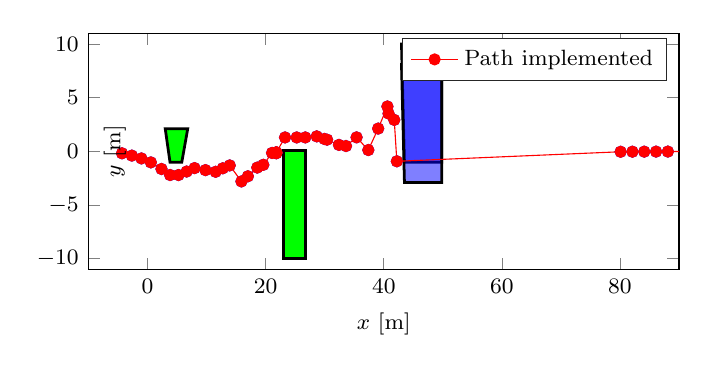
\begin{tikzpicture}

\begin{axis}[%
width=7.5cm,
height=3cm,
at={(3in,1in)},
scale only axis,
xmin=-10,
xmax=90,
%xlabel style={font=\color{white!15!black}},
xlabel={$x$ [\si{\meter}]},
font = \footnotesize,
ymin=-11,
ymax=11,
ylabel style={at={(0.08, 0.5)}},
ylabel={$y$ [\si{\meter}]},
axis background/.style={fill=white},
legend style={legend cell align=left, align=left, draw=white!15!black}
]

\addplot[area legend, line width=1.0pt, draw=black, fill=green, forget plot]
table[row sep=crcr] {%
x	y\\
3	2.1\\
6.8	2.1\\
5.8	-1\\
3.8	-1\\
}--cycle;



\addplot[area legend, line width=1.0pt, draw=black, fill=green, forget plot]
table[row sep=crcr] {%
x	y\\
23	0.1\\
26.8	0.1\\
26.8	-10\\
23	-10\\
}--cycle;


\addplot [color=blue, mark=o, mark options={solid, blue}, forget plot]
  table[row sep=crcr]{%
-4.32434674695592	-0.177804185117004\\
};


\addplot [color=blue, mark=o, mark options={solid, blue}, forget plot]
  table[row sep=crcr]{%
-2.65840571731513	-0.391529836390504\\
};


\addplot [color=blue, mark=o, mark options={solid, blue}, forget plot]
  table[row sep=crcr]{%
-1.03932716615722	-0.654331297723228\\
};


\addplot [color=blue, mark=o, mark options={solid, blue}, forget plot]
  table[row sep=crcr]{%
0.561087949854027	-1.02314889158218\\
};


\addplot [color=blue, mark=o, mark options={solid, blue}, forget plot]
  table[row sep=crcr]{%
2.36218692059051	-1.63816065798218\\
};


\addplot [color=blue, mark=o, mark options={solid, blue}, forget plot]
  table[row sep=crcr]{%
3.81552475353741	-2.2\\
};


\addplot [color=blue, mark=o, mark options={solid, blue}, forget plot]
  table[row sep=crcr]{%
5.23786219595455	-2.20246735051426\\
};


\addplot [color=blue, mark=o, mark options={solid, blue}, forget plot]
  table[row sep=crcr]{%
6.61852512418746	-1.87751017165566\\
};


\addplot [color=blue, mark=o, mark options={solid, blue}, forget plot]
  table[row sep=crcr]{%
7.95870480547107	-1.55679419196447\\
};


\addplot [color=blue, mark=o, mark options={solid, blue}, forget plot]
  table[row sep=crcr]{%
9.80748986836501	-1.74415191264204\\
};


\addplot [color=blue, mark=o, mark options={solid, blue}, forget plot]
  table[row sep=crcr]{%
11.5270608232353	-1.89882210273784\\
};


\addplot [color=blue, mark=o, mark options={solid, blue}, forget plot]
  table[row sep=crcr]{%
12.7367431613782	-1.57446562247343\\
};


\addplot [color=blue, mark=o, mark options={solid, blue}, forget plot]
  table[row sep=crcr]{%
13.9142651281089	-1.30551566298726\\
};


\addplot [color=blue, mark=o, mark options={solid, blue}, forget plot]
  table[row sep=crcr]{%
15.8961755980412	-2.79644354858628\\
};


\addplot [color=blue, mark=o, mark options={solid, blue}, forget plot]
  table[row sep=crcr]{%
16.9897015292746	-2.31875552011341\\
};


\addplot [color=blue, mark=o, mark options={solid, blue}, forget plot]
  table[row sep=crcr]{%
18.5787897905494	-1.50794234141928\\
};


\addplot [color=blue, mark=o, mark options={solid, blue}, forget plot]
  table[row sep=crcr]{%
19.6009962802512	-1.25035587789582\\
};

\addplot [color=blue, mark=o, mark options={solid, blue}, forget plot]
  table[row sep=crcr]{%
21.0815892207331	-0.142995979090026\\
};


\addplot [color=blue, mark=o, mark options={solid, blue}, forget plot]
  table[row sep=crcr]{%
21.7999999999998	-0.118569429387126\\
};


\addplot [color=blue, mark=o, mark options={solid, blue}, forget plot]
  table[row sep=crcr]{%
21.8	-0.17685244013917\\
};


\addplot [color=blue, mark=o, mark options={solid, blue}, forget plot]
  table[row sep=crcr]{%
21.7999999999999	-0.14664253531095\\
};


\addplot [color=blue, mark=o, mark options={solid, blue}, forget plot]
  table[row sep=crcr]{%
21.7999999999999	-0.121593081472356\\
};


\addplot [color=blue, mark=o, mark options={solid, blue}, forget plot]
  table[row sep=crcr]{%
21.7999999999999	-0.100822571231435\\
};


\addplot [color=blue, mark=o, mark options={solid, blue}, forget plot]
  table[row sep=crcr]{%
21.7999999999999	-0.0836000761444003\\
};


\addplot [color=blue, mark=o, mark options={solid, blue}, forget plot]
  table[row sep=crcr]{%
23.2803673707908	1.3\\
};


\addplot [color=blue, mark=o, mark options={solid, blue}, forget plot]
  table[row sep=crcr]{%
25.2614735760917	1.30038950533404\\
};


\addplot [color=blue, mark=o, mark options={solid, blue}, forget plot]
  table[row sep=crcr]{%
26.7112103924266	1.3\\
};


\addplot [color=blue, mark=o, mark options={solid, blue}, forget plot]
  table[row sep=crcr]{%
28.6479135939877	1.39955550406357\\
};


\addplot [color=blue, mark=o, mark options={solid, blue}, forget plot]
  table[row sep=crcr]{%
29.946062453838	1.15820116965655\\
};


\addplot [color=blue, mark=o, mark options={solid, blue}, forget plot]
  table[row sep=crcr]{%
30.4025591195175	1.0933950927041\\
};


\addplot [color=blue, mark=o, mark options={solid, blue}, forget plot]
  table[row sep=crcr]{%
32.4066267014977	0.606734100559028\\
};


\addplot [color=blue, mark=o, mark options={solid, blue}, forget plot]
  table[row sep=crcr]{%
33.6056515742852	0.500487026827704\\
};


\addplot [color=blue, mark=o, mark options={solid, blue}, forget plot]
  table[row sep=crcr]{%
35.3956390987588	1.30728808759823\\
};


\addplot [color=blue, mark=o, mark options={solid, blue}, forget plot]
  table[row sep=crcr]{%
37.383477371979	0.127795703300365\\
};


\addplot [color=blue, mark=o, mark options={solid, blue}, forget plot]
  table[row sep=crcr]{%
39.0539005824702	2.12662303252408\\
};


\addplot [color=blue, mark=o, mark options={solid, blue}, forget plot]
  table[row sep=crcr]{%
40.616481441141	4.18289140193312\\
};


\addplot [color=blue, mark=o, mark options={solid, blue}, forget plot]
  table[row sep=crcr]{%
40.8136768129359	3.52781758807466\\
};


\addplot [color=blue, mark=o, mark options={solid, blue}, forget plot]
  table[row sep=crcr]{%
41.7736571250654	2.93452882930331\\
};


\addplot [color=blue, mark=o, mark options={solid, blue}, forget plot]
  table[row sep=crcr]{%
42.2133819236134	-0.921660974219885\\
};


\addplot [color=blue, mark=o, mark options={solid, blue}, forget plot]
  table[row sep=crcr]{%
80.1064776734693	-0.0336733810702096\\
};


\addplot [color=blue, mark=o, mark options={solid, blue}, forget plot]
  table[row sep=crcr]{%
82.1064776734813	-0.0279212996367888\\
};


\addplot [color=blue, mark=o, mark options={solid, blue}, forget plot]
  table[row sep=crcr]{%
84.1064776734899	-0.0231517878107296\\
};


\addplot [color=blue, mark=o, mark options={solid, blue}, forget plot]
  table[row sep=crcr]{%
86.1064776734962	-0.0191970032128021\\
};


\addplot [color=blue, mark=o, mark options={solid, blue}, forget plot]
  table[row sep=crcr]{%
88.1064776735009	-0.0159177742714774\\
};


\addplot [color=blue, mark=o, mark options={solid, blue}, forget plot]
  table[row sep=crcr]{%
90.1064776735043	-0.0131987026802568\\
};


\addplot [color=blue, mark=o, mark options={solid, blue}, forget plot]
  table[row sep=crcr]{%
92.1064776735066	-0.0109441024524371\\
};


\addplot [color=blue, mark=o, mark options={solid, blue}, forget plot]
  table[row sep=crcr]{%
94.1064776735084	-0.00907463266587559\\
};


\addplot [color=blue, mark=o, mark options={solid, blue}, forget plot]
  table[row sep=crcr]{%
96.1064776735098	-0.00752450540174153\\
};


\addplot [color=blue, mark=o, mark options={solid, blue}, forget plot]
  table[row sep=crcr]{%
98.1064776735107	-0.00623917062271227\\
};
\addplot [color=blue, mark=o, mark options={solid, blue}, forget plot]
  table[row sep=crcr]{%
100.106477673511	-0.0051733965198969\\
};
\addplot [color=blue, mark=o, mark options={solid, blue}, forget plot]
  table[row sep=crcr]{%
102.106477673511	-0.00428967777458317\\
};
\addplot [color=blue, mark=o, mark options={solid, blue}, forget plot]
  table[row sep=crcr]{%
104.106477673512	-0.00355691572045193\\
};
\addplot [color=blue, mark=o, mark options={solid, blue}, forget plot]
  table[row sep=crcr]{%
106.106477673512	-0.00294932396026585\\
};
\addplot [color=blue, mark=o, mark options={solid, blue}, forget plot]
  table[row sep=crcr]{%
108.106477673512	-0.00244552092493577\\
};
\addplot [color=blue, mark=o, mark options={solid, blue}, forget plot]
  table[row sep=crcr]{%
110.106477673658	-0.00202777744162007\\
};
\addplot [color=blue, mark=o, mark options={solid, blue}, forget plot]
  table[row sep=crcr]{%
112.106477673763	-0.00168139283160677\\
};
\addplot [color=blue, mark=o, mark options={solid, blue}, forget plot]
  table[row sep=crcr]{%
114.10647767384	-0.00139417758386409\\
};
\addplot [color=blue, mark=o, mark options={solid, blue}, forget plot]
  table[row sep=crcr]{%
116.106477673898	-0.0011560243976318\\
};
\addplot [color=blue, mark=o, mark options={solid, blue}, forget plot]
  table[row sep=crcr]{%
118.106477673941	-0.000958552499611664\\
};
\addplot [color=black, mark=asterisk, mark options={solid, black}, forget plot]
  table[row sep=crcr]{%
118.106477673941	-0.000958552499611664\\
120.106477673975	-0.000794812718825946\\
122.106477674037	-0.000622429894945641\\
124.106477674101	-0.00047056871778238\\
126.106477674166	-0.000347533205760614\\
128.10647767423	-0.000252511773992365\\
130.106477674294	-0.00018132321744221\\
132.106477674357	-0.000129077180004821\\
134.10647767442	-9.12884042839382e-05\\
136.106477674482	-6.42464047630189e-05\\
138.106477674543	-4.50496638170494e-05\\
140.106477674601	-3.15069728758317e-05\\
142.106477674656	-2.2001665187446e-05\\
144.106477674706	-1.53604169852877e-05\\
146.10647767475	-1.07418509877084e-05\\
148.106477674787	-7.54791017959371e-06\\
150.106477674816	-5.35575762282959e-06\\
152.106477674838	-3.86605504911069e-06\\
154.106477674852	-2.86290137479817e-06\\
156.10647767486	-2.18036730506054e-06\\
158.106477674864	-1.66968838096488e-06\\
};
\addplot [color=blue, mark=o, mark options={solid, blue}, forget plot]
  table[row sep=crcr]{%
120.106477673975	-0.000794812718825946\\
};

\addplot[area legend, line width=1.0pt, draw=black, fill=blue, fill opacity=0.5, forget plot]
table[row sep=crcr] {%
x	y\\
43	10\\
49.8	10\\
49.8	-1\\
43.5	-1\\
}--cycle;

\addplot[area legend, line width=1.0pt, draw=black, fill=blue, fill opacity=0.5, forget plot]
table[row sep=crcr] {%
x	y\\
43	8.10000000000001\\
49.8	8.10000000000001\\
49.8	-2.9\\
43.5	-2.9\\
}--cycle;
\addplot [color=red, mark=*, mark options={solid, red}]
  table[row sep=crcr]{%
-4.32434674695592	-0.177804185117004\\
-2.65840571731513	-0.391529836390504\\
-1.03932716615722	-0.654331297723228\\
0.561087949854027	-1.02314889158218\\
2.36218692059051	-1.63816065798218\\
3.81552475353741	-2.2\\
5.23786219595455	-2.20246735051426\\
6.61852512418746	-1.87751017165566\\
7.95870480547107	-1.55679419196447\\
9.80748986836501	-1.74415191264204\\
11.5270608232353	-1.89882210273784\\
12.7367431613782	-1.57446562247343\\
13.9142651281089	-1.30551566298726\\
15.8961755980412	-2.79644354858628\\
16.9897015292746	-2.31875552011341\\
18.5787897905494	-1.50794234141928\\
19.6009962802512	-1.25035587789582\\
21.0815892207331	-0.142995979090026\\
21.7999999999998	-0.118569429387126\\
21.8	-0.17685244013917\\
21.7999999999999	-0.14664253531095\\
21.7999999999999	-0.121593081472356\\
21.7999999999999	-0.100822571231435\\
21.7999999999999	-0.0836000761444003\\
23.2803673707908	1.3\\
25.2614735760917	1.30038950533404\\
26.7112103924266	1.3\\
28.6479135939877	1.39955550406357\\
29.946062453838	1.15820116965655\\
30.4025591195175	1.0933950927041\\
32.4066267014977	0.606734100559028\\
33.6056515742852	0.500487026827704\\
35.3956390987588	1.30728808759823\\
37.383477371979	0.127795703300365\\
39.0539005824702	2.12662303252408\\
40.616481441141	4.18289140193312\\
40.8136768129359	3.52781758807466\\
41.7736571250654	2.93452882930331\\
42.2133819236134	-0.921660974219885\\
80.1064776734693	-0.0336733810702096\\
82.1064776734813	-0.0279212996367888\\
84.1064776734899	-0.0231517878107296\\
86.1064776734962	-0.0191970032128021\\
88.1064776735009	-0.0159177742714774\\
90.1064776735043	-0.0131987026802568\\
92.1064776735066	-0.0109441024524371\\
94.1064776735084	-0.00907463266587559\\
96.1064776735098	-0.00752450540174153\\
98.1064776735107	-0.00623917062271227\\
100.106477673511	-0.0051733965198969\\
102.106477673511	-0.00428967777458317\\
104.106477673512	-0.00355691572045193\\
106.106477673512	-0.00294932396026585\\
108.106477673512	-0.00244552092493577\\
110.106477673658	-0.00202777744162007\\
112.106477673763	-0.00168139283160677\\
114.10647767384	-0.00139417758386409\\
116.106477673898	-0.0011560243976318\\
118.106477673941	-0.000958552499611664\\
120.106477673975	-0.000794812718825946\\
};
\addlegendentry{Path implemented}
\end{axis}
\end{tikzpicture}%}\\
      \subfloat[$M$-analysis for scenario that resulting in dynamically unreasonable trajectory.\label{fig:badM}]{% This file was created by matlab2tikz.
%
%The latest updates can be retrieved from
%  http://www.mathworks.com/matlabcentral/fileexchange/22022-matlab2tikz-matlab2tikz
%where you can also make suggestions and rate matlab2tikz.
%
\definecolor{mycolor1}{rgb}{0.00000,0.44700,0.74100}%
%
\begin{tikzpicture}

\begin{axis}[%
width=7.5cm,
height=2.5cm,
at={(3in,1in)},
scale only axis,
bar shift auto,
xmin=-0.2,
xmax=61.2,
font = \footnotesize,
%xlabel style={font=\color{white!15!black}},
xlabel={$\text{k}^{\text{th}}\text{ action location}$},
ymin=0,
ymax=20,
ylabel style={at={(0.08, 0.5)}},
ylabel={$M$-stable},
axis background/.style={fill=white},
legend style={legend cell align=left, align=left, draw=white!15!black}
]
\addplot[ybar, bar width=3.5, fill=mycolor1, draw=black, area legend] table[row sep=crcr] {%
1	0\\
2	1\\
3	2\\
4	3\\
5	3\\
6	3\\
7	4\\
8	5\\
9	5\\
10	5\\
11	4\\
12	5\\
13	5\\
14	7\\
15	7\\
16	9\\
17	11\\
18	12\\
19	13\\
20	14\\
21	15\\
22	15\\
23	15\\
24	16\\
25	17\\
26	16\\
27	16\\
28	16\\
29	17\\
30	16\\
31	17\\
32	16\\
33	17\\
34	17\\
35	15\\
36	15\\
37	15\\
38	13\\
39	13\\
40	11\\
41	11\\
42	12\\
43	12\\
44	14\\
45	14\\
46	15\\
47	14\\
48	15\\
49	15\\
50	17\\
51	16\\
52	17\\
53	17\\
54	17\\
55	17\\
56	18\\
57	18\\
58	19\\
59	19\\
60	20\\
};
\addplot[forget plot, color=white!15!black] table[row sep=crcr] 
      
      \caption{Scenario resulting in dynamically unreasonable trajectory.}
      
\end{figure}



\subsection{Relationship between $M$ and $H$}

In industries, choosing a prediction horizon to be large enough is a common way to guarantee stability \cite{mayne2000constrained}. Therefore, we examined the relationship between the prediction horizon $H$ and the resulting $M$ for $M$-analysis. The scenario that has unknown moving obstacle is used here. Define the largest possible $M$ at each action location as $M_{max,k}$, where $M_{max,k} = k-1$ for $k\leq H+1$, and $M_{max,k} = H$ for $k>H+1$. In Fig.~\ref{fig:HM20}, systems with larger ($H>20$) prediction horizon reach $20$-settling (which is a guarantee that the location will not change much within 20 sampling steps before it is executed) faster than the system with $H=20$. Interestingly, all these systems reach $M=20$ in the range after $k=27$, which is the critical action location, but before $k=32$, whereas system with $H=20$ reaches $20$-settling not until after $k=45$. Figure~\ref{fig:HM} shows the smallest $M$ after $k$ reaches $H+1$ for each prediction horizon. It is clear that the smallest $M$ among all action location increase with $H$. Note that large $H$ makes the problem computationally heavy, which should be avoided if possible. We conclude that the horizon can be considered large enough if it can cover the last critical action location, in this case, when $H>27$.


 







\begin{figure}[t]
      \centering
      % This file was created by matlab2tikz.
%
%The latest updates can be retrieved from
%  http://www.mathworks.com/matlabcentral/fileexchange/22022-matlab2tikz-matlab2tikz
%where you can also make suggestions and rate matlab2tikz.
%
\definecolor{mycolor1}{rgb}{0.00000,0.44700,0.74100}%
\definecolor{mycolor2}{rgb}{0.85000,0.32500,0.09800}%
\definecolor{mycolor3}{rgb}{0.92900,0.69400,0.12500}%
\definecolor{mycolor4}{rgb}{0.49400,0.18400,0.55600}%
\definecolor{mycolor5}{rgb}{0.46600,0.67400,0.18800}%
%
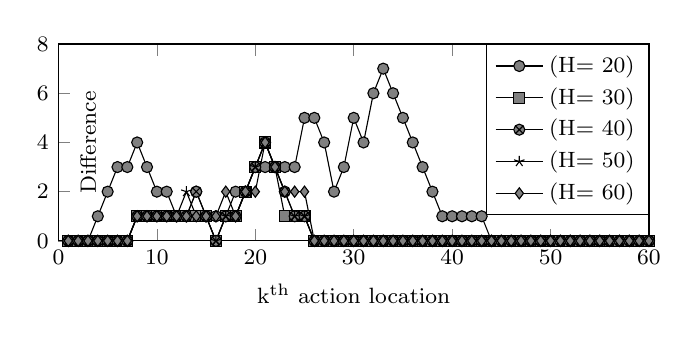
\begin{tikzpicture}

\begin{axis}[%
width=7.5cm,
height=2.5cm,
at={(3in,1in)},
scale only axis,
xmin=0,
xmax=60,
font = \footnotesize,
%xlabel style={font=\color{white!15!black}},
xlabel={$\text{k}^{\text{th}}\text{ action location}$},
ymin=0,
ymax=8,
ylabel style={at={(0.08, 0.5)}},
ylabel={Difference},
axis background/.style={fill=white},
%title style={font=\bfseries},
%title={$\text{Difference between simulated M and M}_{\text{Max,k}}\text{ at H=20}$},
%legend style={at={(1,1)},anchor=north east, legend cell align=left, align=left, draw=white!12!black}
legend style ={ at={(1,1)}, 
        anchor=north east, legend cell align=left, align=left},
    cycle list name=black white
]

\addplot 
  table[row sep=crcr]{%
1	0\\
2	0\\
3	0\\
4	1\\
5	2\\
6	3\\
7	3\\
8	4\\
9	3\\
10	2\\
11	2\\
12	1\\
13	1\\
14	2\\
15	1\\
16	1\\
17	1\\
18	2\\
19	2\\
20	3\\
21	3\\
22	3\\
23	3\\
24	3\\
25	5\\
26	5\\
27	4\\
28	2\\
29	3\\
30	5\\
31	4\\
32	6\\
33	7\\
34	6\\
35	5\\
36	4\\
37	3\\
38	2\\
39	1\\
40	1\\
41	1\\
42	1\\
43	1\\
44	0\\
45	0\\
46	0\\
47	0\\
48	0\\
49	0\\
50	0\\
51	0\\
52	0\\
53	0\\
54	0\\
55	0\\
56	0\\
57	0\\
58	0\\
59	0\\
60	0\\
};
\addlegendentry{(H= 20)}

\addplot
  table[row sep=crcr]{%
1	0\\
2	0\\
3	0\\
4	0\\
5	0\\
6	0\\
7	0\\
8	1\\
9	1\\
10	1\\
11	1\\
12	1\\
13	1\\
14	1\\
15	1\\
16	0\\
17	1\\
18	1\\
19	2\\
20	3\\
21	4\\
22	3\\
23	1\\
24	1\\
25	1\\
26	0\\
27	0\\
28	0\\
29	0\\
30	0\\
31	0\\
32	0\\
33	0\\
34	0\\
35	0\\
36	0\\
37	0\\
38	0\\
39	0\\
40	0\\
41	0\\
42	0\\
43	0\\
44	0\\
45	0\\
46	0\\
47	0\\
48	0\\
49	0\\
50	0\\
51	0\\
52	0\\
53	0\\
54	0\\
55	0\\
56	0\\
57	0\\
58	0\\
59	0\\
60	0\\
};
\addlegendentry{(H= 30)}

\addplot 
  table[row sep=crcr]{%
1	0\\
2	0\\
3	0\\
4	0\\
5	0\\
6	0\\
7	0\\
8	1\\
9	1\\
10	1\\
11	1\\
12	1\\
13	1\\
14	2\\
15	1\\
16	0\\
17	1\\
18	1\\
19	2\\
20	3\\
21	4\\
22	3\\
23	2\\
24	1\\
25	1\\
26	0\\
27	0\\
28	0\\
29	0\\
30	0\\
31	0\\
32	0\\
33	0\\
34	0\\
35	0\\
36	0\\
37	0\\
38	0\\
39	0\\
40	0\\
41	0\\
42	0\\
43	0\\
44	0\\
45	0\\
46	0\\
47	0\\
48	0\\
49	0\\
50	0\\
51	0\\
52	0\\
53	0\\
54	0\\
55	0\\
56	0\\
57	0\\
58	0\\
59	0\\
60	0\\
};
\addlegendentry{(H= 40)}

\addplot 
  table[row sep=crcr]{%
1	0\\
2	0\\
3	0\\
4	0\\
5	0\\
6	0\\
7	0\\
8	1\\
9	1\\
10	1\\
11	1\\
12	1\\
13	2\\
14	1\\
15	1\\
16	0\\
17	1\\
18	1\\
19	2\\
20	3\\
21	4\\
22	3\\
23	2\\
24	1\\
25	1\\
26	0\\
27	0\\
28	0\\
29	0\\
30	0\\
31	0\\
32	0\\
33	0\\
34	0\\
35	0\\
36	0\\
37	0\\
38	0\\
39	0\\
40	0\\
41	0\\
42	0\\
43	0\\
44	0\\
45	0\\
46	0\\
47	0\\
48	0\\
49	0\\
50	0\\
51	0\\
52	0\\
53	0\\
54	0\\
55	0\\
56	0\\
57	0\\
58	0\\
59	0\\
60	0\\
};
\addlegendentry{(H= 50)}

\addplot 
  table[row sep=crcr]{%
1	0\\
2	0\\
3	0\\
4	0\\
5	0\\
6	0\\
7	0\\
8	1\\
9	1\\
10	1\\
11	1\\
12	1\\
13	1\\
14	1\\
15	1\\
16	1\\
17	2\\
18	1\\
19	2\\
20	2\\
21	4\\
22	3\\
23	2\\
24	2\\
25	2\\
26	0\\
27	0\\
28	0\\
29	0\\
30	0\\
31	0\\
32	0\\
33	0\\
34	0\\
35	0\\
36	0\\
37	0\\
38	0\\
39	0\\
40	0\\
41	0\\
42	0\\
43	0\\
44	0\\
45	0\\
46	0\\
47	0\\
48	0\\
49	0\\
50	0\\
51	0\\
52	0\\
53	0\\
54	0\\
55	0\\
56	0\\
57	0\\
58	0\\
59	0\\
60	0\\
};
\addlegendentry{(H= 60)}

\end{axis}
\end{tikzpicture}% 
      \caption{Difference between simulated $M$ and $M_{max,k}$ for $H=20$ (with speed change). }
      \label{fig:HM20}
\end{figure}

\begin{figure}[t]
      \centering
      % This file was created by matlab2tikz.
%
%The latest updates can be retrieved from
%  http://www.mathworks.com/matlabcentral/fileexchange/22022-matlab2tikz-matlab2tikz
%where you can also make suggestions and rate matlab2tikz.
%
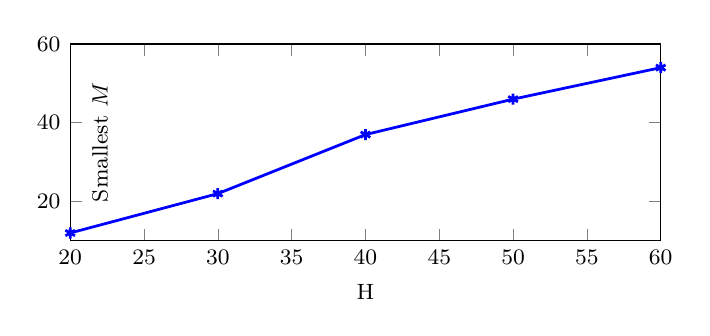
\begin{tikzpicture}

\begin{axis}[%
width=7.5cm,
height=2.5cm,
at={(3in,1in)},
scale only axis,
xmin=20,
xmax=60,
%xlabel style={font=\color{white!15!black}},
xlabel={H},
ymin=10,
ymax=60,
font = \footnotesize,
ylabel style={at={(0.08, 0.5)}},
ylabel={Smallest $M$},
axis background/.style={fill=white},
%title style={font=\bfseries},
%title={Smallest M for each prediction horizon},
legend style={legend cell align=left, align=left, draw=white!15!black}
]
\addplot [color=blue, line width=1.0pt, mark=asterisk, mark options={solid, blue}]
  table[row sep=crcr]{%
20	12\\
30	22\\
40	37\\
50	46\\
60	54\\
};


\end{axis}
\end{tikzpicture}% 
      \caption{Smallest $M$ for each prediction horizon. }
      \label{fig:HM}
\end{figure}


\begin{figure*}
 \centering
  \begin{tabular}{@{}ccc@{}}
  
   \begin{minipage}{.3\textwidth}
    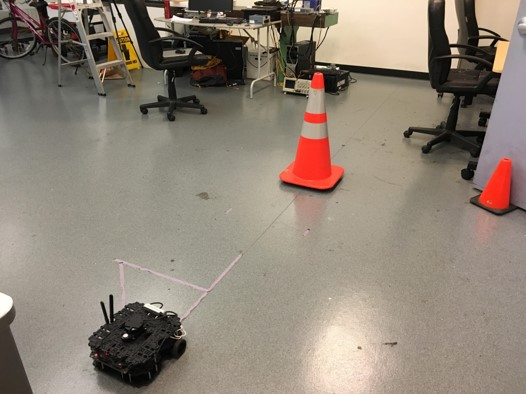
\includegraphics[width=\textwidth]{plot/tu1.jpg}
   \captionof*{figure}{At time step t=2}
   \end{minipage} &
    \begin{minipage}{.3\textwidth}
    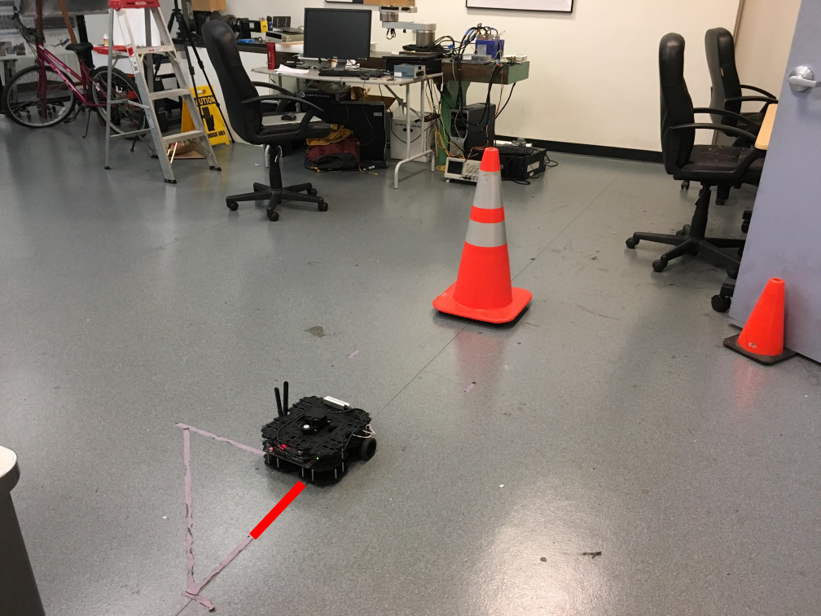
\includegraphics[width=\textwidth]{plot/tu2.png}
   \captionof*{figure}{At time step t=32}
   \end{minipage} &
      \begin{minipage}{.3\textwidth}
    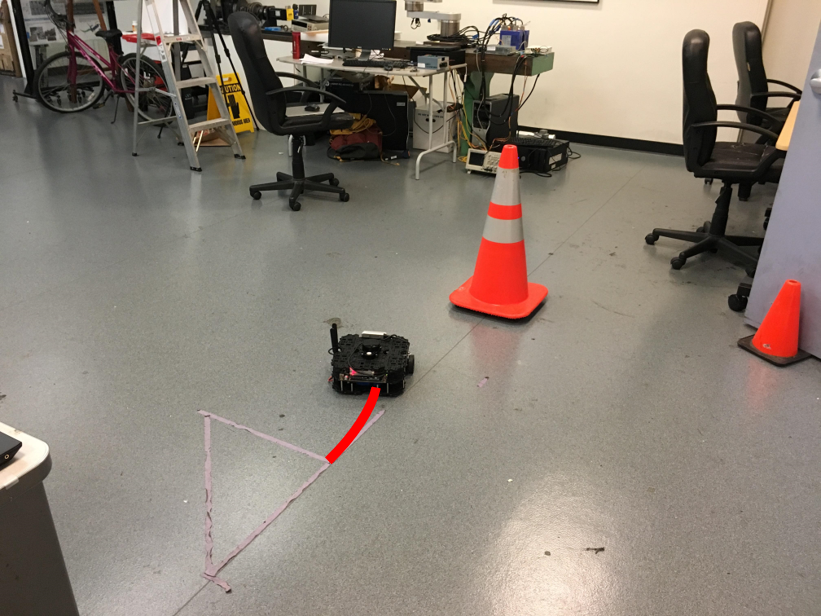
\includegraphics[width=\textwidth]{plot/tu3.png}
   \captionof*{figure}{At time step t=41}
   \end{minipage}\\
      \begin{minipage}{.3\textwidth}
    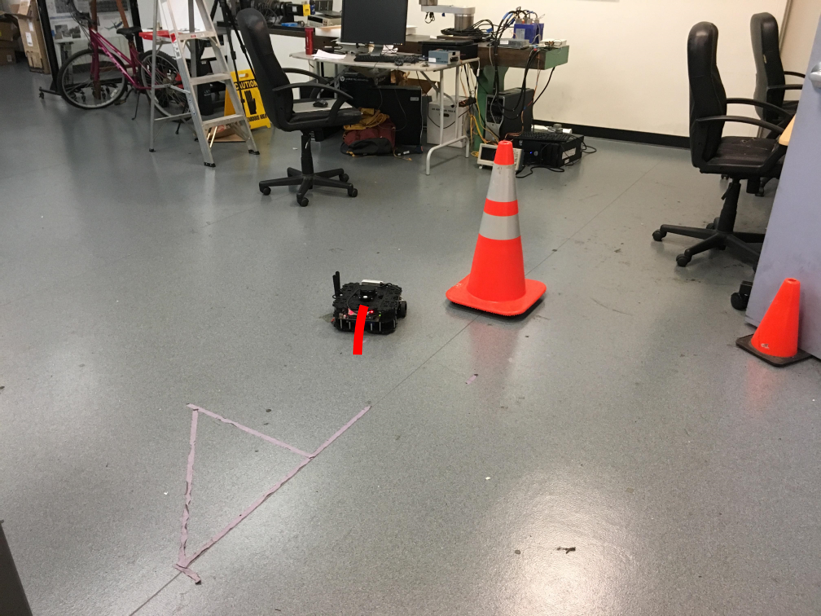
\includegraphics[width=\textwidth]{plot/tu4.png}
   \captionof*{figure}{At time step t=57}
   \end{minipage} &
    \begin{minipage}{.3\textwidth}
    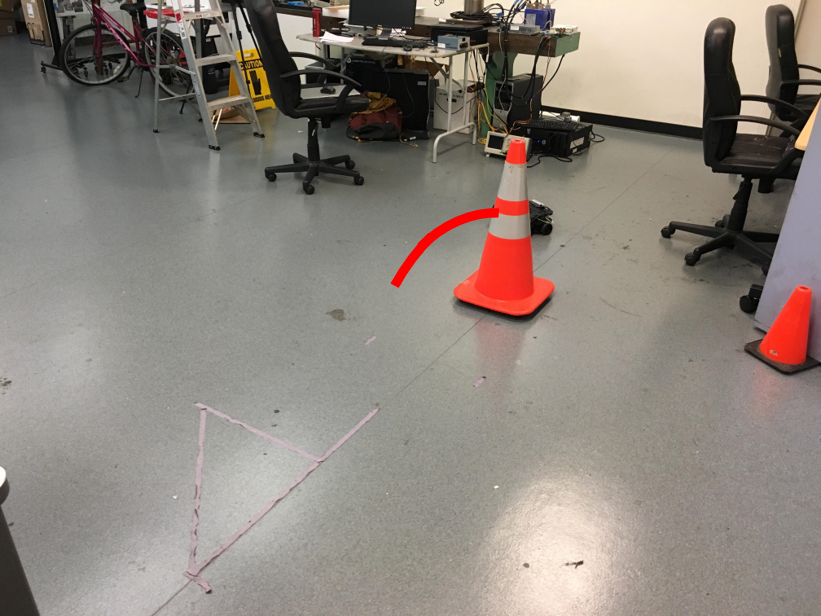
\includegraphics[width=\textwidth]{plot/tu5.png}
    \captionof*{figure}{At time step t=80}
   \end{minipage} &
      \begin{minipage}{.3\textwidth}
    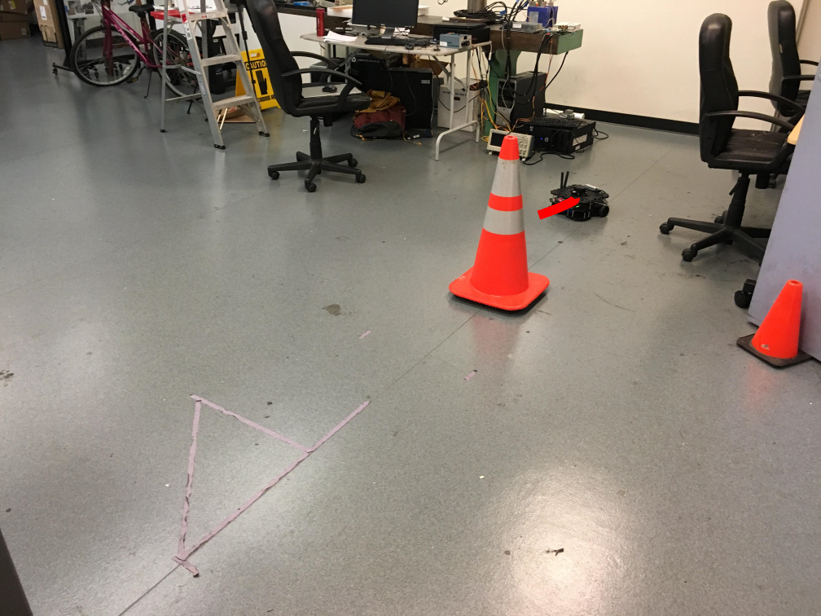
\includegraphics[width=\textwidth]{plot/tu6.png}
    \captionof*{figure}{At time step t=91}
   \end{minipage}\\
  \end{tabular}
  \caption{Experiment result of robot avoiding an obstacle.}
  \label{fig:ex}
\end{figure*} 


\section{EXPERIMENT RESULT}

\subsection{Experiment set up}
To verify whether the planned trajectory is dynamically reasonable for a mobile robot to execute, the MPC-CFS (with $H=20$) controller is tested on TurtleBot3, which is  developed by ROBOTIS. TurtleBot3 is a ROS standard platform robot. The MPC-CFS controller is running in MATLAB on a separate laptop with an 2.8GHz Intel Core i7-7700HQ.

Since the dynamics is not included in the MPC problem, we need an additional tracking controller to calculate the suitable command for the robot to execute the planned trajectory. Here we used an iterative LQR (ILQR) controller \cite{tassa2012synthesis}. The cost function is designed to minimize the tracking error and also the robot's acceleration. The final control input at the first time step is chosen to be the the control command for the robot.

\subsection{Experiment result}
Similar to the simulation, the goal for the robot is to move along a line, $y=0$, in the positive $x$-axis direction, while avoiding obstacles and maintaining constant speed which also points along the positive $x$-axis.

The experiment result is shown in Fig.~\ref{fig:ex} and Fig.~\ref{fig:trajectory}, where we can see that the robot can successfully avoid the obstacle and merge back to the original route. Control command is shown in Fig.~\ref{fig:command}.

The proposed $M$-analysis can also be applied in this scenario. If we use the original planning problem ((1)$\sim$(3)), the infeasible starting state at each time step will cause the robot to move in a violent manner. However, after introducing slack variables, the planning results in smoother trajectory. From Fig.~\ref{fig:msettling} we can see that after the first several steps, the whole system maintains at least $13$-settling. After passing by the obstacle ($k>80$), $M$ goes to and maintains at $20$, which indicates that the robot has settled back to track $y=0$. 


\begin{figure}[t]
      \centering
      % This file was created by matlab2tikz.
%
%The latest updates can be retrieved from
%  http://www.mathworks.com/matlabcentral/fileexchange/22022-matlab2tikz-matlab2tikz
%where you can also make suggestions and rate matlab2tikz.
%
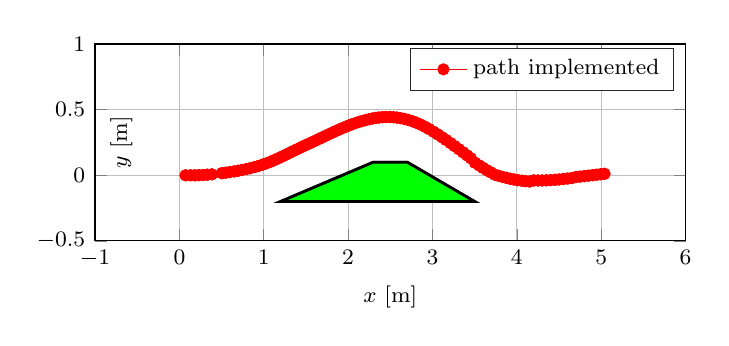
\begin{tikzpicture}

\begin{axis}[%
width=7.5cm,
height=2.5cm,
at={(3in,1in)},
scale only axis,
xmin=-1,
xmax=6,
%xlabel style={font=\color{white!15!black}},
xlabel={$x$ [\si{\meter}]},
ymin=-0.5,
ymax=1,
font = \footnotesize,
ylabel style={at={(0.08, 0.5)}},
ylabel={$y$ [\si{\meter}]},
axis background/.style={fill=white},
%title style={font=\bfseries},
%title={Implemented trajectory},
xmajorgrids,
ymajorgrids,
legend style={legend cell align=left, align=left, draw=white!15!black}
]
\addplot [color=red, mark=*, mark options={solid, red}, forget plot]
  table[row sep=crcr]{%
0.0737134865191896	-0.000197470377270626\\
0.133154712607953	-0.000190842012033869\\
0.183399988264539	-0.000105818851838134\\
0.229340919771424	0.000703715276970473\\
0.281357126463957	0.00209840982752709\\
0.33222073506804	0.00420792229507388\\
0.384144590832578	0.00712725339853666\\
0.504126487054251	0.0159576984655284\\
0.549746753128694	0.0196671918201685\\
0.595086521121512	0.0238618517992169\\
0.648855485861408	0.0293476807919532\\
0.696067739913624	0.0342880969611617\\
0.742502649981113	0.0401682130112322\\
0.792763190605092	0.0467850834767557\\
0.840037092371348	0.0541523298975717\\
0.889156630781511	0.0621847059506082\\
0.934730802432578	0.0703600502804331\\
0.983584857613806	0.0803789423861068\\
1.03116190744374	0.0910254391747426\\
1.08282630073162	0.103518107266157\\
1.1279583394536	0.116151318175265\\
1.17560813314594	0.129868165358204\\
1.2170637901593	0.142633538725222\\
1.26249012502438	0.156722641779588\\
1.30757965163828	0.170904717160431\\
1.35073908375145	0.184593718783195\\
1.39557603709353	0.198498058417477\\
1.43945719728905	0.212121169213491\\
1.48065173534724	0.224487501928063\\
1.52293853048789	0.237320208208805\\
1.56848596413989	0.250491853435777\\
1.6100431497922	0.263069502960802\\
1.65514291806029	0.276935015931691\\
1.69355593798644	0.288552469190672\\
1.73757302774198	0.3021339694372\\
1.77286230088404	0.312704981815203\\
1.81347011649436	0.32488998702302\\
1.85408929683634	0.336859325446405\\
1.89051278135041	0.347417975172901\\
1.92917632486848	0.358477750854422\\
1.97231709358059	0.369621390547016\\
2.01006683767719	0.379768377292742\\
2.0494524580619	0.389462867175559\\
2.09038366056946	0.398570020559115\\
2.13011932457405	0.406815134666448\\
2.16841421004693	0.413788777962393\\
2.20781742311312	0.420600475661087\\
2.24863421237336	0.427223191927311\\
2.28876450557806	0.432569806360068\\
2.32744755612542	0.436959513557654\\
2.36403676274451	0.440086635418948\\
2.40647759971467	0.44263420237485\\
2.44696176066306	0.443828183076265\\
2.49323886413279	0.443918557656909\\
2.5369133611192	0.442324938699292\\
2.57855417759534	0.439492134508098\\
2.61958380437843	0.435355546163741\\
2.66681179329944	0.429318273852274\\
2.7143273107976	0.421384889020811\\
2.76177394542984	0.41173110176049\\
2.80915527196148	0.4000873085876\\
2.85663451286562	0.386891982172109\\
2.91127843274611	0.369679934263898\\
2.95987083395438	0.351972243135213\\
3.01294311284782	0.33146374061209\\
3.06420750952867	0.310636293247374\\
3.11523813770994	0.288630080864784\\
3.16143540336703	0.268613700769736\\
3.21511457162527	0.244810762011187\\
3.26207443008977	0.222234611873333\\
3.31313091009319	0.19857568626525\\
3.36258707620506	0.174858033912087\\
3.41225789797535	0.150806593989002\\
3.4554336480909	0.129184070512743\\
3.50420694878975	0.0955608459189933\\
3.55549996125723	0.0743169646634031\\
3.59719756075071	0.0567965760829771\\
3.6463489708608	0.0378389264190291\\
3.69000325583708	0.0226404953727926\\
3.73827923387654	0.0046067794108847\\
3.78615340854023	-0.00466775533175003\\
3.83242023531502	-0.0129131310776917\\
3.87725643908207	-0.0202578545995929\\
3.92291512981734	-0.0267947133816753\\
3.9660543510313	-0.032357285777696\\
4.01126356791095	-0.0374240869191187\\
4.05893620866977	-0.0418244607258465\\
4.10512332496732	-0.0451817989432508\\
4.14977267331691	-0.0474673011008662\\
4.20101313020268	-0.0393956771036758\\
4.25014018344114	-0.0399398542361714\\
4.30071460445504	-0.0396883430296901\\
4.34977905872027	-0.0386532308422776\\
4.40223753996815	-0.0368946875670761\\
4.45421841459864	-0.0345611645849018\\
4.49952462894151	-0.031933269177163\\
4.55044673183439	-0.0286987583490714\\
4.60277975841777	-0.0250267644770024\\
4.65319674081469	-0.0210241623072232\\
4.70000277908854	-0.0136839941832646\\
4.7490913385793	-0.0103191945787484\\
4.79856331187578	-0.0067296018955853\\
4.84936461613002	-0.00302958242516053\\
4.89791537889276	0.000647819635826603\\
4.94713208453985	0.00429326759545361\\
4.99246008216514	0.00778236641081839\\
5.03864850084823	0.010995876325498\\
};



\addplot[area legend, line width=1.0pt, draw=black, fill=green, forget plot]
table[row sep=crcr] {%
x	y\\
2.3	0.1\\
2.7	0.1\\
3.5	-0.2\\
1.2	-0.2\\
}--cycle;


\addplot [color=red, mark=*, mark options={solid, red}]
  table[row sep=crcr]{%
0.0737134865191896	-0.000197470377270626\\
0.133154712607953	-0.000190842012033869\\
0.183399988264539	-0.000105818851838134\\
0.229340919771424	0.000703715276970473\\
0.281357126463957	0.00209840982752709\\
0.33222073506804	0.00420792229507388\\
0.384144590832578	0.00712725339853666\\
0.504126487054251	0.0159576984655284\\
0.549746753128694	0.0196671918201685\\
0.595086521121512	0.0238618517992169\\
0.648855485861408	0.0293476807919532\\
0.696067739913624	0.0342880969611617\\
0.742502649981113	0.0401682130112322\\
0.792763190605092	0.0467850834767557\\
0.840037092371348	0.0541523298975717\\
0.889156630781511	0.0621847059506082\\
0.934730802432578	0.0703600502804331\\
0.983584857613806	0.0803789423861068\\
1.03116190744374	0.0910254391747426\\
1.08282630073162	0.103518107266157\\
1.1279583394536	0.116151318175265\\
1.17560813314594	0.129868165358204\\
1.2170637901593	0.142633538725222\\
1.26249012502438	0.156722641779588\\
1.30757965163828	0.170904717160431\\
1.35073908375145	0.184593718783195\\
1.39557603709353	0.198498058417477\\
1.43945719728905	0.212121169213491\\
1.48065173534724	0.224487501928063\\
1.52293853048789	0.237320208208805\\
1.56848596413989	0.250491853435777\\
1.6100431497922	0.263069502960802\\
1.65514291806029	0.276935015931691\\
1.69355593798644	0.288552469190672\\
1.73757302774198	0.3021339694372\\
1.77286230088404	0.312704981815203\\
1.81347011649436	0.32488998702302\\
1.85408929683634	0.336859325446405\\
1.89051278135041	0.347417975172901\\
1.92917632486848	0.358477750854422\\
1.97231709358059	0.369621390547016\\
2.01006683767719	0.379768377292742\\
2.0494524580619	0.389462867175559\\
2.09038366056946	0.398570020559115\\
2.13011932457405	0.406815134666448\\
2.16841421004693	0.413788777962393\\
2.20781742311312	0.420600475661087\\
2.24863421237336	0.427223191927311\\
2.28876450557806	0.432569806360068\\
2.32744755612542	0.436959513557654\\
2.36403676274451	0.440086635418948\\
2.40647759971467	0.44263420237485\\
2.44696176066306	0.443828183076265\\
2.49323886413279	0.443918557656909\\
2.5369133611192	0.442324938699292\\
2.57855417759534	0.439492134508098\\
2.61958380437843	0.435355546163741\\
2.66681179329944	0.429318273852274\\
2.7143273107976	0.421384889020811\\
2.76177394542984	0.41173110176049\\
2.80915527196148	0.4000873085876\\
2.85663451286562	0.386891982172109\\
2.91127843274611	0.369679934263898\\
2.95987083395438	0.351972243135213\\
3.01294311284782	0.33146374061209\\
3.06420750952867	0.310636293247374\\
3.11523813770994	0.288630080864784\\
3.16143540336703	0.268613700769736\\
3.21511457162527	0.244810762011187\\
3.26207443008977	0.222234611873333\\
3.31313091009319	0.19857568626525\\
3.36258707620506	0.174858033912087\\
3.41225789797535	0.150806593989002\\
3.4554336480909	0.129184070512743\\
3.50420694878975	0.0955608459189933\\
3.55549996125723	0.0743169646634031\\
3.59719756075071	0.0567965760829771\\
3.6463489708608	0.0378389264190291\\
3.69000325583708	0.0226404953727926\\
3.73827923387654	0.0046067794108847\\
3.78615340854023	-0.00466775533175003\\
3.83242023531502	-0.0129131310776917\\
3.87725643908207	-0.0202578545995929\\
3.92291512981734	-0.0267947133816753\\
3.9660543510313	-0.032357285777696\\
4.01126356791095	-0.0374240869191187\\
4.05893620866977	-0.0418244607258465\\
4.10512332496732	-0.0451817989432508\\
4.14977267331691	-0.0474673011008662\\
4.20101313020268	-0.0393956771036758\\
4.25014018344114	-0.0399398542361714\\
4.30071460445504	-0.0396883430296901\\
4.34977905872027	-0.0386532308422776\\
4.40223753996815	-0.0368946875670761\\
4.45421841459864	-0.0345611645849018\\
4.49952462894151	-0.031933269177163\\
4.55044673183439	-0.0286987583490714\\
4.60277975841777	-0.0250267644770024\\
4.65319674081469	-0.0210241623072232\\
4.70000277908854	-0.0136839941832646\\
4.7490913385793	-0.0103191945787484\\
4.79856331187578	-0.0067296018955853\\
4.84936461613002	-0.00302958242516053\\
4.89791537889276	0.000647819635826603\\
4.94713208453985	0.00429326759545361\\
4.99246008216514	0.00778236641081839\\
5.03864850084823	0.010995876325498\\
};

\legend{path implemented};

\addplot[area legend, line width=1.0pt, draw=black, fill=green]
table[row sep=crcr] {%
x	y\\
2.3	0.1\\
2.7	0.1\\
3.5	-0.2\\
1.2	-0.2\\
}--cycle;


\end{axis}
\end{tikzpicture}% 
      \caption{ Implemented trajectory in the experiment. }
      \label{fig:trajectory}
\end{figure}

\begin{figure}[t]
      \centering
      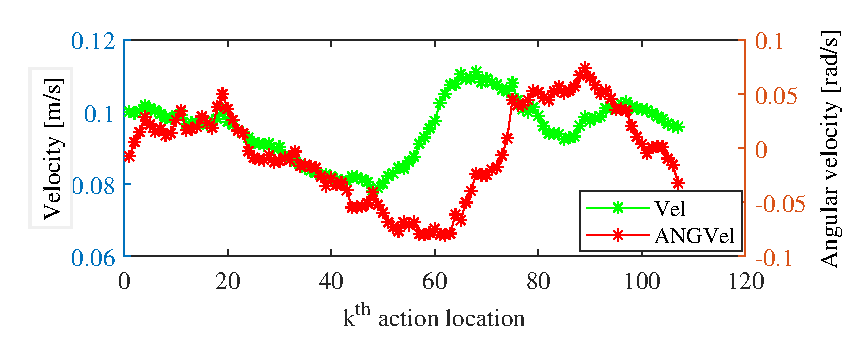
\includegraphics[width=9cm]{plot/video_nice.eps}
      
      \caption{Control command in the experiment. }
      \label{fig:command}
\end{figure}

\begin{figure}[t]
      \centering
      % This file was created by matlab2tikz.
%
%The latest updates can be retrieved from
%  http://www.mathworks.com/matlabcentral/fileexchange/22022-matlab2tikz-matlab2tikz
%where you can also make suggestions and rate matlab2tikz.
%
\definecolor{mycolor1}{rgb}{0.00000,0.44700,0.74100}%
%
\begin{tikzpicture}

\begin{axis}[%
width=7.5cm,
height=2.5cm,
at={(3in,1in)},
scale only axis,
bar shift auto,
xmin=-0.2,
xmax=108.2,
%xlabel style={font=\color{white!15!black}},
xlabel={$\text{k}^{\text{th}}\text{ action location}$},
ymin=0,
ymax=20,
font = \footnotesize,
ylabel style={at={(0.08, 0.5)}},
ylabel={$M$-stable},
axis background/.style={fill=white},
%title style={font=\bfseries},
%title={M-analysis for each action location},
legend style={legend cell align=left, align=left, draw=white!15!black}
]
\addplot[ybar, bar width=1.5, fill=mycolor1, draw=black, area legend] table[row sep=crcr] {%
1	0\\
2	1\\
3	2\\
4	3\\
5	4\\
6	5\\
7	6\\
8	6\\
9	7\\
10	8\\
11	9\\
12	10\\
13	11\\
14	11\\
15	12\\
16	13\\
17	14\\
18	15\\
19	16\\
20	16\\
21	16\\
22	17\\
23	17\\
24	17\\
25	16\\
26	18\\
27	17\\
28	17\\
29	17\\
30	17\\
31	17\\
32	17\\
33	17\\
34	17\\
35	17\\
36	17\\
37	16\\
38	16\\
39	15\\
40	15\\
41	14\\
42	14\\
43	15\\
44	15\\
45	15\\
46	14\\
47	15\\
48	14\\
49	14\\
50	15\\
51	15\\
52	15\\
53	15\\
54	15\\
55	17\\
56	16\\
57	17\\
58	17\\
59	17\\
60	17\\
61	18\\
62	18\\
63	17\\
64	17\\
65	17\\
66	18\\
67	17\\
68	18\\
69	17\\
70	18\\
71	19\\
72	20\\
73	20\\
74	20\\
75	20\\
76	19\\
77	19\\
78	18\\
79	16\\
80	18\\
81	18\\
82	18\\
83	18\\
84	19\\
85	19\\
86	19\\
87	19\\
88	19\\
89	19\\
90	19\\
91	19\\
92	19\\
93	19\\
94	19\\
95	19\\
96	19\\
97	19\\
98	20\\
99	20\\
100	20\\
101	20\\
102	20\\
103	20\\
104	20\\
105	20\\
106	20\\
107	20\\
};
\addplot[forget plot, color=white!15!black] table[row sep=crcr] {%
-0.2	0\\
108.2	0\\
};



\end{axis}
\end{tikzpicture}% 
      \caption{$M$-analysis for the experiment. }
      \label{fig:msettling}
\end{figure}





\section{Conclusion}

This paper proposed a new method of analyzing stability properties for non-convex MPC. The proposed method, $M$-analysis, considered the difference of each action location planned at consecutive time steps. We said the action location $k$ is $M$-settling if there is smaller and smaller change between consecutive time steps after time step $k-M$ which indicates local conversions of the planned trajectory. Simulation results showed that a robot that implemented the MPC-CFS algorithm was capable of dealing with dynamic environment as long as the changes in the environment were predictable. The stability analysis using $M$-analysis was performed to show that MPC-CFS had decent stability properties. Finally, experiment on Turtlebot3 showed that the proposed MPC-CFS controller performed well. In the future, we will include the robot dynamics in to the optimization problem formulation and complete the theoretical proof for $M$-analysis. 



\bibliography{root(ACC)}
\bibliographystyle{IEEEtran}


\end{document}







